% % ****** Start of file apssamp.tex ******
% %
% %   This file is part of the APS files in the REVTeX 4.1 distribution.
% %   Version 4.1r of REVTeX, August 2010
% %
% %   Copyright (c) 2009, 2010 The American Physical Society.
% %
% %   See the REVTeX 4 README file for restrictions and more information.
% %
% % TeX'ing this file requires that you have AMS-LaTeX 2.0 installed
% % as well as the rest of the prerequisites for REVTeX 4.1
% %
% % See the REVTeX 4 README file
% % It also requires running BibTeX. The commands are as follows:
% %
% %  1)  latex apssamp.tex
% %  2)  bibtex apssamp
% %  3)  latex apssamp.tex
% %  4)  latex apssamp.tex
% %
% \documentclass[%
%  reprint,
% superscriptaddress,
% onecolumn,
% linenumbers,
% notitlepage,
% %groupedaddress,
% %unsortedaddress,
% %runinaddress,
% %frontmatterverbose, 
% %preprint,
% %showpacs,preprintnumbers,
% %nofootinbib,
% %nobibnotes,
% %bibnotes,
%  amsmath,amssymb,
%  aps,
% prc,
% %prb,
% %rmp,
% %prstab,
% %prstper,
% %floatfix,
% ]{revtex4-1}
%%%%%%%%%%%%%%%%%%%%%%%%%%%%%%%%%%%%%%%%%%%%%%
%%%%%%%%%%%%%%%%%%%%%%%%%%%%%%%%%%%%%%%%%%%%%%
%%                                          %%
%% Important note on usage                  %%
%% -----------------------                  %%
%% This file must be compiled with PDFLaTeX %%
%% Using standard LaTeX will not work!      %%
%%                                          %%
%%%%%%%%%%%%%%%%%%%%%%%%%%%%%%%%%%%%%%%%%%%%%%
%%%%%%%%%%%%%%%%%%%%%%%%%%%%%%%%%%%%%%%%%%%%%%

%% The '3p' and 'times' class options of elsarticle are used for Elsevier CRC
% \documentclass[5p]{elsarticle}
% Good for final formatting  - two column
% 
% \documentclass[3p,times]{elsarticle}
% Final formatting
\documentclass[3p]{elsarticle}
% Good for proofing - single column
% 

\usepackage[american]{babel}
\usepackage{amsmath}
\usepackage[version=3]{mhchem} 
% \usepackage{fixltx2e}
% \usepackage{refcount}
% \usepackage{siunitx}
% \usepackage{lastpage}
% \usepackage{textcomp}
\usepackage{mathtools}

\usepackage{xfrac}
\usepackage{lmodern}
\usepackage[hidelinks]{hyperref}
% \usepackage{cool}
% \usepackage{cancel}
\usepackage{microtype}
\usepackage{listings}
\usepackage{mcode}
\usepackage [autostyle, english = american]{csquotes}
% \usepackage{longtable}
\usepackage{subcaption}
\usepackage{booktabs,siunitx}
\usepackage{gensymb}
\usepackage[normalem]{ulem}

% \usepackage{mathtools, cuted}


% \usepackage[usenames,dvipsnames,svgnames,table]{xcolor}
\usepackage{color}

\usepackage[colorinlistoftodos]{todonotes}

\usepackage[section]{placeins}
\usepackage{multirow}

\usepackage{lineno}

\usepackage{graphicx}% Include figure files
\usepackage{dcolumn}% Align table columns on decimal point
\usepackage{bm}% bold math



\lstset{basicstyle=\small\ttfamily,columns=fullflexible}

% \usepackage{verbatim}



% \usepackage{gensymb}
% \usepackage{enumerate}
% \usepackage{float}
% \usepackage{bm}
% \usepackage{csquotes}
% \usepackage{mathtools}
% \usepackage[sort&compress]{natbib}
% \usepackage{biblatex}

%% The `ecrc' package must be called to make the CRC functionality available
\usepackage{ecrc}

%% The ecrc package defines commands needed for running heads and logos.
%% For running heads, you can set the journal name, the volume, the starting page and the authors

%% set the volume if you know. Otherwise `00'
\volume{00}

%% set the starting page if not 1
\firstpage{1}

%% Give the name of the journal
\journalname{Nuclear Instruments and Methods in Physics Research B}

%% Give the author list to appear in the running head
%% Example \runauth{C.V. Radhakrishnan et al.}
\runauth{A.S. Voyles et al.}

%% The choice of journal logo is determined by the \jid and \jnltitlelogo commands.
%% A user-supplied logo with the name <\jid>logo.pdf will be inserted if present.
%% e.g. if \jid{yspmi} the system will look for a file yspmilogo.pdf
%% Otherwise the content of \jnltitlelogo will be set between horizontal lines as a default logo

%% Give the abbreviation of the Journal.
\jid{nimb}
% \jid{yspmi}

%% Give a short journal name for the dummy logo (if needed)
\jnltitlelogo{Nucl Instrum Meth B}

%% Hereafter the template follows `elsarticle'.
%% For more details see the existing template files elsarticle-template-harv.tex and elsarticle-template-num.tex.

%% Elsevier CRC generally uses a numbered reference style
%% For this, the conventions of elsarticle-template-num.tex should be followed (included below)
%% If using BibTeX, use the style file elsarticle-num.bst

%% End of ecrc-specific commands
%%%%%%%%%%%%%%%%%%%%%%%%%%%%%%%%%%%%%%%%%%%%%%%%%%%%%%%%%%%%%%%%%%%%%%%%%%

%% The amssymb package provides various useful mathematical symbols
\usepackage{amssymb}
%% The amsthm package provides extended theorem environments
\usepackage{amsthm}

%% The lineno packages adds line numbers. Start line numbering with
%% \begin{linenumbers}, end it with \end{linenumbers}. Or switch it on
%% for the whole article with \linenumbers after \end{frontmatter}.
%% \usepackage{lineno}

%% natbib.sty is loaded by default. However, natbib options can be
%% provided with \biboptions{...} command. Following options are
%% valid:

%%   round  -  round parentheses are used (default)
%%   square -  square brackets are used   [option]
%%   curly  -  curly braces are used      {option}
%%   angle  -  angle brackets are used    <option>
%%   semicolon  -  multiple citations separated by semi-colon
%%   colon  - same as semicolon, an earlier confusion
%%   comma  -  separated by comma
%%   numbers-  selects numerical citations
%%   super  -  numerical citations as superscripts
%%   sort   -  sorts multiple citations according to order in ref. list
%%   sort&compress   -  like sort, but also compresses numerical citations
%%   compress - compresses without sorting
%%
%% \biboptions{comma,round}

\biboptions{sort&compress}

% if you have landscape tables
\usepackage[figuresright]{rotating}

% put your own definitions here:
%   \newcommand{\cZ}{\cal{Z}}
%   \newtheorem{def}{Definition}[section]
%   ...

% add words to TeX's hyphenation exception list
%\hyphenation{author another created financial paper re-commend-ed Post-Script}

% declarations for front matter

\usepackage{fancyvrb}
\usepackage{color}
 
\definecolor{mygreen}{rgb}{0,0.6,0}
\definecolor{mygray}{rgb}{0.5,0.5,0.5}
\definecolor{mymauve}{rgb}{0.58,0,0.82}

\lstset{ %
  backgroundcolor=\color{white},   % choose the background color
  basicstyle=\footnotesize,        % size of fonts used for the code
  breaklines=true,                 % automatic line breaking only at whitespace
  captionpos=b,                    % sets the caption-position to bottom
  commentstyle=\color{mygreen},    % comment style
  escapeinside={\%*}{*)},          % if you want to add LaTeX within your code
  keywordstyle=\color{blue},       % keyword style
  stringstyle=\color{mymauve},     % string literal style
}

% Sin and Cos with auto-parentheses 
\newcommand{\sinp}[1]{\sin{\left( #1\right)}}
\newcommand{\cosp}[1]{\cos{\left( #1\right)}}
\newcommand{\expp}[1]{\exp{\left( #1\right)}}
\newcommand{\sinhp}[1]{\sinh{\left( #1\right)}}
\newcommand{\lnp}[1]{\ln{\left( #1\right)}}
\newcommand{\pp}[1]{\left( #1\right)}
\newcommand{\sci}[2]{ #1 \cdot 10^{#2}\ }
\newcommand{\angstrom}{\mbox{\normalfont\AA}}
\newcommand{\norm}[1]{\lVert #1 \rVert}

\newcommand{\textred}[1]{\textcolor{red}{ #1}}
\newcommand{\redactedit}[1]{\textcolor{blue}{ \sout{#1}}}

\newcommand{\cmmnt}[1]{}


\newcommand{\colornote}[1]{\textcolor{red}{ COMMENT\large\footnote{\textcolor{red}{#1}}}}

\newcommand{\comment}[1]{\todo[color=blue!20!white,inline]{ASV: #1}} 

\newcommand{\etal}{\emph{et al.}} 


% Tweak sim for better inline text tilde
\newcommand{\mytilde}{\raisebox{0.5ex}{\texttildelow}}
% \newcommand{\mytilde}{\raise.17ex\hbox{$\scriptstyle‌​\sim$}}

\sisetup{separate-uncertainty=true,table-space-text-post = *}

\newcommand{\minitab}[2][l]{\begin{tabular}{#1}#2\end{tabular}}

% \newcounter{subfigure}[figure]

\newcommand{\subfigimg}[4][,]{%
  \setbox1=\hbox{\includegraphics[#1]{#3}}% Store image in box
  \leavevmode\rlap{\usebox1}% Print image
  \rlap{\hspace*{#4pt}\raisebox{\dimexpr\ht1-2\baselineskip}{#2}}% Print label
  \phantom{\usebox1}% Insert appropriate spcing
}
% \subfigimg[scale=0.59]{a)}{./figures/after_minimization_plot_alt.pdf}{80pt}


\makeatletter
% Make common definition of mean
\newcommand*\mean[1]{\overline{#1\raisebox{3mm}{}}}

\makeatother


\begin{document}

\begin{frontmatter}


%\preprint{APS/123-QED}

% \title{Measurement of nuclear excitation functions for proton induced reactions (E\texorpdfstring{$_{\text{p}}$\,=\,}{Ep = 40--90}40--90 MeV) on natural Nb}% Force line breaks with \\
% % \thanks{A footnote to the article title}%
% 
% \author{Andrew S. Voyles}
%  \email{andrew.voyles@berkeley.edu}
% \affiliation{%
%  Department of Nuclear Engineering, University of California, Berkeley,  Berkeley, CA 94720, USA
% %  Authors' institution and/or address\\
% %  This line break forced with \textbackslash\textbackslash
% }% 
% \author{Lee A. Bernstein}
% \affiliation{Nuclear Science Division, Lawrence Berkeley National Laboratory,  Berkeley, CA 94720, USA}
% \affiliation{%
%  Department of Nuclear Engineering, University of California, Berkeley, Berkeley, CA 94720, USA
% %  Authors' institution and/or address\\
% %  This line break forced with \textbackslash\textbackslash
% }%
% \author{Eva R. Birnbaum}
% \affiliation{Isotope Production Facility, Chemistry Division, Los Alamos National Laboratory,  Los Alamos, NM 87544, USA}
% \author{Jonathan W. Engle}
%  \email{jwengle@wisc.edu}
% \affiliation{Department of Medical Physics, University of Wisconsin -- Madison,  Madison, WI 53705, USA}
% \author{Stephen A. Graves}
% \affiliation{Department of Radiation Oncology, University of Iowa,  Iowa City, IA 52242, USA}
% \author{Toshihiko ??? Kawano}
% \affiliation{Nuclear Physics Group, Theoretical Division, Los Alamos National Laboratory,  Los Alamos, NM 87544, USA}
% %  \altaffiliation[Also at ]{Physics Department, XYZ University.}%Lines break automatically or can be forced with \\
% \author{Amanda M. Lewis}%
% % \author{Eric F. Matthews}%
% %  \email{Second.Author@institution.edu}
% \affiliation{%
%  Department of Nuclear Engineering, University of California, Berkeley, Berkeley, CA 94720, USA
% %  Authors' institution and/or address\\
% %  This line break forced with \textbackslash\textbackslash
% }%
% \author{Francois M. Nortier}
% \affiliation{Isotope Production Facility, Chemistry Division, Los Alamos National Laboratory, Los Alamos, NM 87544, USA}



% \author[rvt]{C.V. ̃Radhakrishnan\corref{cor1}\fnref{fn1}}
\author[ucb]{Andrew S. Voyles \corref{cor1}}
\ead{andrew.voyles@berkeley.edu}

% \author[lbl]{M.S. Basunia}
% 
% \author[ucb]{J.C. Batchelder}
% 
% \author[llnl]{J.D. Bauer}
% 
% \author[geo]{T.A. Becker}


\author[lbl,ucb]{Lee A. Bernstein}


\author[lanl]{Eva R. Birnbaum}

\author[uwm]{Jonathan W. Engle}
\ead{jwengle@wisc.edu}


\author[iowa]{Stephen A. Graves}

\author[tlanl]{Toshihiko \textred{???} Kawano}


\author[ucb]{Amanda M. Lewis}


\author[lanl]{Francois M. Nortier}

\address[ucb]{Department of Nuclear Engineering, University of California, Berkeley,  Berkeley, CA 94720, USA}
\address[lbl]{Nuclear Science Division, Lawrence Berkeley National Laboratory,  Berkeley, CA 94720, USA}
% \address[llnl]{Lawrence Livermore National Laboratory, Livermore CA, 94551 USA}
% \address[geo]{Berkeley Geochronology Center, Berkeley CA,  94709  USA}
\address[uwm]{Department of Medical Physics, University of Wisconsin -- Madison,  Madison, WI 53705, USA}
\address[lanl]{Isotope Production Facility, Chemistry Division, Los Alamos National Laboratory,  Los Alamos, NM 87544, USA}
\address[iowa]{Department of Radiation Oncology, University of Iowa,  Iowa City, IA 52242, USA}
\address[tlanl]{Nuclear Physics Group, Theoretical Division, Los Alamos National Laboratory,  Los Alamos, NM 87544, USA}

% % \collaboration{MUSO Collaboration}%\noaffiliation
% % 
% % \author{Charlie Author}
% % %  \homepage{http://www.Second.institution.edu/~Charlie.Author}
% % \affiliation{
% %  Second institution and/or address\\
% %  This line break forced% with \\
% % }%
% % \affiliation{
% %  Third institution, the second for Charlie Author
% % }%
% % \author{Delta Author}
% % \affiliation{%
% %  Authors' institution and/or address\\
% %  This line break forced with \textbackslash\textbackslash
% % }%
% % 
% % \collaboration{CLEO Collaboration}%\noaffiliation
% 
% \date{\today}% It is always \today, today,
%              %  but any date may be explicitly specified
% 
% %% Title, authors and addresses
% 
% %% use the tnoteref command within \title for footnotes;
% %% use the tnotetext command for the associated footnote;
% %% use the fnref command within \author or \address for footnotes;
% %% use the fntext command for the associated footnote;
% %% use the corref command within \author for corresponding author footnotes;
% %% use the cortext command for the associated footnote;
% %% use the ead command for the email address,
% %% and the form \ead[url] for the home page:
% %%
\title{Measurement of nuclear excitation functions for proton induced reactions (E\texorpdfstring{$_{\text{p}}$\,=\,}{Ep = 40--90}40--90 MeV) on natural Nb}

%% \tnotetext[label1]{}
%% \author{Name\corref{cor1}\fnref{label2}}
%% \ead{email address}
%% \ead[url]{home page}
%% \fntext[label2]{}
%% \cortext[cor1]{}
%% \address{Address\fnref{label3}}
%% \fntext[label3]{}

% \dochead{Short}
%% Use \dochead if there is an article header, e.g. \dochead{Short communication}

% 
% % \author[rvt]{C.V. ̃Radhakrishnan\corref{cor1}\fnref{fn1}}
% \author[ucb]{Andrew S. Voyles \corref{cor1}}
% \ead{andrew.voyles@berkeley.edu}
% 
% % \author[lbl]{M.S. Basunia}
% % 
% % \author[ucb]{J.C. Batchelder}
% % 
% % \author[llnl]{J.D. Bauer}
% % 
% % \author[geo]{T.A. Becker}
% 
% 
% \author[ucb,lbl]{Lee A. Bernstein}
% 
% 
% \author[lanl]{Eva R. Birnbaum}
% 
% \author[uwm]{Jonathan W. Engle}
% 
% \author[iowa]{Stephen A. Graves}
% 
% \author[ucb]{Amanda M. Lewis}
% 
% 
% \author[lanl]{Francois M. Nortier}

% \author[ucb]{M.A. Unzueta}
% 
% \author[ucb]{K.A. van Bibber}



%% use optional labels to link authors explicitly to addresses:
%% \author[label1,label2]{<author name>}
%% \address[label1]{<address>}
%% \address[label2]{<address>}

% \cortext[cor1]{Corresponding author}
% \cortext[cor2]{Principal corresponding author}
% \fntext[fn1]{This is the specimen author footnote.}
% \fntext[fn2]{Another author footnote, but a little more longer.}

% \address[ucb]{Department of Nuclear Engineering, University of California, Berkeley, Etcheverry Hall, 2521 Hearst Ave, Berkeley, CA 94709}
% \address[lbl]{Lawrence Berkeley National Laboratory,  1 Cyclotron Rd, Berkeley, CA 94720}
% \address[llnl]{Lawrence Livermore National Laboratory, 7000 East Ave, Livermore, CA 94550}

% \address[ucb]{Department of Nuclear Engineering, University of California, Berkeley, 4155 Etcheverry Hall, MC 1730, Berkeley, CA 94720, USA}
% \address[lbl]{Lawrence Berkeley National Laboratory, 1 Cyclotron Rd., Berkeley, CA 94720, USA}
% % \address[llnl]{Lawrence Livermore National Laboratory, Livermore CA, 94551 USA}
% % \address[geo]{Berkeley Geochronology Center, Berkeley CA,  94709  USA}
% \address[uwm]{Department of Medical Physics, University of Wisconsin -- Madison, 1111 Highland Ave., Madison, WI 53705, USA}
% \address[lanl]{Los Alamos National Laboratory, P.O. Box 1663, Los Alamos, NM 87544, USA}
% \address[iowa]{Department of Radiation Oncology, University of Iowa, 200 Hawkins Drive, Iowa City, IA 52242, USA}

\begin{abstract}


Intermediate-energy proton beams are used to produce a wide range of radionuclides for use in medical treatments and research.  
However, reaction modeling in this energy range remains largely untested, and there is a paucity of monitor reactions needed to establish beam characteristics in this energy range needed to perform quantitative cross section measurements.  
To address this need, a target stack consisting of thin Nb, Cu, and Al monitor foils using a 100 MeV proton beam at the Los Alamos National Laboratory's Isotope Production Facility was irradiated in order to establish \ce{^{93}Nb}(p,4n)\ce{^{90}Mo} as a reaction monitor for intermediate energy protons and to benchmark state-of-the-art reaction model codes in this energy region.
% A stacked target of natural Nb, Cu, and Al thin foils were irradiated by 100 MeV protons at the Los Alamos National Laboratory's Isotope Production Facility.
% The irradiation was motivated by interest in the characterization of the \ce{^{93}Nb}(p,4n)\ce{^{90}Mo} reaction as a new monitor reaction standard for intermediate-energy protons.
A set of 38 measurements of cross sections for the \ce{^{nat}Nb}(p,x) and  \ce{^{nat}Cu}(p,x) reactions between 40--90 MeV are presented in this work, as well as 5 independent measurements of isomer branching ratios.
Cross sections were measured using the well-characterized 
% \ce{^{nat}Al}(p,x)\ce{^{22}Na}, \ce{^{nat}Al}(p,x)\ce{^{24}Na}, 
\ce{^{nat}Cu}(p,x)\ce{^{56}Co}, \ce{^{nat}Cu}(p,x)\ce{^{62}Zn}, and \ce{^{nat}Cu}(p,x)\ce{^{65}Zn} monitor reactions  for accurate proton fluence determination, with all activities quantified using high-purity germanium spectroscopy.
Variance minimization techniques were employed to reduce systematic uncertainties in proton energy and fluence, improving the reliability of these measurements. 
The measured cross sections are shown to be in excellent agreement with  literature values, and have been measured with improved precision compared with previous measurements.
This work reports the first measurements of the  \ce{^{nat}Nb}(p,x)\ce{^{82m}Rb} reaction, as well as the first measurement of the independent cross sections for    
% \ce{^{nat}Cu}(p,x)\ce{^{52\text{m}}Mn}, 
\ce{^{nat}Cu}(p,x)\ce{^{52\text{g}}Mn} and \ce{^{nat}Nb}(p,x)\ce{^{85\text{g}}Y} in the 40--90 MeV region.
Comparisons against the reaction modeling codes  CoH, EMPIRE, and TALYS are used to explore the impact of pre-equilibrium particle emission in the reaction dynamics for 40--90 MeV \ce{^{nat}Nb}(p,x) and  \ce{^{nat}Cu}(p,x) reactions.
% \textred{
Due to \ce{^{nat}Si}(p,x)\ce{^{22,24}Na} contamination  by  activation of the silicone adhesive used for sealing foil packets, the \ce{^{nat}Al}(p,x)\ce{^{22}Na} and \ce{^{nat}Al}(p,x)\ce{^{24}Na}  monitor reactions  were excluded, in the interest of surety, from proton fluence determination.
% }
% \textred{
To avoid inadvertently reporting enhanced proton fluence, the use of silicone adhesives for aluminum monitor foils is strongly discouraged.
% }




% \begin{description}
% \item[Usage]
% Secondary publications and information retrieval purposes.
% \item[PACS numbers]
% May be entered using the \verb+\pacs{#1}+ command.
% \item[Structure]
% You may use the \texttt{description} environment to structure your abstract;
% use the optional argument of the \verb+\item+ command to give the category of each item. 
% \end{description}
\end{abstract}

% \pacs{Valid PACS appear here}% PACS, the Physics and Astronomy
                             % Classification Scheme.
%\keywords{Suggested keywords}%Use showkeys class option if keyword
                              %display desired


% \begin{abstract}

% \end{abstract}


\begin{keyword}
%% keywords here, in the form: keyword \sep keyword
Nb+p \sep Cu+p \sep Niobium \sep Copper\sep Aluminum \sep \ce{^{90}Mo}  \sep Nuclear cross sections \sep Proton activation \sep Proton transport \sep Stacked target activation \sep Monitor reactions \sep Monitor foils \sep Medical isotope production \sep Isomer branching ratios \sep Nuclear spin distributions  \sep MCNP \sep  LANL
% 
% %% MSC codes here, in the form: \MSC code \sep code
% %% or \MSC[2008] code \sep code (2000 is the default)
% 
\end{keyword}

\end{frontmatter}



% \maketitle





%%
%%  To-do list for comments
%%
% \listoftodos


%%
%% Start line numbering here if you want
%%
\linenumbers



%% main text 
\section{Introduction} \label{sec:intro}

% Referring to abstract:
% % \comment{Stephen:  Not strictly true if you've omitted Na22 and Co56 from your fluence determination.  Update monitors here following discussion.}
% 
% 
% \comment{Comment on the Si production here?  (see red text)}
% 
% \comment{Add extra physics language with Lee.}

% \comment{cite theranostic papers, etc}

Every year, approximately 17 million nuclear medicine procedures (both diagnostic and therapeutic) are performed in the U.S. alone,  which has made incredible strides in improving our ability to detect and treat a variety of life-threatening diseases \cite{Delbeke2011,NSACIsotopesSubcommittee2015}.
The vast majority of the radioisotopes currently used for these procedures are produced in the field's array of low- (E \textless\ 30 MeV / A) and intermediate-energy (30 \textless\ E \textless\ 200 MeV / A) accelerator capabilities, which routinely produce many of the staple medical radionuclides, such as \ce{^{11}C}, \ce{^{18}F}, \ce{^{68}Ge}, \ce{^{82}Rb}, and \ce{^{123}I}, as well as many  
% of the 
non-medical radioisotopes of commercial value, such as  \ce{^{32}Si}, \ce{^{73}As}, \ce{^{95m}Tc}, and  \ce{^{109}Cd} \cite{international2009iaea,schlyer2008cyclotron}. 
% \comment{Should \enquote{intermediate-energy} be less than 200 MeV, or 100 MeV?  I find conflicting descriptions in the literature.\\Lee:  I believe that 60 MeV is considered as the transition point\\ Stephen: In this context, I would make this definition based on what machines in the US are routinely used for medical isotope production - based on this, I agree with 200 MeV. }
The future of nuclear medicine would appear to be the paradigm of personalized medicine --- targeted radionuclide therapy to spare healthy tissue \cite{Mulford2005,Qaim201731}, and theranostic medicine, which pairs an imaging isotope with a therapeutic isotope (frequently, of the same element), to provide simultaneous, real-time dose delivery and verification, leading to drastic reductions in prescribed patient dose \cite{Muller2014,Bentzen2005,Srivastava2012}. 
Other variants of theranostic medicine exist, including pre-imaging for treatment planning, or delivery of a single compound with different radioelements for imaging/therapy where the inter-element biodistribution has been validated.  
Candidate isotopes to meet these needs have been identified based on their chemical and radioactive decay properties \cite{NSACIsotopesSubcommittee2015,Qaim201731,bernstein2015nuclear}, and a series of campaigns are underway to perform targeted, high-priority measurements of thin-target cross sections and thick-target integral yields.
These studies will serve to facilitate the production of pre-clinical quantities of radioactivity.


One significant obstacle to both high-fidelity measurements of production cross sections for emerging medical radionuclides, as well as conventional isotope production, is a lack of well-characterized  monitor reaction standards.  
This is particularly true for higher-energy charged particle beams, where there is currently a paucity of such data. 
Indeed, the development of new monitor reaction standards and the improved evaluation of existing standards is one of the areas of greatest cross-cutting need for nuclear data \cite{bernstein2015nuclear}. 
Charged particle monitor reaction data currently exists for several low-to-intermediate energy charged particle beams (E \textless\ 50 MeV / A), but even the experimental data used for this evaluation are  sparse above approximately 30 MeV / A and  uncertainties in experimental cross sections are large (6--15\%) \cite{gul2001charged}. 
While work is needed to improve upon existing monitor reaction data, the development of new reactions can expand the available range of options for the monitoring of charged particle beams.
This work in particular seeks to improve this range of options by characterizing a new monitor reaction for  proton beams in excess of 40 MeV, for possible use at isotope production facilities such as BLIP, IPF, or iThemba LABS.
% \comment{Stephen: I'm having a hard time following this paragraph. Some of your syntax overlaps significantly with nuclear medicine \& medical physics terminology with different intended meanings. For example 'dosimetry' is typically taken to mean the measurement of absorbed energy per unit mass (J/kg) and associated measurements/specifications. Another example, 'dosimetry standard' is used quite often when referring to NIST air kerma reference standards which are the bedrock of Accredited Dosimetry Calibration Lab (ADCL) measurements. As you are more familiar with classic Nuclear Physics writing, perhaps you better know how this language will be interpreted. }



Activation analysis is one of the most fundamental measurement techniques in experimental nuclear physics, as it is a simple and straightforward method to probe the structure and behavior of nuclear matter,  dating back to the infancy of the field \cite{ehmann1993radiochemistry,krüger1971principles}. 
% All activation measurements involve the analysis and quantification of decaying radioactive nuclei created through irradiation via ionizing radiation \cite{ehmann1993radiochemistry,krüger1971principles}.
% \comment{Lee:  I think that you might want to mention a connection to BLIP, IPF, iThemba etc. here, and make it clear that you're dealing with protons only, not neutrons.  }
Monitor reactions have  historically been part of such activation experiments, and serve two valuable purposes for charged particle-induced reactions, depending upon the energy regime.  
% \comment{Stephen:  Move much of the remaining intro section into the Discussion, for brevity?}
Between the reaction's energetic threshold  and the end of its compound peak, the magnitude and shape of the excitation function changes rapidly with increasing energy, making it useful for determining the energy distribution of particles which have traversed a thin irradiated target.
This is particularly the case when comparing  monitor reactions leading to two distinct residual nuclei from the same target, such as the $^\text{nat}$Cu(p,x)\ce{^{62}Zn} and $^\text{nat}$Cu(p,x)\ce{^{63}Zn} reactions \cite{gul2001charged}.
This is extremely valuable, as it allows the screening and minimization of systematic errors based on energy determination, though this energy sensitivity  precludes their reliability as a beam current monitor.  
In the higher energy  of the reaction's pre-equilibrium tail, the excitation function becomes  smooth and generally flat as a function of energy.
This  offers little-to-no energy sensitivity, but  is extremely useful for determining the integral beam current. 
While cross section measurements often use external beam current monitors (such as an inductive pickup upstream of a target, or an electrically-isolated target in a Faraday cup), these measure the integrated current incident upon the \enquote{front} (upstream) of the target assembly.
% For the case of stacked-target activation experiments, commonly employed to measure cross sections at multiple energies  in a single activation, external beam current monitors can only measure the integral current incident upon the \enquote{front} (upstream) of the target stack.
% In these experiments, a
A series of monitor foils at each energy position allows one to indirectly measure the integral current at each position within the stack, reducing systematic errors in observed cross section magnitude, but with reduced precision compared to direct measurement using a well-characterized suppressed Faraday cup.
% \comment{Stephen:  ``and precision, unfortunately ''.  Update post-discussion.}
Both of these purposes make well-characterized monitor reactions an invaluable asset to any activation experiment. 



In theory, nearly any radioisotope can serve as a reaction monitor, but those desired to be classified as a monitor reaction standard possess several hallmark characteristics.
% The primary factor involved in selecting a new monitor is ensuring that the desired radionuclide emit  at least one (preferably multiple, to ensure accurate radionuclide identification) distinct decay gamma-rays which can be used to uniquely identify it during post-activation assay.  
Primarily, this means selecting a radionuclide with a number of distinct gamma-rays with high intensities,  which can be used to uniquely identify it during post-activation assay.  
% The decay radiation should preferably have high intensities, so that they show up as strong peaks, and minimize the amount of time needed to count the activated target in order to achieve acceptable counting statistics. 
% \comment{Stephen:  These next 2 paragraphs are better suited for the discussion, specifically addressing how this problem affects your particular experiment. }
Care should be taken to avoid cases where two radionuclides which are produced by two different reactions on the same monitor foil lead to states in the same daughter nuclide.  
For example, \ce{^{48}V}  ($t_{1/2}$ = 15.97 d, $\epsilon=100\%$ to \ce{^{48}Ti}) and \ce{^{48}Sc}  ($t_{1/2}$ = 43.67 h, $\beta^-=100\%$ to \ce{^{48}Ti}) can both be formed via $^\text{nat}$Ti(p,x) reactions, yielding the same 983.52 keV transition in \ce{^{48}Ti} \cite{Burrows2006}.
% Fortunately, these cases can occasionally be mitigated by either using a difference in half-life between the two feeding pathways to allow one to decay out, or by using a distinct gamma-ray from one of the two isobar nuclei to subtract out the activity associated with it (such as the $E_\gamma=1037.522$ keV, $I_\gamma=97.6\%$ line in the decay of \ce{^{48}Ti}) \cite{Burrows2006}.
% However, this approach propagates larger uncertainties into the final activity of the desired monitor nucleus, so in principle it is far preferred to choose a monitor reaction which does not have overlapping gamma-rays from another isobar nucleus.
% Another important decay factor to consider is that of the half-life of the desired monitor nucleus.
Ideally, the nucleus has a lifetime which is comparable to that of the reaction products being studied, and sufficiently long-lived to ensure that it may be quantified  conveniently 
% and leisurely 
following end-of-beam.
% without the majority if it decaying away.
% In addition, it is preferred that the lifetime be comparable to that of the reaction products being studied. 
For proper quantification, it is also of vital importance that the proposed monitor nucleus have well-characterized decay data.
This includes a precise and well-established half-life,  needed to  correct for decay losses, as well as well-characterized decay gamma-ray intensities.
% In practice, the weakest components of decay data are often the gamma-ray intensities, which can routinely have uncertainties of 5\% or more.
% Since this uncertainty is propagated in quadrature from the activity of both the monitor reaction and the reaction product being studied, choosing a monitor with a well-established gamma-ray intensity can make a significant reduction in measured cross section uncertainties.
From a targetry  perspective, it is preferable to use a naturally mono-isotopic target that is readily available
% readily commercially available at an affordable price and is 
generally chemically inert --- any significant chemical changes during target preparation (significant oxidation, etc.) will affect the target's areal density, systematically changing the measured integral current. 
% Structurally, the target material should be malleable and supportive to be able to be formed into a thin target.
% For charged particle reactions,  energy degradation scales with target areal density,  broadening the energy spectrum downstream of the target.
% However, since the monitor reaction yield also scales with target areal density, the use of a target which is too thin may provide insufficient counting statistics during decay spectroscopy.
% For reference, a monitor foil of approximately 25 mg/cm$^2$ provides a good compromise, with less than 100 keV degradation for a proton energy of 100 MeV, and less than 200 keV at 40 MeV.
Thickness selection will be subject to the context of an experiment, seeking to maximize thickness without overly perturbing the energy uncertainty of  measurements.
% These are the primary characteristics involved in choosing an appropriate target for a monitor reaction
% \comment{Stephen:  This is also a discussion point. If you're trying to introduce the purpose of this paper, i.e. the establishment of a new monitor reaction, I would try to condense paragraphs 3--9 into two paragraphs: one paragraph explaining what a monitor reaction is used for, and the other describing considerations relevant to the use of a monitor reaction. The rest of this content can be included in the discussion if you feel it is necessary.}
Lastly, and perhaps most importantly for high-energy monitor reaction applications, it is  of utmost importance to choose a reaction channel which cannot be populated via secondary particles incident upon the monitor target.
Typically, this is  mostly a concern for secondary neutrons produced through (z,xn) reactions, 
% on upstream targets, degraders, and stack materials, to avoid monitor reactions which can be populated through (n,x) reactions on the target.
% Any
but any monitor reaction channel which can be populated by anything other than the primary beam should be avoided, as it is often a laborious task to separate out the fraction of secondary particles contributing to the total activation.  





One  reaction which satisfies these requirements is that of a new, intermediate-energy proton monitor reaction standard based on \ce{^{93}Nb}(p,4n)\ce{^{90}Mo}. 
Niobium is naturally mono-isotopic, readily  available commercially in high purity, is chemically inert, and can easily be rolled down to foils as thin as 1 $\micro$m.  
\ce{^{90}Mo} also has excellent decay properties --- its fairly long-lived lifetime ($\epsilon=100\%, t_{1/2}=5.56 \pm 0.09$ h) allows it to be counted at leisure without fear of the product \ce{^{90}Mo} decaying away excessively between end-of-beam and the start of counting, and it possesses seven strong, distinct gamma lines (notably its 122.370 keV ($I_\gamma = 64 \pm 3\%$) and 257.34 keV ($I_\gamma = 78 \pm 4\%$) lines) which can be used to uniquely and easily   quantify \ce{^{90}Mo} production \cite{Browne1997}. 
In addition,  \ce{^{90}Mo} is completely immune from (n,x) production on  \ce{^{93}Nb}, being produced only via the primary proton beam, and the \ce{^{90}Mo} decay lines can only be observed in its decay, as its daughter, \ce{^{90}Nb}, is also unstable and decays via $\epsilon$ to stable \ce{^{90}Zr}. 
 
The purpose of the present work is to  measure the production of the long-lived radionuclide \ce{^{90}Mo} ($t_{1/2}=5.56 \pm 0.09$ h \cite{Browne1997}) via the $^\text{nat}$Nb(p,x) reaction. 
In addition to the $^\text{nat}$Nb(p,x)\ce{^{90}Mo} measurement, this experiment has also yielded measurements of 37 other (p,x) production cross sections between 40--90 MeV  for a number of additional reaction products, including several emerging radionuclides with medical applications.
These include the non-standard positron emission tomography (PET) agent \ce{^{57}Ni}  ($t_{1/2}=35.60\pm0.06$ h \cite{Bhat1998}), \ce{^{64}Cu} ($t_{1/2}=12.701 \pm 0.002$ h \cite{Singh2007}), \ce{^{86}Y}  ($t_{1/2}=14.74\pm0.02$ h \cite{NEGRET20151}), \ce{^{89}Zr} ($t_{1/2}=78.41\pm0.12$ h \cite{Singh2013}),  \ce{^{90}Nb} ($t_{1/2}=14.60 \pm 0.05$ h \cite{Browne1997}),  and the diagnostic agent \ce{^{82\text{m}}Rb} ($t_{1/2}=6.472\pm0.006$ h \cite{Tuli2003}). 


%   \comment{The following paragraph should only be included if we decide to touch on spin physics in this manuscript, or split it into a follow-on PhysRev C, etc.}
%   
%   \comment{Stephen:  If included in this paper, I would move to the discussion. It's not clear yet in the paper that you have the data required to make these determinations.}

  
In addition to being a potentially highly-valuable beam monitor, the Nb(p,x) reactions offer an opportunity to study the angular momentum deposition via pre-equilibrium reactions and the spin distribution in g$_{9/2}$ subshell nuclei via the observation of isomer-to-ground state ratios.  
Measurements of isomer-to-ground state ratios have been used for over 20 years to probe the spin distribution of excited nuclear states in the A $\approx$ 190 region \cite{PhysRevC.73.034613,PhysRevC.45.1171}.
These include the \ce{^{52\text{m}}Mn} ($t_{1/2}=21.1\pm0.2$ m; J$^\pi=2^+$) to \ce{^{52\text{g}}Mn}  ($t_{1/2}=5.591\pm0.003$ d; J$^\pi=6^+$), \ce{^{58\text{m}}Co} ($t_{1/2}=9.10\pm0.09$ h; J$^\pi=5^+$) to \ce{^{58\text{g}}Co}  ($t_{1/2}=70.86\pm0.06$ d; J$^\pi=2^+$),  \ce{^{85\text{m}}Y} ($t_{1/2}=4.86\pm0.13$ h; J$^\pi=\sfrac{9}{2}^+$) to \ce{^{85\text{g}}Y}  ($t_{1/2}=2.68\pm0.05$ h; J$^\pi=\sfrac{1}{2}^-$),  \ce{^{87\text{m}}Y} ($t_{1/2}=13.37\pm0.03$ h; J$^\pi=\sfrac{9}{2}^+$) to \ce{^{87\text{g}}Y}  ($t_{1/2}=79.8\pm0.3$ h; J$^\pi=\sfrac{1}{2}^-$),  and \ce{^{89\text{m}}Nb} ($t_{1/2}=66\pm2$ m; J$^\pi=\sfrac{1}{2}^-$) to \ce{^{89\text{g}}Nb}  ($t_{1/2}=2.03\pm0.07$ h; J$^\pi=\sfrac{9}{2}^+$)  ratios \cite{Dong2015,Nesaraja2010,Singh2014,Johnson2015,Singh2013}.  
 
 
The measurements described in this paper involve the use of multiple monitor reactions in conjunction with statistical calculations and proton transport simulations to reduce systematic uncertainties in beam energy assignments, leading to some of the first and most precise measurements  for many of the excitation functions reported here. 
By expanding the available set of monitor reaction standards and well-characterized isotope production excitation functions, this work should help optimize medical isotope production modalities, making more options   available for modern medical imaging and cancer therapy.

 
 
 


\section{Experimental methods and materials}\label{sec:experiment}


While the reactions and mass region being explored in this work differ from the recent work of Graves \etal, much of the analysis described in the present work follows their established methods for the measurement of cross sections in stacked target irradiations   \cite{Graves2016}.



\subsection{Stacked-target design }\label{sec:target_design}

% \comment{Regex to replace all hard figure references with LaTeX cross-references  [F,f]igure[^s*}]     }

A stacked-target design was utilized for this work in order that the (p,x) cross sections for each reaction channel could be measured at multiple energy positions in a single irradiation \cite{Cumming1963}. 
For targets, a series of nominal 25 \micro m \ce{^{nat}Nb} foils (99.8\%, lot \#T23A035), 25 \micro m \ce{^{nat}Al} foils (99.999\%, lot \#M06C032), and 50 \micro m \ce{^{nat}Cu} foils (99.9999\%, lot \#N26B062) were used (all from Alfa Aesar, Ward Hill, MA, 01835, USA).
Six foils of each metal were cut down to 2.5 x 2.5 cm squares and characterized --- for each foil, length and width measurements were taken at four different locations using a digital caliper (Mitutoyo America Corp.), thickness measurements were taken at four different locations using a digital micrometer (Mitutoyo America Corp.), and four mass measurements were taken using an analytical balance after cleaning the foils with isopropyl alcohol.
Using these length, width, and mass readings, the areal density (in mg/cm$^2$) for each foil was calculated, along with the propagated uncertainty in areal density.
The foils were tightly sealed into \enquote{packets} using two pieces of  3M 5413-Series Kapton polyimide film tape --- each piece of tape consists of 43.2 \micro m of a silicone adhesive (nominal 4.79 mg/cm$^2$) on 25.4 \micro m of a polyimide backing (nominal 3.61 mg/cm$^2$).
The sealed foils were mounted over the hollow center of a 1.575 mm-thick plastic frame.
One \ce{^{nat}Al}, one \ce{^{nat}Cu}, and \ce{^{nat}Nb} mounted foil were bundled together using baling wire for each energy position.
These foil packet bundles were lowered into the beamline by inserting them into a  water-cooled production target box.
% These six foil packet bundles were inserted into one of six  
The box, seen in \autoref{fig:target_stack}, is machined from 6061 aluminum alloy, has a thin (0.64 mm) Inconel beam entrance window, and  contains 6 \enquote{energy positions} for targets, formed by  5 slabs of 6061 aluminum alloy (previously characterized) which serve as proton energy degraders  between energy positions.
At both the front and rear of the target stack's foils, a 316 stainless steel foil is inserted to serve as a beam profile monitor --- after end-of-beam (EoB), decay radiation emitted from these activated stainless steel foils may be used to develop radiochromic film (Gafchromic EBT3), revealing the spatial profile of the beam entering and exiting the stack.
After loading all targets in the stack, the lid of the target box is sealed in place, using an inset o-ring to create a water-tight seal, and the box is lowered through a hot cell into the beamline, where it sits electrically isolated.
The specifications of the target stack design for this work is presented in \autoref{tab:stack_table}.



This target stack was assembled and irradiated at the Isotope Production Facility (IPF) at the Los Alamos National Laboratory (LANL), using the LANSCE linear accelerator. 
The stack was irradiated for approximately 2 hours with a nominal current of 1 mA, using a 50 \micro s pulse at a frequency of 2 Hz, for an anticipated integral current of 205.9 nAh.
The beam current, measured using an inductive pickup, remained stable under these conditions for the duration of the irradiation, with the exception of approximately 70\,s of downtime, which occurred approximately 3 minutes into irradiation.
The proton beam incident upon the stack's Inconel beam entrance window had an average energy of 100 MeV determined via time-of-flight, with an approximately Gaussian energy distribution width of 0.1 MeV --- this energy profile was used for all later analysis.
At the end of the irradiation, the target stack was withdrawn from the beamline into the IPF hot cell, where it was disassembled and the activated foils removed using robotic manipulators.
The activated foils were cleaned of all surface contamination, and transported to a counting lab for gamma spectroscopy, which started approximately 6 hours following end-of-beam.





\begin{figure}
 \centering
 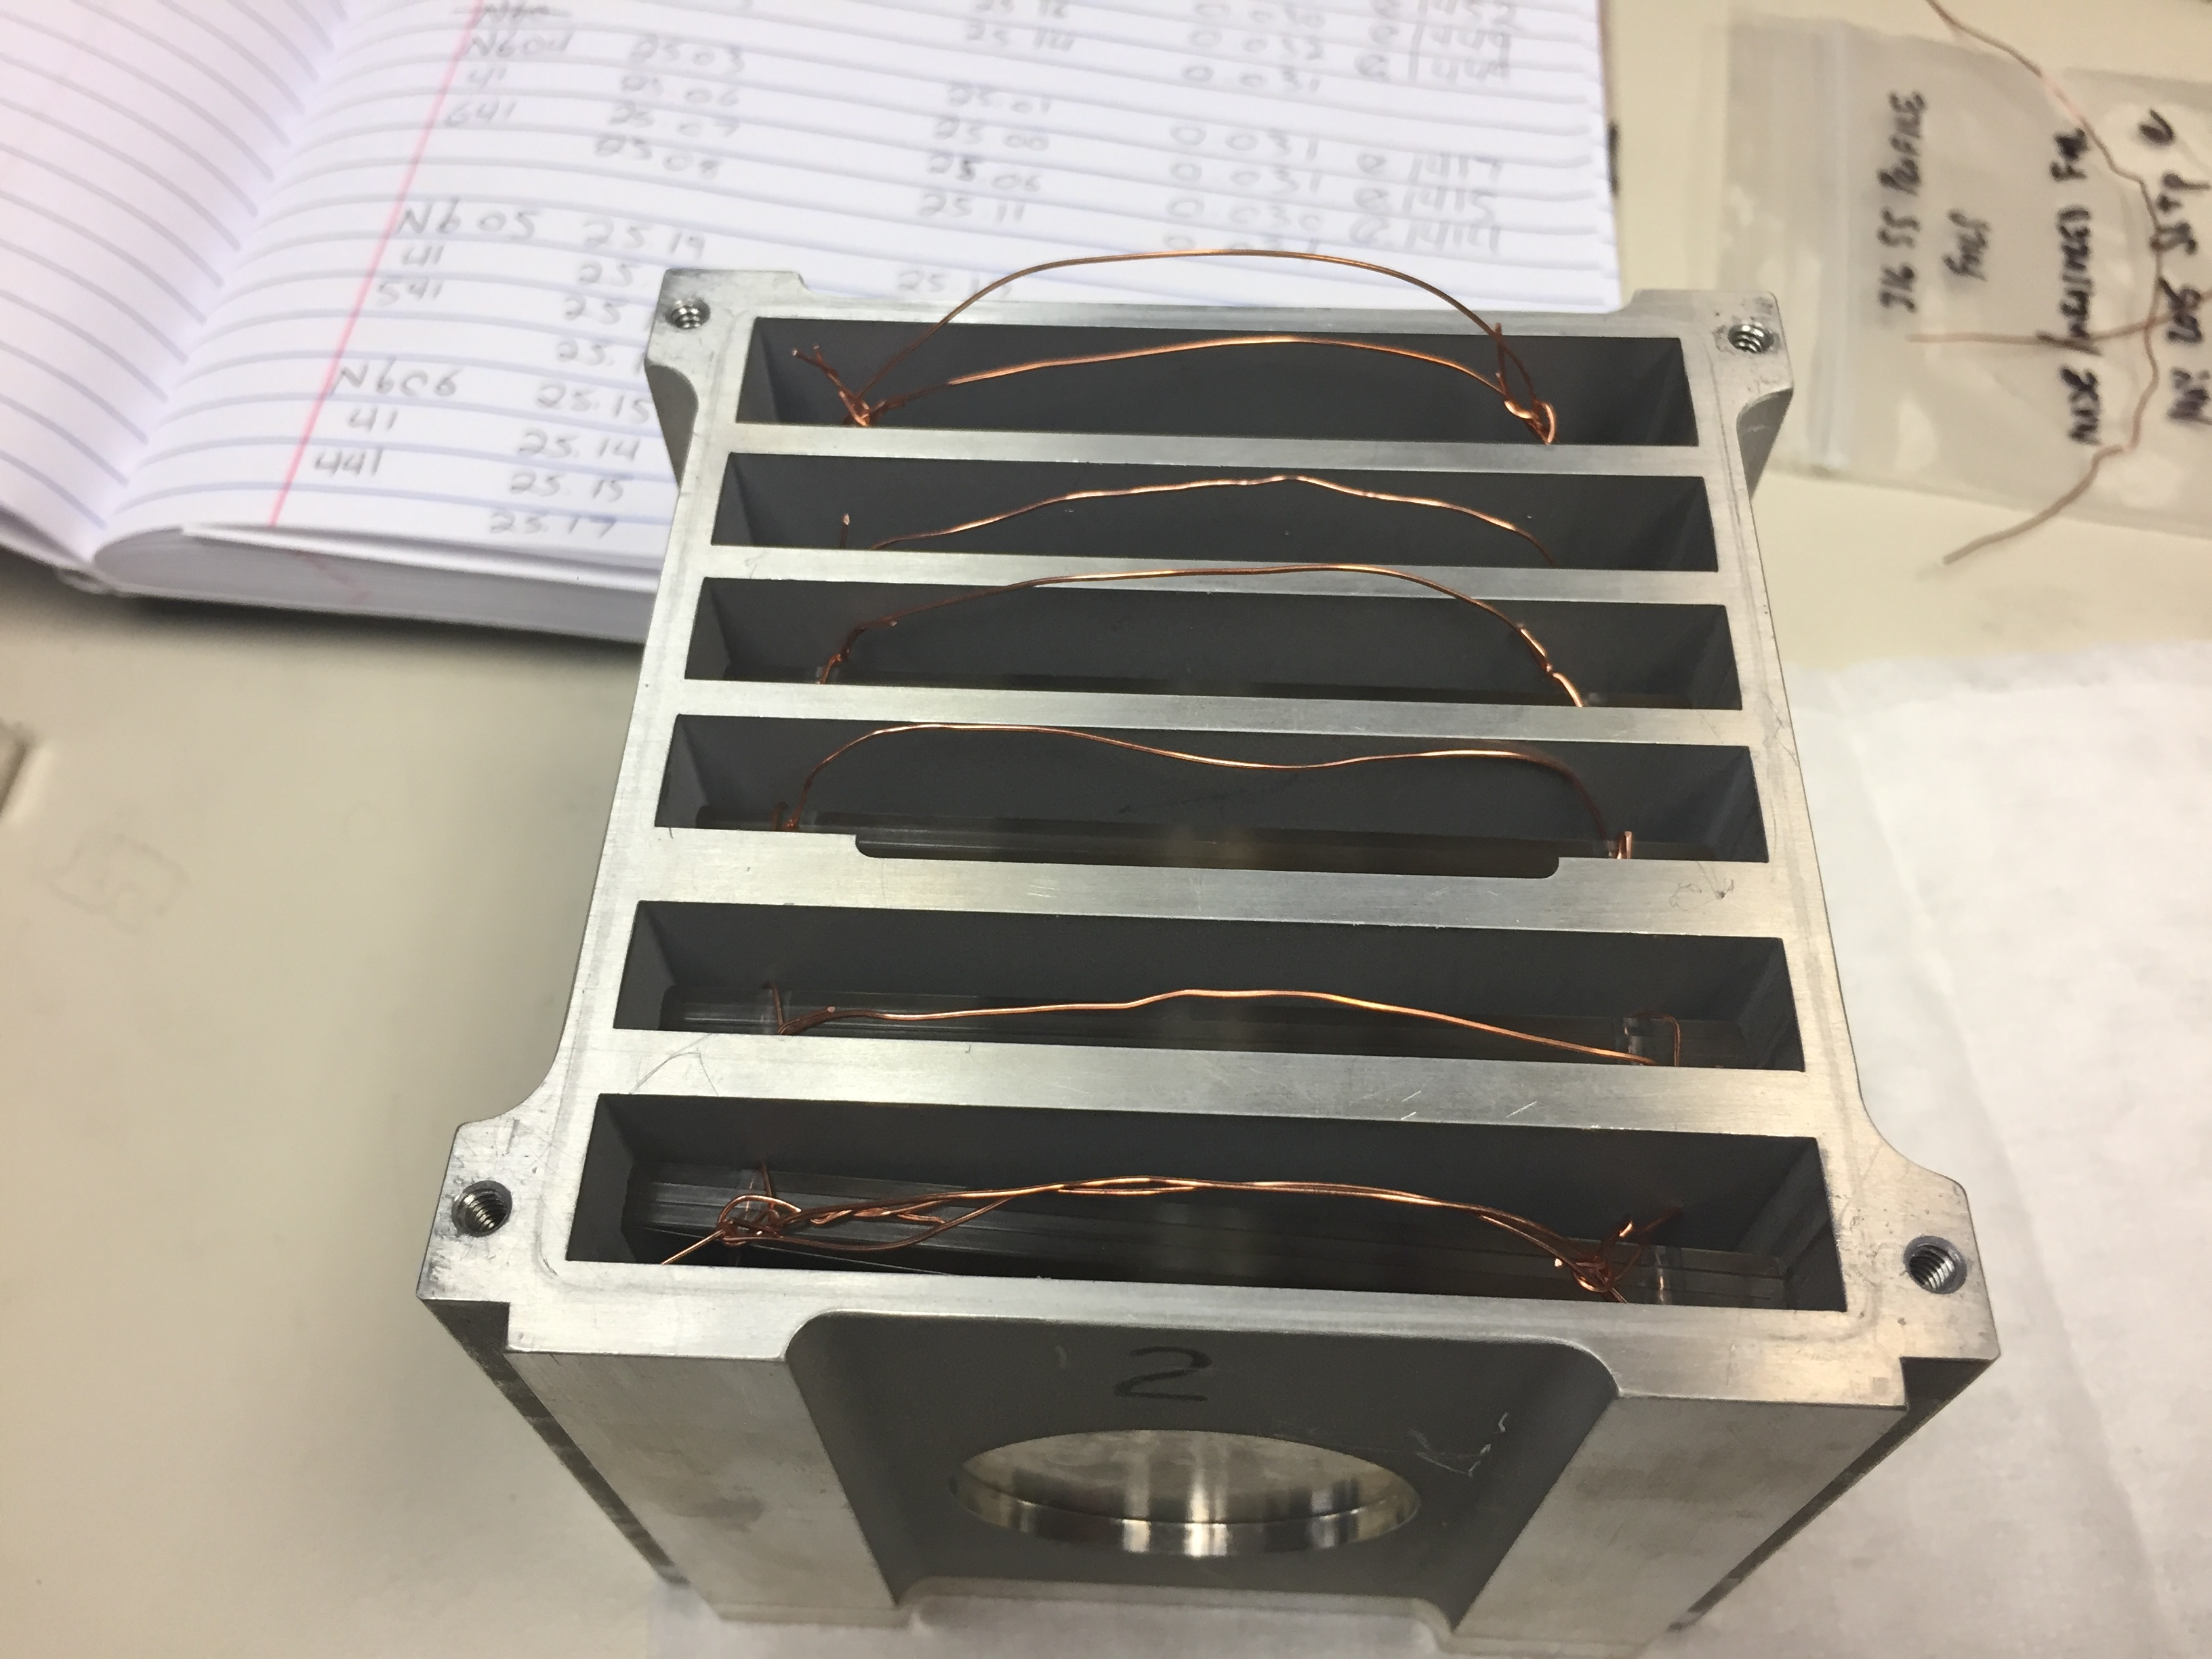
\includegraphics[width=0.5\linewidth,clip=true,trim=13cm 0cm 3cm 6cm]{./figures/IMG_1975.JPG}
 % IMG_1975.JPG: 3264x2448 pixel, 72dpi, 115.15x86.36 cm, bb=0 0 3264 2448
 \caption{\label{fig:target_stack}Photograph of the assembled IPF target stack, before the stack's o-ring lid was sealed in place. The baling wire handles affixed to each bunch of Al+Cu+Nb foils are visible in each energy position, to facilitate removal of activated foils via robotic manipulators in the IPF hot cell. The circular Inconel beam entrance aperture is visible in the bottom center of the photograph.  }
\end{figure}



% Please add the following required packages to your document preamble:
% \usepackage{booktabs}
\begin{table}
\centering
\caption{Specifications of the  target stack design in the present work. The proton beam enters the stack upstream of the 249.8 \micro m SS profile monitor, and is transported through the stack in the order presented here. The 6061 aluminum degraders have a measured density of approximately 2.80 g/cm$^3$. Their areal densities were determined using the variance minimization techniques described  in this work  and the earlier paper by Graves \etal \cite{Graves2016}}
\label{tab:stack_table}
\small
\begin{tabular}{@{}llll@{}}
\toprule
% Target Layer       & Nominal Thickness & Measured thickness (mg/cm\textasciicircum 2) & Thickness Uncertainty (\%) \\ \midrule
Target layer       & \begin{tabular}[c]{@{}l@{}}Measured \\ thickness\end{tabular} & \begin{tabular}[c]{@{}l@{}}Measured areal\\density (mg/cm$^2$)\end{tabular} & \begin{tabular}[c]{@{}l@{}}Areal density \\ uncertainty (\%)\end{tabular} \\ \midrule
SS profile monitor & 249.8 \micro m         & 194.56                                      & 0.29                      \\
Al-1               & 25.0 \micro m          & 6.52                                        & 0.72                      \\
Cu-1               & 61.3 \micro m          & 53.74                                       & 0.15                      \\
Nb-1               & 30.0 \micro m          & 23.21                                       & 0.17                      \\
Al Degrader 01     & 4.96 mm           & -                                            & -                          \\
Al-2               & 25.5 \micro m          & 6.48                                        & 0.36                      \\
Cu-2               & 61.8 \micro m          & 53.85                                       & 0.17                      \\
Nb-2               & 30.8 \micro m          & 22.91                                       & 0.17                      \\
Al Degrader 02     & 4.55 mm           & -                                            & -                          \\
Al-3               & 25.8 \micro m          & 6.47                                        & 0.31                      \\
Cu-3               & 61.5 \micro m          & 53.98                                       & 0.11                      \\
Nb-3               & 31.0 \micro m          & 22.91                                       & 0.24                      \\
Al Degrader 03     & 3.52 mm           & -                                            & -                          \\
Al-4               & 26.3 \micro m          & 6.51                                        & 0.41                      \\
Cu-4               & 61.3 \micro m          & 53.46                                       & 0.22                      \\
Nb-4               & 30.8 \micro m          & 22.55                                       & 0.25                      \\
Al Degrader 04     & 3.47 mm           & -                                            & -                          \\
Al-5               & 26.5 \micro m          & 6.48                                        & 0.29                      \\
Cu-5               & 61.5 \micro m          & 53.57                                       & 0.11                      \\
Nb-5               & 30.8 \micro m          & 22.11                                       & 0.25                      \\
Al Degrader 05     & 3.46 mm           & -                                            & -                          \\
Al-6               & 26.3 \micro m          & 6.48                                        & 0.62                      \\
Cu-6               & 62.0 \micro m          & 53.84                                       & 0.32                      \\
Nb-6               & 31.3 \micro m          & 22.12                                       & 0.13                      \\
SS profile monitor & 124.4 \micro m         & 101.34                                      & 0.23                      \\ \bottomrule
\end{tabular}
\end{table}





\subsection{Measurement of induced activities}\label{sec:spectroscopy}


For consistency, a single detector was used in this measurement, an ORTEC GEM Series (model \#GEM10P4-70)  High-Purity Germanium (HPGe) detector.
The detector is a mechanically-cooled coaxial p-type HPGe with a 1 mm aluminum window, and a 49.2 mm diameter, 27.9 mm long crystal.
Samples were counted at fixed positions ranging 4.5--83.5  cm (5\% maximum permissible dead-time) from the front face of the detector, with a series of standard calibration sources used to determine energy, efficiency, and pileup calibrations for each position.
The foils were counted  for a period of 2 weeks following EoB, to accurately quantify all induced activities,  with dead time never exceeding 5\%.
An example gamma-ray spectrum collected in such a fashion is shown in \autoref{fig:gspec}.
For all spectra collected, net peak areas were fitted using the gamma spectroscopy analysis code UNISAMPO \cite{Aarnio2001}, which has been shown to perform best in comparisons with other common analysis codes \cite{Jackman2014}.
%, due to its peak fitting algorithms and incorporation  of calibrated detector-specific peak shapes and widths. 

\begin{figure}
 \centering
 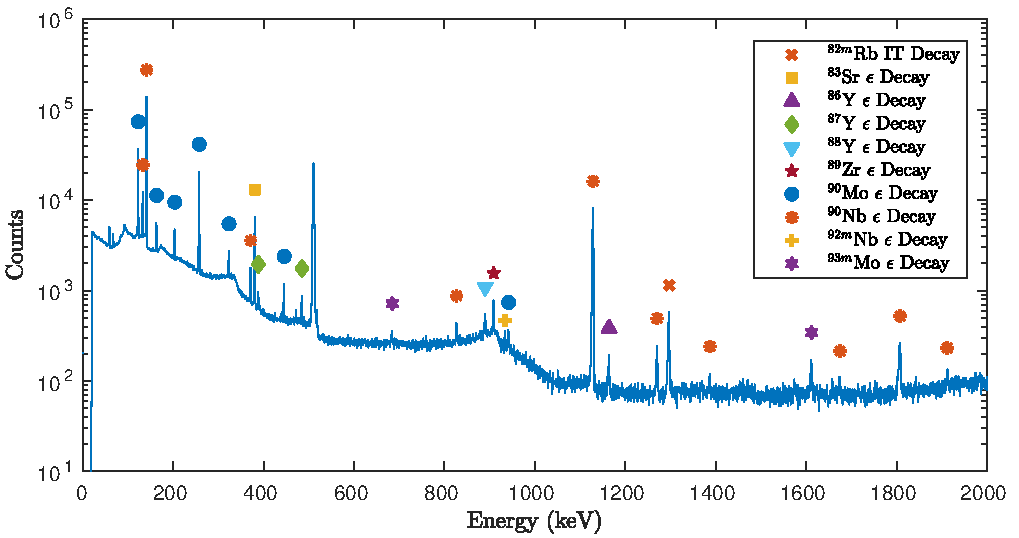
\includegraphics[width=6in]{./figures/sample_gspec.pdf}
 % sample_gspec.pdf: 489x257 pixel, 72dpi, 17.25x9.07 cm, bb=0 0 489 257
 \caption{A gamma spectrum, collected from an activated Nb foil at approximately 80 MeV. While the majority of observed reaction products are visible in this spectrum,  the \ce{^{90}Mo} decay lines, which form the basis of the \ce{^{93}Nb}(p,x)\ce{^{90}Mo} monitor reaction, are high in intensity and clearly isolated from surrounding peaks.}
 \label{fig:gspec}
\end{figure}


Following  acquisition, the decaying product nuclei corresponding to each observed peak in the collected spectra were identified.
The calibrated detector efficiencies, along with gamma-ray intensities for each transition and  corrections for gamma-ray attenuation within each foil packet, were used to convert the net  counts in each fitted gamma-ray photopeak into an activity for the decay of the activation products.  
For reference, the nuclear decay data used in this work is tabulated in \autoref{tab:nudat_table_monitors} and \autoref{tab:nudat_table_nb} of \ref{data}.
Data for photon attenuation coefficients are taken from the XCOM photon cross sections database  \cite{berger2011xcom}.
As nearly all of the product nuclei have multiple high-intensity gamma-rays, decay gamma-rays from the product nuclei were measured at multiple points in time (up to 2 weeks after EoB), as well as multiple independent activity measurements at each time point, based on each of its observed gamma-rays.
The measured activity for each gamma-ray possesses a total propagated uncertainty which is the quadrature sum of the uncertainty in  fitted peak areas, uncertainty in detector efficiency calibration, and uncertainty in the gamma-ray branching ratio data.






Since many of the reaction products populated by energetic protons are more than one decay off of stability, many of these are produced not only  directly by reactions, but also indirectly by decay down a mass chain.
To this end, it is useful to differentiate between the types of cross sections reported in this work. 
For the first observable product nuclei in a mass chain, its (p,x) cross section will be reported as a cumulative cross section ($\sigma_c$), which is the sum of direct production of that nucleus, as well as decay of its decay precursors and any other independent cross sections leading to that nucleus. 
In addition, cumulative cross sections will be reported whenever it is impossible to use decay spectroscopy to distinguish direct production of a nucleus from decay feeding.
For all remaining observed reaction products in the mass chain, and cases where no decay precursors exist, independent cross sections ($\sigma_i$) will be reported, allowing for determination of the direct production via subtraction.  



To convert these activities into cross sections, corrections must be made for the decay of the various reaction products during the time between EoB and the spectrum acquisition, in order to calculate $A_0$, the initial activity at EoB.
The use of  multiple gamma-rays at multiple points after EoB to calculate initial activities  for each observed product nucleus allows for a more accurate  determination of $A_0$ than simply basing its calculation off of a single gamma-ray observation.
For the case of cumulative cross sections, EoB activities were quantified by fitting the activities observed at multiple time points $t$ (since EoB) to the well-known radioactive decay law.
% \begin{equation}
% A\pp{t} = A_0 e^{-\lambda t}
% \end{equation}
Nonlinear regression was used for this fitting process, minimizing on $\chi^2$ / degree of freedom, so that not only would the uncertainty-weighted EoB activities be fitted, but that a 1-$\sigma$ confidence interval in $A_0$ would be reported as as well.
As with the gamma-ray intensities, all lifetimes used in this work are tabulated in \autoref{tab:nudat_table_monitors} and \autoref{tab:nudat_table_nb} of \ref{data}.
In the case of independent cross sections, a similar process was followed, quantifying $A_i\pp{t=0} = A_{i,0}$, the EoB activity of nuclide $i$, by instead regressing to the solutions to the Bateman equation \cite{bateman1910solution,Cetnar2006}:
\begin{equation}
A_n\pp{t} = \lambda_n \sum_{i=1}^n \left[  N_{i,0} \times \pp{\prod_{j=i}^{n-1}\lambda_j} \times \pp{\sum_{j=i}^n \dfrac{e^{-\lambda_j t}}{\prod_{i\neq j}^n \pp{\lambda_i - \lambda_j}}  }   \right]
\end{equation}
where $j$ refers to a precursor nucleus populating a specific end-product.  
While higher-order terms were added if needed, typically for an isomeric state in a particular mass chain,  the second-order expansion ($n=2$) was often sufficient to quantify EoB activities in a mass chain, simplifying to:
\begin{equation}
A_2\pp{t} = \dfrac{A_{1,0}\lambda_2}{\lambda_1 - \lambda_2} \pp{e^{-\lambda_2 t} - e^{-\lambda_1 t}} + A_{2,0} e^{-\lambda_2 t}
\end{equation}
In these cases, the previously-quantified EoB activities from decay precursors ($A_{1,0}$, etc) would be substituted in, so that the feeding contributions from decay could be separated and an independent cross section reported.
After quantifying the cumulative EoB activities at the top of a mass chain and all subsequent independent EoB activities, these will be later used to report the various cross sections for all observed reaction products and isomeric states. 











% \comment{Regex to replace table hard link with LaTeX cross-reference. - match w/ [T,t]able[^*}]   }


\subsection{Proton fluence determination}\label{sec:dosimetry}

% \comment{Stephen:  Still not a huge fan of the dosimetry terminology, but I would defer to the preference of those with more experience in the field. }

% describe integral equation for converting activities to currents here

An accurate integrated proton current is one of the most important factors in performing high-fidelity cross section measurements.
At the time of this work, the nondestructive beam current monitors in the LANSCE-IPF beamline had a  resolution of 100 nAh.
For a low-current irradiation such as this work, where a nominal fluence of 200 nAh is desired, additional fluence sensitivity is thus needed to accurately normalize quantified EoB activities into cross sections.
To this end, thin \ce{^{nat}Al} and \ce{^{nat}Cu} foils were included along with the \ce{^{nat}Nb} targets at each energy position, to provide another beam current monitor.
These foils have been recommended for use as proton monitor foils in the 30 \textless\ E$_\text{p}$ \textless\ 100 MeV regime by the IAEA, as the \ce{^{nat}Al}(p,x)\ce{^{22}Na}, \ce{^{nat}Al}(p,x)\ce{^{24}Na}, \ce{^{nat}Cu}(p,x)\ce{^{56}Co}, \ce{^{nat}Cu}(p,x)\ce{^{62}Zn}, and \ce{^{nat}Cu}(p,x)\ce{^{65}Zn} monitor reactions have been well-characterized for accurate proton fluence measurement \cite{gul2001charged}.
The recommended cross section values for each of these reactions were used in all calculations of proton fluence for the above monitor reactions.
Due to the large energy degradation between the front and  back of the target stack, a non-trivial broadening of the proton energy distribution is expected for all monitor and target foils.
As a result, the integral form of the well-known activation equation is used to accurately determine proton fluence ($I \Delta t $) in each monitor foil:
%by convolving the IAEA recommended cross section values with the proton energy distribution:
% \begin{equation}
% A_0 = I\ \rho \Delta r \pp{1-e^{-\lambda \Delta t}} \int \sigma\pp{E} \dfrac{d\phi}{dE} dE
% \end{equation}
\begin{equation}
I \Delta t = \dfrac{A_0 \Delta t}{\rho \Delta r \pp{1-e^{-\lambda \Delta t}} \int \sigma\pp{E} \dfrac{d\phi}{dE} dE}
\end{equation}
where $A_0$ is the EoB activity for the monitor reaction product, $I$ is the proton current, $\rho \Delta r$ is the foil's areal density, $\lambda$ is the monitor reaction product's decay constant, $\Delta t$ is the length of irradiation, $\sigma\pp{E}$ is the IAEA recommended cross section at energy $E$, and $\frac{d\phi}{dE}$ is the differential proton fluence.
Using this formalism, the quantified EoB activities for each monitor reaction may be converted into a measured proton fluence at each energy position.



The propagated uncertainty in proton fluence is calculated as the quadrature sum of the uncertainty in quantified EoB activity, uncertainty in the duration of irradiation (conservatively estimated at 60 s, to account for any transient changes in beam current), uncertainty in foil areal density, uncertainty in monitor product half-life (included, but normally negligible), uncertainty in IAEA recommended cross section, and uncertainty in differential proton fluence.
Of these, the first four contributions are all easily quantified in the preparation and execution of a stacked target irradiation;  the last two contributions prove to be more nuanced, however.
The uncertainty in proton fluence for irradiated monitor foils is derived from statistical uncertainty in the modeling of proton transport in the stack irradiation, discussed in \autoref{sec:proton_transport}.
The uncertainty in IAEA recommended cross section values must be estimated indirectly, as no uncertainty in the  recommended cross sections is provided in the current IAEA evaluation.
Fortunately, the recommended cross section values for each monitor reaction tend to closely match one of the   selected experimental data sets used in their evaluation.
Since these data sets have listed uncertainties in the original manuscripts, uncertainties in  IAEA recommended cross section values have been estimated by the uncertainty in the data set most closely matching the  IAEA recommended  values.
For the monitor reactions employed in this work, these data sets are G. Steyn (1990) for  \ce{^{nat}Al}(p,x)\ce{^{22}Na} \cite{Steyn1990}, M. Uddin (2004) for \ce{^{nat}Al}(p,x)\ce{^{24}Na} \cite{Uddin2004}, and S. Mills (1992) for \ce{^{nat}Cu}(p,x)\ce{^{56}Co}, \ce{^{nat}Cu}(p,x)\ce{^{62}Zn}, and \ce{^{nat}Cu}(p,x)\ce{^{65}Zn} \cite{Mills1992}.




\subsection{Proton transport calculations}\label{sec:proton_transport}


Initial estimates of the proton beam energy in all foils were calculated using the Anderson \& Ziegler (A\&Z) stopping power formalism \cite{Andersen_Ziegler_1977,Ziegler1985,Ziegler1999}.
These estimates of average beam energy in each foil are useful for the preliminary stack design, as the A\&Z calculations provide reasonable approximations of 1-D proton transport due to treatment of ionization and multiple Coulomb scattering. 
However, for final energy and fluence determinations, a more rigorous method of proton transport is needed.
The Monte Carlo N-Particle transport code MCNP6.1 was used for simulation of the full 3-D target stack, including determination of the full proton energy distribution for each stack position   \cite{Goorley2012}.
In addition, MCNP6 provides a far more robust method of proton transport, as it is able to account for beam losses due to scattering and reactions, as well as production of secondary particles.
As it is a Monte Carlo-based code, the uncertainty in energy distribution scales inversely with the number of source protons simulated.  $10^8$ source protons were used for all simulations, which places the statistical uncertainty in proton energy distributions at less than 0.01\%.


The ability to model the full energy distribution in each target position is vital for stacked target irradiations, due to the progressively larger energy straggling towards the rear of the stack.
The initial proton beam has a finite energy spread (an approximately 0.1 MeV Gaussian width at 100 MeV), and since stopping power for charged particles is inversely proportional to their energy, the low-energy tail of the energy distribution is degraded more in each stack element than the high-energy tail.
This effect compounds  towards the rear of the stack, creating a significantly broadened low-energy tail, and a progressively larger net shift of the centroid to a lower energy. 
% For each foil in the target stack, 
To account for this increasing energy uncertainty, a suitably representative energy must be established for  each foil in the target stack.
In this work, the flux-weighted average proton  energy in each foil, $\langle E \rangle$,  represents the energy centroid for protons in a target stack component, calculated using the energy distributions $\frac{d\phi}{dE}$ from MCNP6 modeling of proton transport:
\begin{equation}
\langle E \rangle = \dfrac{{\displaystyle\int E \dfrac{d\phi}{dE} dE}}{{\displaystyle\int \dfrac{d\phi}{dE} dE}}
\end{equation}
Likewise, to represent the energy uncertainty for each stack position, the full width at half maximum (FWHM) of the MCNP6-modeled energy distribution is chosen for each energy position reported.
While most experimental uncertainties are reported at the 1$\sigma$ level, the $\approx2.3\sigma$ FWHM is used here to ensure at the 98\% confidence interval that this width includes  the \enquote{true} energy centroid value.





The \enquote{variance minimization} techniques  described by  Graves \etal\  have been employed here to further reduce the uncertainty in proton energy assignments     \cite{Graves2016}.
This method is based on the assumption that the independent measurements of proton fluence from the 5 monitor reactions used in this work should all be consistent at each energy position.
If the monitor reaction cross sections and MCNP6-modeled energy distributions are both accurate, then any disagreement in the  observed proton fluences is due to a systematic uncertainty in the stack design, namely, the areal densities of the stack components \cite{Graves2016,Marus2015}. 
This disagreement is minor at the front of the stack, and gets progressively worse as the beam is degraded, due to the compounded effect of systematic uncertainties in stack areal densities.



Variance minimization techniques were employed  to correct for uncertainties in  the characterization of the stack components, the largest cause of uncertainties in energy and  fluence assignments.
Due to the difficulty of characterizing uncertainty in areal density in the Kapton tape, the areal density of these layers were varied uniformly in MCNP6 simulations by up to $\pm$25\% of nominal values.
This had negligible impact on improving monitor reaction disagreement  due to the small effect that their areal density has on beam degradation relative to the thick 6061 aluminum degraders (nominal 3--5 mg/cm$^2$, relative to nominal 1000--1400 mg/cm$^2$).
As such,  the areal density of each of the 6061 aluminum degraders  were varied uniformly in MCNP6 simulations  by a factor of up to $\pm$25\% of nominal values, to find the effective density which minimized variance in the measured proton fluence at the lowest energy position (Al-6, Cu-6).
This lowest energy position was chosen as a minimization candidate, as it is most sensitive to systematic uncertainties in stack design.
The results of this minimization technique, shown in \autoref{fig:variation_curve}, indicate a clear minimum in proton fluence variance for flux-weighted average 41.34 MeV protons entering the last energy position.
This is approximately 2 MeV lower than the nominal MCNP6 simulations, and approximately 3 MeV lower than nominal A\&Z calculations, both of which used the nominal 2.80 g/cm$^3$ measured density of the 6061 aluminum degraders.
This energy corresponds to a 6061 aluminum areal density of 2.52\% greater than nominal measurements, and serves as a lump correction for other minor systematic uncertainties in stack design, including stack areal densities and incident beam energy.




\begin{figure}
 \centering
%  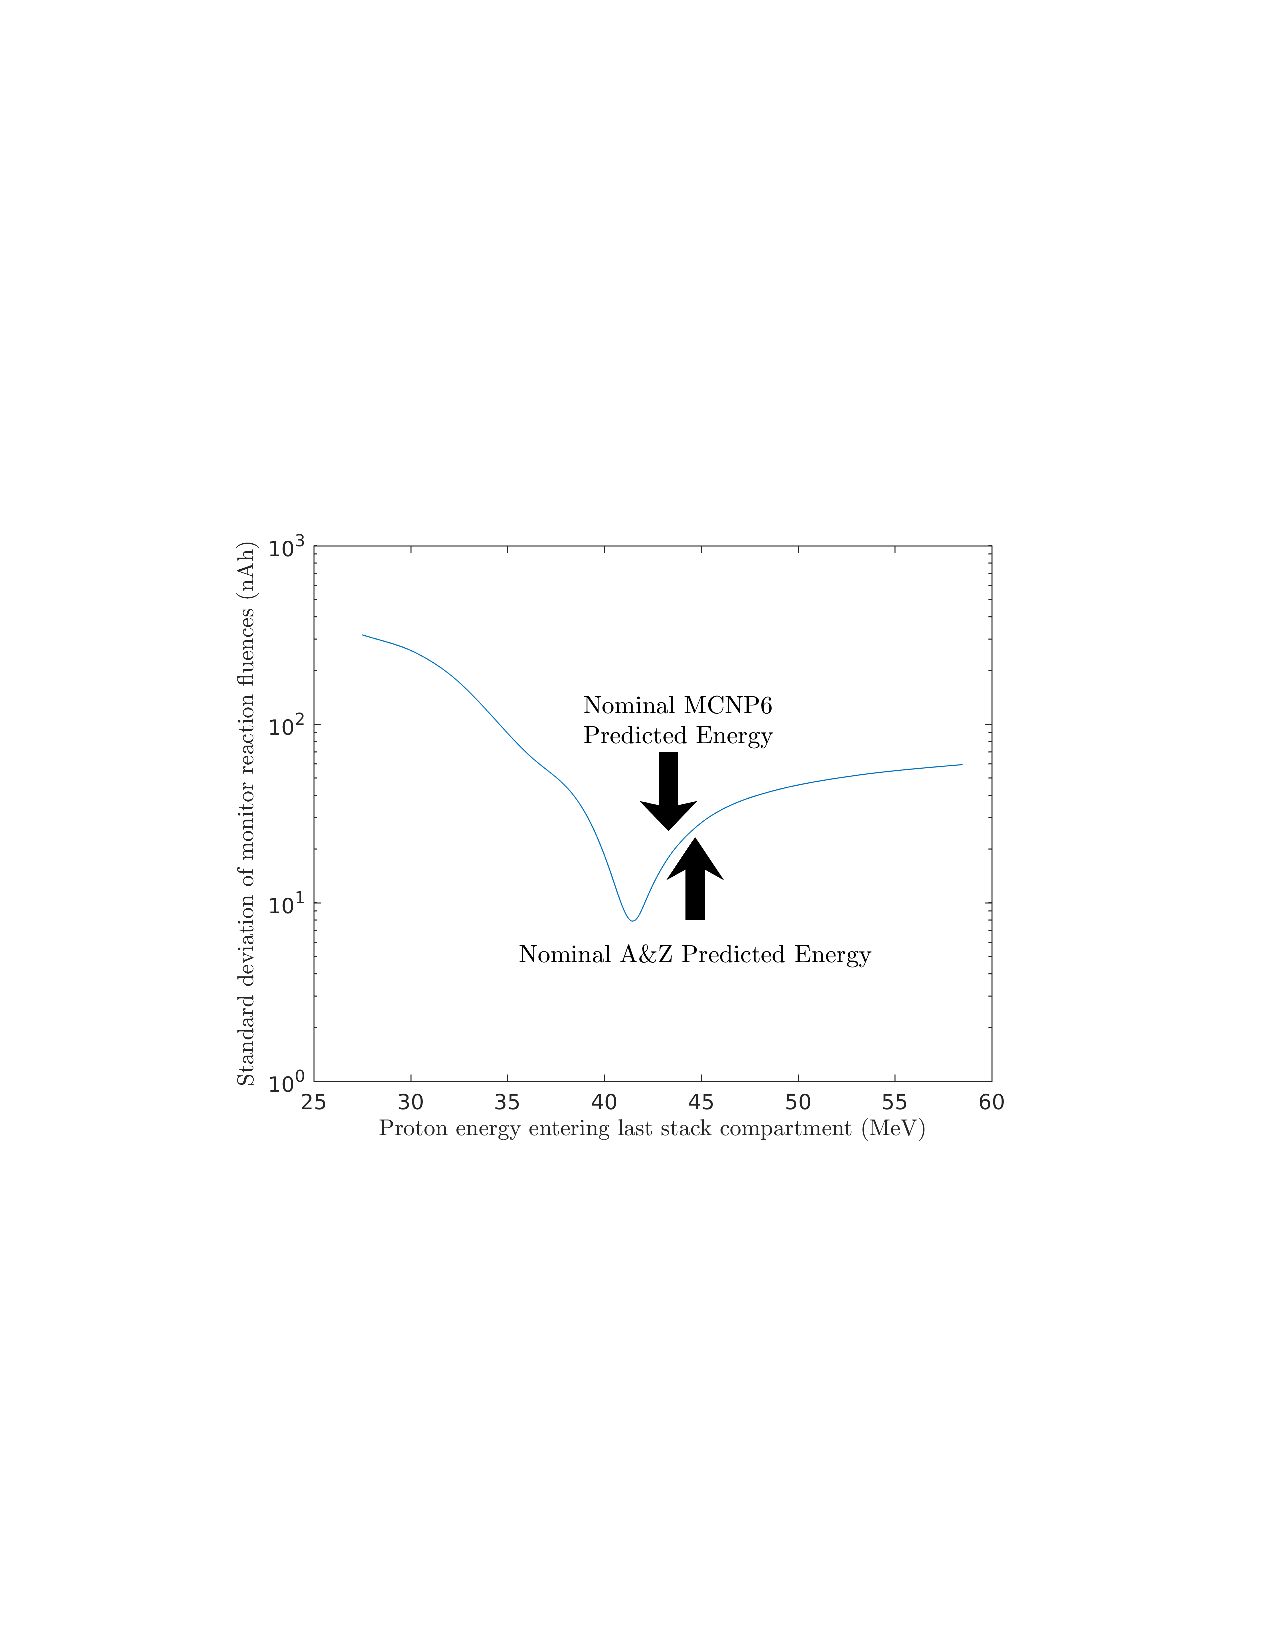
\includegraphics[clip=true,trim=1.5in 3.4in 1.8in 3.5in, scale=0.8]{./figures/variation_curve.pdf}
 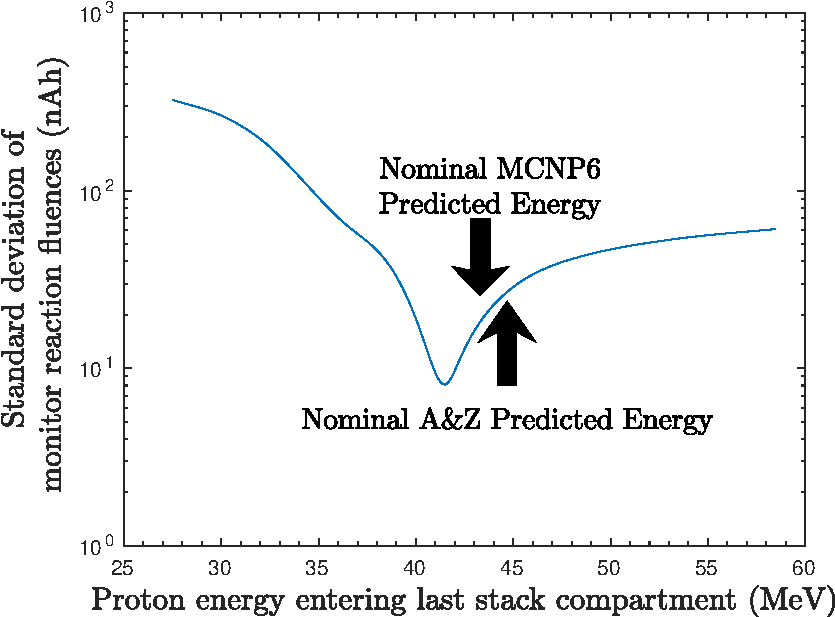
\includegraphics[width=0.5\linewidth]{./figures/variation_curve-crop.pdf}

 % variation_curve.pdf: 612x792 pixel, 72dpi, 21.59x27.94 cm, bb=0 0 612 792
 \caption{Result of the variance minimization performed by adjusting the degrader density in MCNP6 simulations of the target stack.  A flux-weighted average proton energy of 41.34 MeV entering the last energy position creates a clear minimum in observed reaction fluence variance, corresponding to an areal density 2.52\% greater than nominal. The variance minimum occurring at a lower incident energy than nominal MCNP6 and A\&Z calculations indicates that there exists an additional systematic beam degradation not accounted for in modeling of proton transport in the stack design.}
 \label{fig:variation_curve}
\end{figure}


\begin{figure}
    \centering
    \begin{subfigure}[t]{0.50\textwidth}
        \centering
%         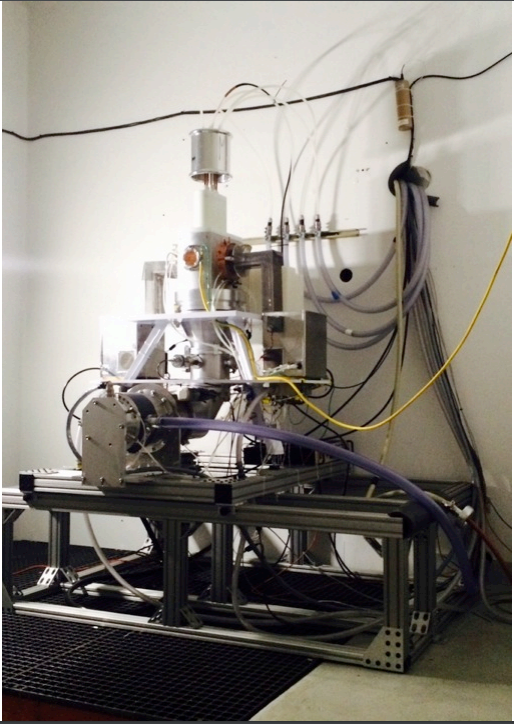
\includegraphics[width=\columnwidth]{./figures/Capture.PNG}
        \subfigimg[width=\linewidth]{a)}{./figures/before_minimization_plot.pdf}{50}
%         \caption{ Decay curve for the isomeric transition of \ce{^{115m}In}.}
         \refstepcounter{subfigure}\label{fig:before_minimization}
    \end{subfigure}%
     \begin{subfigure}[t]{0.50\textwidth}
        \centering
%         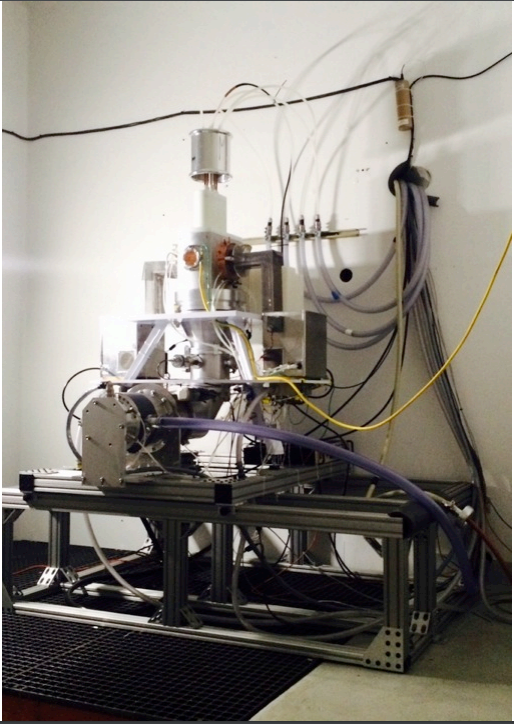
\includegraphics[width=\columnwidth]{./figures/Capture.PNG}
%         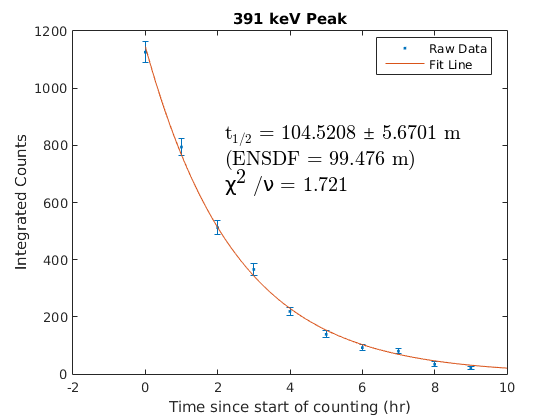
\includegraphics[scale=0.6]{./figures/391keV_curve2.png}
        \subfigimg[width=\linewidth]{b)}{./figures/after_minimization_plot.pdf}{50}
%         \caption{ Decay curve for the isomeric transition of \ce{^{113m}In}.}
         \refstepcounter{subfigure}\label{fig:after_minimization}
    \end{subfigure}%
    \caption{Results of variance minimization through enhancement of the effective areal density of the 6061 aluminum degraders by 2.52\%. A noticeable reduction of variance in measured proton fluence is seen,  particularly at the  rear stack positions. Following minimization, additional apparent fluence is observed in the  \ce{^{nat}Al}(p,x)\ce{^{22}Na} and \ce{^{nat}Al}(p,x)\ce{^{24}Na} monitor channels, due to contamination from \ce{^{nat}Si}(p,x)\ce{^{22,24}Na} on the silicone adhesive used for sealing foil packets.}
     \label{fig:variance_mins}
\end{figure}

\begin{figure}
    \centering
    \begin{subfigure}[t]{0.50\textwidth}
        \centering
%         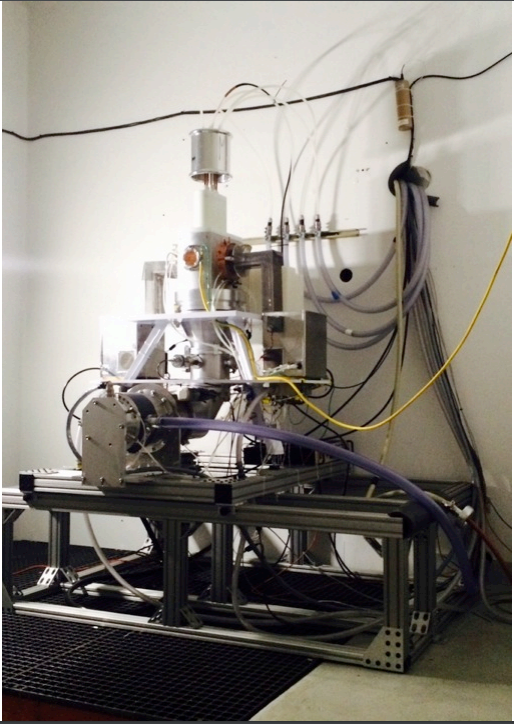
\includegraphics[width=\columnwidth]{./figures/Capture.PNG}
        \subfigimg[width=\linewidth]{a)}{./figures/Na22_activity_compare.pdf}{50}
%         \caption{ Decay curve for the isomeric transition of \ce{^{115m}In}.}
         \refstepcounter{subfigure}\label{fig:Na22_activity_compare}
    \end{subfigure}%
     \begin{subfigure}[t]{0.50\textwidth}
        \centering
%         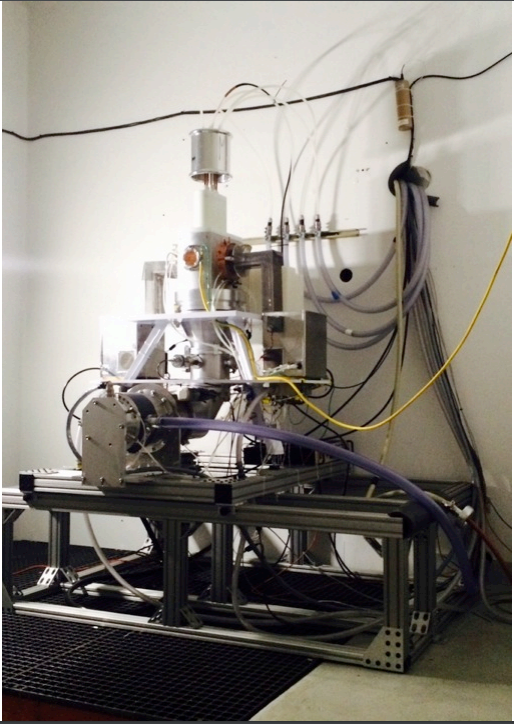
\includegraphics[width=\columnwidth]{./figures/Capture.PNG}
%         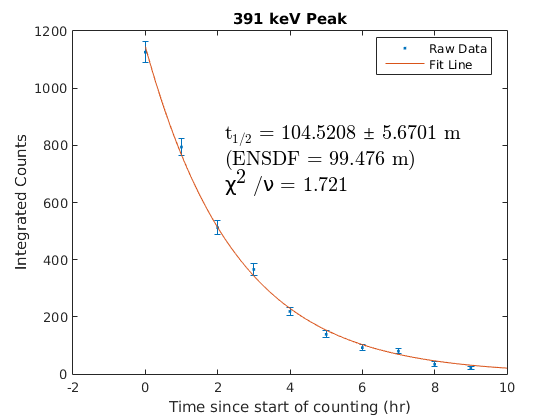
\includegraphics[scale=0.6]{./figures/391keV_curve2.png}
        \subfigimg[width=\linewidth]{b)}{./figures/Na24_activity_compare.pdf}{180}
%         \caption{ Decay curve for the isomeric transition of \ce{^{113m}In}.}
         \refstepcounter{subfigure}\label{fig:Na24_activity_compare}
    \end{subfigure}%
    \caption{Estimates of EoB \ce{^{nat}Al}(p,x)\ce{^{22,24}Na} and \ce{^{nat}Si}(p,x)\ce{^{22,24}Na} activities using TENDL-2015 cross sections, in comparison with the IAEA recommended \ce{^{nat}Al}(p,x)\ce{^{22,24}Na} cross sections. At low energies, experimentally observed apparent \ce{^{22,24}Na} activities in each Al foil packet are consistent with IAEA recommendations, but diverge at higher energies as the \ce{^{nat}Si}(p,x)\ce{^{22}Na} exit channels begin to open up. \ce{^{22,24}Na} activities consistent with TENDL-2015 estimates are observed in each Nb and Cu foil packet as well, confirming that contamination may be attributed to activation of silicone adhesives.}
     \label{fig:Na_activity_compare}
\end{figure}



The impact of this variance minimization may  clearly be seen in   \autoref{fig:variance_mins}.
As expected, the 2.52\% increase in 6061 aluminum areal density has an almost negligible impact on the higher-energy positions, but causes a progressively larger downshift  in proton energies at the later energy positions.
In addition, as one moves to the rear  positions, the disagreement in the independent proton fluence measurements is reduced.
% \comment{Insert text here to describe our Na22 / Si production hypothesis.  }
It is worth noting that the proton fluence measured by the \ce{^{nat}Al}(p,x)\ce{^{22}Na} monitor reaction (threshold 21.0 MeV) is consistently higher in magnitude than all other monitor channels, with an increasing disparity at higher energies.
This phenomenon is observed for the \ce{^{nat}Al}(p,x)\ce{^{24}Na} monitor reaction as well (threshold 24.6 MeV), though to a much smaller degree.
In both cases, this disparity is caused by the fact that the Kapton tape used for sealing foil packets (comprised of a silicone adhesive layer on a polyimide backing) contains a significant amount of silicon, making up approximately 10\% of the silicone on a stoichiometric basis.
\ce{^{22}Na} and \ce{^{24}Na}, the residual nuclei used as monitors, can also be populated off of natural silicon  (92.2\% \ce{^{28}Si}), predominantly via \ce{^{28}Si}(p,$\alpha$2pn)\ce{^{22}Na} (threshold 35.3 MeV) and \ce{^{28}Si}(p,4pn)\ce{^{24}Na} (threshold 44.6 MeV).
\ce{^{29}Si} and \ce{^{30}Si} are also potential targets for (p,x)\ce{^{22,24}Na}, albeit with higher energetic thresholds and smaller cross sections.
In addition, each aluminum foil packet contains approximately 6.5 mg/cm$^2$ of Al, as well as approximately  9.6 mg/cm$^2$ of silicone.
The attribution of excess Al(p,x)\ce{^{22,24}Na} activity to the silicone adhesive is confirmed by the observation of \ce{^{22}Na} and \ce{^{24}Na} activities in all Cu and Nb foil positions.



These compensating factors  contribute to \ce{^{28}Si}(p,$\alpha$2pn)\ce{^{22}Na} production being competitive with the \ce{^{nat}Al}(p,x)\ce{^{22}Na} production route.
This is made made obvious when comparing the total measured activities of \ce{^{22}Na} and \ce{^{24}Na} in each Al foil packet (which combines both Al- and Si-based production routes), relative to the expected EoB activities for each reaction channel, presented in \autoref{fig:Na_activity_compare}.
Since no evaluated  cross section data exists in this energy region  for  \ce{^{28}Si}(p,x)\ce{^{22}Na}  (and only minimal \ce{^{nat}Si} data exists),  the TENDL-2015 library is used to estimate the expected relative EoB activities for \ce{^{nat}Al}(p,x)\ce{^{22,24}Na} and \ce{^{nat}Si}(p,x)\ce{^{22,24}Na}, in comparison with the IAEA recommended \ce{^{nat}Al}(p,x)\ce{^{22,24}Na} cross sections.
Several observations are immediately obvious.
At lower energies, the magnitude of \ce{^{nat}Al}(p,x)\ce{^{22}Na} is large compared to \ce{^{nat}Si}(p,x)\ce{^{22,24}Na}, which is why the \ce{^{nat}Al}(p,x)\ce{^{22}Na} monitor agrees in fluence at the 40 (and almost at the 50) MeV position.  
At higher energies, the apparent \ce{^{nat}Al}(p,x)\ce{^{22}Na} activity begins to diverge from the IAEA expected activities as     \ce{^{nat}Si}(p,x)\ce{^{22}Na} production begins to open up,  which accounts for the nearly 50\% apparent excess fluence in \ce{^{22}Na} between 60--90 MeV.
For the \ce{^{24}Na} production, we see a similar behavior, though since the observed \ce{^{nat}Si}(p,x)\ce{^{24}Na} yield remains consistently low in magnitude, only a minor increase in apparent \ce{^{24}Na} activity is seen.
The measured EoB \ce{^{22}Na} and \ce{^{24}Na} activities seen  in all Cu and Nb foil positions are also shown here, which are seen to be consistent with the TENDL-2015 \ce{^{nat}Si}(p,x)\ce{^{22}Na} yields. 
The observed \ce{^{24}Na} activities also follow the shape of the TENDL-2015 \ce{^{nat}Si}(p,x)\ce{^{24}Na} yields, albeit smaller in magnitude at the higher energy positions.




While these TENDL cross sections simply provide approximate \ce{^{nat}Si}(p,x)\ce{^{22,24}Na} yields,  there are several important  conclusions to be drawn from this quick estimate.
The observation of the \ce{^{22,24}Na} activities in Cu and Nb foils  represents an indirect measurement of the \ce{^{nat}Si}(p,x)\ce{^{22,24}Na} cross sections, but they will not be reported due to the number of assumptions involved in such a calculation.
The EoB \ce{^{22,24}Na} activities have been measured directly, but to convert these into absolute cross sections, accurate knowledge of the precise silicone composition and areal density are required.
These have been taken as 10\% (stoichiometric basis) and 4.79 mg/cm$^2$ (based on bulk density), respectively, for the purposes of transport calculations, but this level of confidence is insufficient for the reporting of a cross section.
In principle, it would be possible  to subtract out the measured \ce{^{22,24}Na} activity at each Nb and Cu foil position (correcting for the minor difference in proton energy between adjacent foils) from the total \ce{^{22,24}Na} apparent activities observed in each Al foil packet, in order to obtain the \enquote{true} or uncontaminated fluence via the aluminum monitor reactions.
The results of this  may be seen in \autoref{fig:na_subtraction} --- following subtraction, the \ce{^{22,24}Na} fluences become consistent with other monitor reaction channels, within a mere 3--4\% spread.
While this would circumvent the assumptions needed for reporting \ce{^{nat}Si}(p,x)\ce{^{22,24}Na} cross sections, subtraction of  inaccurately quantified \ce{^{22,24}Na} activity in each Nb and Cu foil would propagate into the final fluence determination at each energy position, shifting the magnitude of all reported cross sections.
Even following subtraction, the \ce{^{22}Na} fluence remains 3--6\% higher than the weighted mean of the remaining monitor reaction channels.
While the dramatic improvement in monitor reaction consistency builds confidence, in the interest of surety and because they are consistent, only the \ce{^{nat}Cu}(p,x)\ce{^{56}Co}, \ce{^{nat}Cu}(p,x)\ce{^{62}Zn}, and \ce{^{nat}Cu}(p,x)\ce{^{65}Zn} monitor reaction channels will be used for fluence determination for the reported cross sections.
% In both cases, this disparity is caused by the fact that both of these monitor reactions may also form the \ce{^{22}Na} and \ce{^{56}Co} reaction products through contamination by secondary neutron (n,x) channels, increasing the apparent fluence as observed by these monitor reactions.
% Since no method for reliably separating the fraction of \ce{^{22}Na} and \ce{^{56}Co} activities induced through (n,x) exists, the fluences predicted by these monitor channels are not used in the final determination of the proton fluence seen by Nb foils. 
% The fact that this \enquote{extra fluence} diminishes at lower energy is likely attributed to the fact that the \ce{^{nat}Al}(p,x)\ce{^{22}Na} and \ce{^{nat}Cu}(p,x)\ce{^{56}Co} have energetic thresholds of 23.35 and 36.76 MeV, respectively. 
% The fraction of secondary neutrons produced by (p,xn)  which are energetic enough to populate the  \ce{^{22}Na} and \ce{^{56}Co} reaction products at the lower energy positions becomes progressively smaller.
This serves as a pointed example of the importance of selecting monitor reaction products inaccessible through channels aside from the primary reaction (\ce{^{nat}Al}(p,x)\ce{^{22,24}Na}, in this case ), as noted previously.
% However,  the fact that both monitor reactions measure consistently higher fluence than the other channels on each foil builds confidence that the monitor reactions accurately indicate the presence of a non-negligible secondary neutron flux.


% Avoud using al and silicone






\begin{figure}
    \centering
    \begin{subfigure}[t]{0.50\textwidth}
        \centering
%         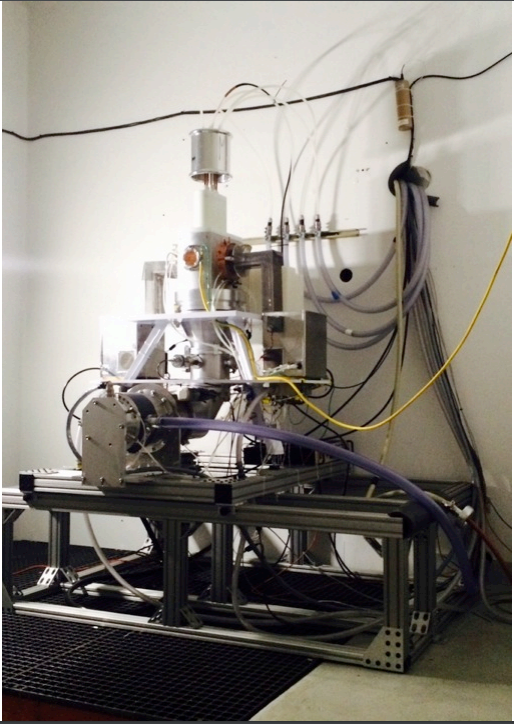
\includegraphics[width=\columnwidth]{./figures/Capture.PNG}
        \subfigimg[width=\linewidth]{a)}{./figures/after_minimization_plot_alt.pdf}{80}
%         \caption{ Decay curve for the isomeric transition of \ce{^{115m}In}.}
         \refstepcounter{subfigure}\label{fig:before_subtraction}
    \end{subfigure}%
     \begin{subfigure}[t]{0.50\textwidth}
        \centering
%         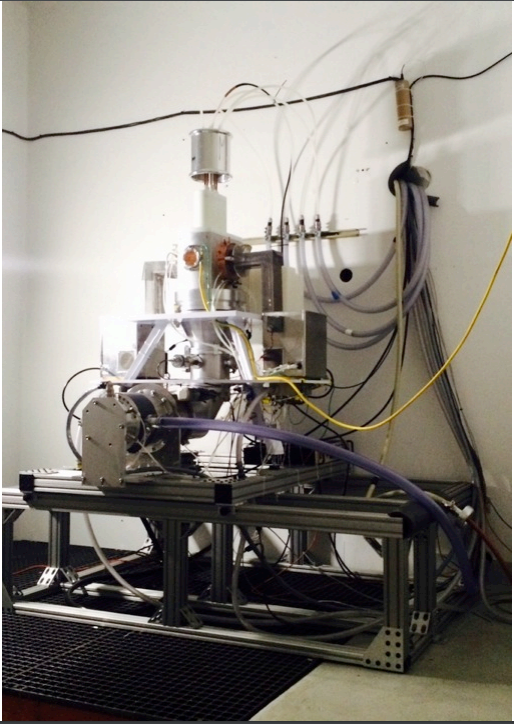
\includegraphics[width=\columnwidth]{./figures/Capture.PNG}
%         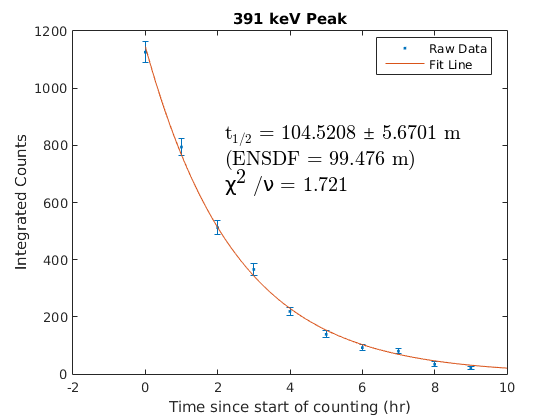
\includegraphics[scale=0.6]{./figures/391keV_curve2.png}
        \subfigimg[width=\linewidth]{b)}{./figures/after_subtraction_plot.pdf}{80}
%         \caption{ Decay curve for the isomeric transition of \ce{^{113m}In}.}
         \refstepcounter{subfigure}\label{fig:after_subtraction}
    \end{subfigure}%
    \caption{The \enquote{extra fluence} observed in the  \ce{^{nat}Al}(p,x)\ce{^{22}Na} and \ce{^{nat}Al}(p,x)\ce{^{24}Na} monitor channels is caused by contamination from \ce{^{nat}Si}(p,x)\ce{^{22,24}Na} on the silicone adhesive used for sealing foil packets. Following subtraction of \ce{^{22,24}Na} activities observed in the silicone adhesive of Nb and Cu foils in the same energy \enquote{compartment}, the consistency of the \ce{^{nat}Al}(p,x)\ce{^{22}Na} monitor reaction improves  dramatically.  By excluding these contaminated channels, the remaining 3 independent monitor reactions serve to minimize uncertainty in stack energy assignments and incident fluence.}
     \label{fig:na_subtraction}
\end{figure}

Using this variance minimized degrader density, the final incident proton energy energy distributions $\frac{d\phi}{dE}$ from MCNP6 simulation are shown for the 6 irradiated Nb foils in \autoref{fig:Nb_ptallies}. 
As expected, the energy distribution becomes increasingly more broadened at the lower energy positions, as a result of the beam energy degradation.
In addition, as the beam becomes more degraded, the magnitude of the peak of each energy distribution (as well as the integral of each distribution) is reduced in magnitude, as beam fluence is lost due to scattering, and the peak-to-low-energy-tail ratio increases as more  secondary protons are produced upstream.
As with the monitor foils, these distributions were used to calculate the  energy centroid  (as the  flux-weighted average proton  energy) and  uncertainty (as the FWHM of the distribution) for the final proton energy assignment of each Nb foil.





An enhanced version of the final monitor reaction fluences may be seen in \autoref{fig:fluence_plot}, which shows the   observed fluence of the \ce{^{nat}Cu}(p,x)\ce{^{56}Co}, \ce{^{nat}Cu}(p,x)\ce{^{62}Zn}, and \ce{^{nat}Cu}(p,x)\ce{^{65}Zn} monitor reaction channels.
Without the reliable use of the  \ce{^{nat}Al}(p,x)\ce{^{22}Na} and \ce{^{nat}Al}(p,x)\ce{^{24}Na} monitor channels, local interpolation cannot be used for fluence assignment to the Nb foils, and global interpolation is reliant upon a validated model for fluence loss.
In the interest of surety of because they are consistent, the uncertainty-weighted mean  for the three \ce{^{nat}Cu}(p,x) monitor channels was calculated at each energy position, to determine the final fluence assignments for the Nb and Cu foils.
Uncertainty in proton fluence  is likewise calculated as the error propagation of the fluence values  at each energy position.
These weighted-mean fluences are also plotted in in \autoref{fig:fluence_plot}, along with the estimated fluence according to both the MCNP6 transport model, as well as an uncertainty-weighted linear $\chi^2$ fit to the individual  fluence measurements in each monitor channel.
Both models reproduce the observed fluence data consistently within uncertainty, with the MCNP6 model predicting a slightly more aggressive fluence loss throughout the stack.
These models are used purely to provide an extrapolation from the 90 MeV energy position back to the \enquote{front} of the stack at 100 MeV, to compare with the nominal fluence measured by the IPF upstream current monitors.
% This involved minimizing on $\chi^2$ / degree of freedom, so that  a 95\% confidence interval in fluence would be reported as as well.
% As with the FWHM, a greater than 1$\sigma$ confidence interval is used for reporting fluence uncertainty to avoid an unrealistically small fluence confidence interval, based on the spread in observed fluence from Al and Cu monitor foils.
% The fluence and 2$\sigma$ uncertainties from this weighted-fit line are thus used in calculations of the various Nb(p,x) cross sections


\begin{figure}
 \centering
 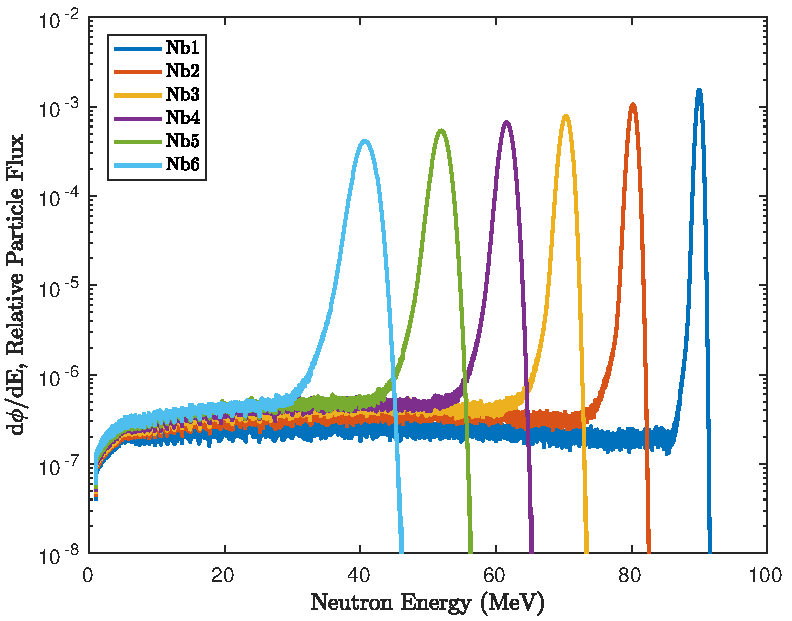
\includegraphics[width=0.5\linewidth]{./figures/Nb_ptallies.pdf}
 % Nb_ptallies.pdf: 380x298 pixel, 72dpi, 13.41x10.51 cm, bb=0 0 380 298
 \caption{Final variance minimized incident proton energy distributions for the Nb foils, as simulated in MCNP6. The distribution tallies in each foil are all normalized to be per source proton, which was $10^8$ in all simulations. As the beam is degraded, proton energy distributions become visibly broadened due to straggling, and drop in magnitude due to scattering losses.}
 \label{fig:Nb_ptallies}
\end{figure}

\begin{figure}
 \centering
 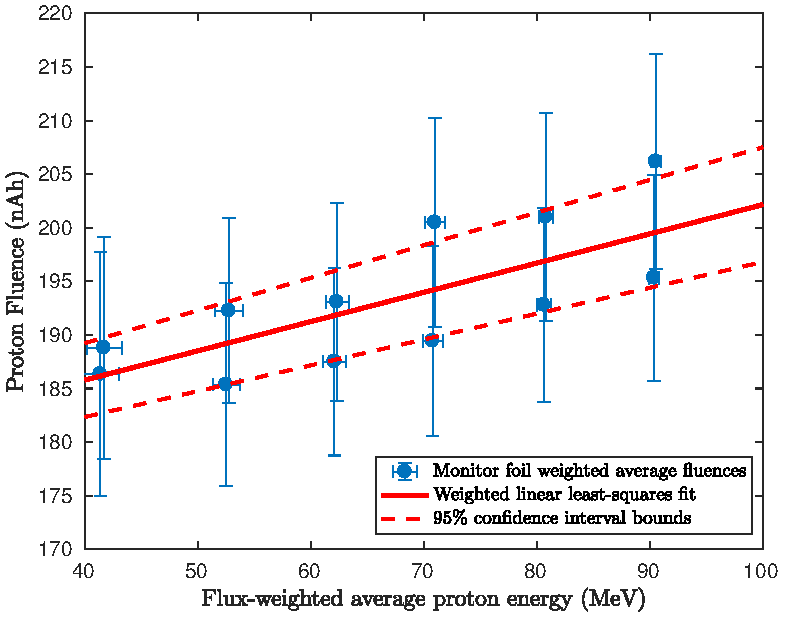
\includegraphics[width=0.5\linewidth]{./figures/fluence_plot.pdf}
 % Nb_ptallies.pdf: 380x298 pixel, 72dpi, 13.41x10.51 cm, bb=0 0 380 298
 \caption{Final uncertainty-weighted mean proton fluences throughout the target stack, based on the variance-minimized observed fluence from the the  \ce{^{nat}Cu}(p,x)\ce{^{56}Co}, \ce{^{nat}Cu}(p,x)\ce{^{62}Zn}, and \ce{^{nat}Cu}(p,x)\ce{^{65}Zn} monitor reactions. 
%  A 95\% ($2\sigma$) confidence interval is reported in the fitted proton fluence, to ensure a realistic uncertainty in fluence, which encompasses the true absolute fluence. 
  A clear loss of fluence  is visible, dropping by approximately 7.2--8.9\% from the incident fluence of 196.9--198.8 nAh over the length of the target stack, based on fluence loss models from MCNP6 simulations and an empirical fit to  fluence measurements.  This is due to a combination of beam utilization, as well as scattering.}
 \label{fig:fluence_plot}
\end{figure}







% \begin{equation}
% R = N_T \int_0^{E_{max}} \sigma(E) \dfrac{d\phi}{dE} dE
% \end{equation}





\subsection{Calculation of measured cross sections}\label{sec:calcs_sec}

%  include 1st and 2nd order bateman stuff here

Using the quantified EoB activities along with the variance-minimized proton fluence, it is possible to calculate the final cross sections for the various observed Nb(p,x) reactions.
While thin ($\approx$ 22 mg/cm$^2$) Nb foils were irradiated to minimize the energy width of these cross section measurements, it is important to note that all cross sections reported here are flux-averaged cross sections, over the energy distribution subtended by each foil, as seen in \autoref{fig:Nb_ptallies}.
For both the cumulative and independent activities quantified, cross sections were calculated as:
\begin{equation}
\sigma = \dfrac{A_0 }{\rho \Delta r I \pp{1-e^{-\lambda \Delta t}} }
\end{equation}
where $A_0$ is the EoB activity for the monitor reaction product, $I$ is the proton current, $\rho \Delta r$ is the foil's areal density, $\lambda$ is the monitor reaction product's decay constant, and $\Delta t$ is the length of irradiation.
The beam current, measured using an inductive pickup, remained stable for the duration of the irradiation, with the exception of approximately 70\,s of downtime,  occurring approximately 3 minutes into irradiation.
The propagated uncertainty in cross section is calculated as the quadrature sum of the uncertainty in quantified EoB activity (which includes uncertainty in detector efficiencies), uncertainty in the duration of irradiation (conservatively estimated at 60 s, to account for any transient changes in beam current), uncertainty in foil areal density, uncertainty in monitor product half-life (included, but normally negligible),  and uncertainty in proton current (quantified by error propagation of the monitor reaction fluence values  at each energy position, as seen in \autoref{fig:fluence_plot}).


% \begin{align}
% N_{\gamma} &= N_D \epsilon_\gamma I_\gamma \\
% &=  \epsilon_\gamma I_\gamma  \dfrac{N_T \sigma\pp{\bar{E}} \phi\pp{\bar{E}} }{\lambda}\pp{1 - e^{-\lambda t_i}}  e^{-\lambda t_d} \pp{1 - e^{-\lambda t_c}} \nonumber
% \end{align}



% \autoref{eqn:single_xs_eqn} can be used to determine the unknown (n,p) cross sections relative to the well-known \ce{^{115}In}(n,n')\ce{^{115m}In} and \ce{^{113}In}(n,n')\ce{^{113m}In} inelastic scattering cross sections since the Zn and Ti samples were co-irradiated with indium foils.
% This approach has a number of advantages since the result is independent of neutron flux and only depends on the relative detector efficiencies at each gamma-ray energy.
 

% \subsection{Systematic uncertainties}
% 
% XXXXXX




\section{Results}


After irradiation, all foils were confirmed to still be sealed inside their Kapton packets, verifying that no activation products were lost due to packet failure and dispersal.
In addition, each activated foil had a small \enquote{blister} under the Kapton tape layer, caused by a combination of thermal swelling and the formation of short-lived beta activities.
% \comment{Maybe some Ne formed by Al(p,2a)Ne / Si(p,2ap)Ne?}
This blister   shows the location where the primary proton beam was incident upon the foil.
The \ce{^{nat}Cu}(p,x)\ce{^{56}Co}, \ce{^{nat}Cu}(p,x)\ce{^{62}Zn}, and \ce{^{nat}Cu}(p,x)\ce{^{65}Zn} monitor reactions were used to determine the uncertainty-weighted mean fluence at each energy position (seen in \autoref{fig:fluence_plot}).
A fluence of 198.8$\pm$6.7 nAh was calculated to be incident upon the target stack using the MCNP6 fluence model, and a  fluence of 196.9$\pm$11.3 nAh using the linear fit model, both of which are consistent with the nominal fluence of 205.9 nAh based on IPF upstream current monitors.
As fluence loss in the target box's entrance window scales with $\sigma_{\mathrm{tot}}\rho\Delta r$, it is expected that an extrapolation back to the stack entrance will underestimate the nominal fluence incident upon the box.
This incident fluence dropped by approximately 8.9\% to  180.9$\pm$5.4 nAh (and by 7.2\% to  182.7$\pm$13.5 nAh using the linear fit model) over the length of the target stack, which is consistent with similar measurements at IPF in the past \cite{Graves2016}.
This loss of fluence is due to a combination of beam utilization for the various (p,x) reactions throughout the target stack, as well as large-angle deflections (primarily in the aluminum degraders) from scattering of the beam.





Using the final proton fluence at each energy position, cross sections for  \ce{^{51}Cr},  \ce{^{52g}Mn}, \ce{^{52m}Mn}, \ce{^{54}Mn}, \ce{^{55}Co}, \ce{^{56}Ni}, \ce{^{57}Ni}, \ce{^{57}Co},  \ce{^{58g}Co}, \ce{^{58m}Co}, \ce{^{59}Fe}, \ce{^{60}Co}, \ce{^{61}Cu}, and \ce{^{64}Cu} were extracted for (p,x) reactions  on \ce{^{nat}Cu} foils in the 40--90 MeV region, as recorded in \autoref{tab:cu_rp_table}.
For  (p,x) reactions on \ce{^{nat}Nb} foils, the (p,x) cross sections for \ce{^{82m}Rb}, \ce{^{83}Sr}, \ce{^{85g}Y}, \ce{^{85m}Y}, \ce{^{86}Zr}, \ce{^{86}Y}, \ce{^{87}Zr}, \ce{^{87g}Y}, \ce{^{87m}Y}, \ce{^{88}Zr}, \ce{^{88}Y}, \ce{^{89g}Nb}, \ce{^{89m}Nb}, \ce{^{89}Zr}, \ce{^{90}Mo}, \ce{^{90}Nb}, \ce{^{91m}Nb}, \ce{^{92m}Nb}, and \ce{^{93m}Mo} were extracted, as recorded in \autoref{tab:nb_rp_table}.
In addition, as there exist a number of isomers with radioactive ground states in these mass regions,  independent measurements of isomer-to-ground-state branching ratios for \ce{^{52m/g}Mn},\ce{^{58m/g}Co},\ce{^{85m/g}Y},\ce{^{87m/g}Y}, and \ce{^{89m/g}Nb} were  extracted and are recorded in \autoref{tab:ibr_table}.
Comparisons  of the measured cross sections and isomer branching ratios with literature data (retrieved from EXFOR \cite{Otuka2014272}) are seen in the figures of \ref{fit_figures} and \ref{ibr_figures}.
The propagated uncertainty in these cross sections varies widely based on the reaction product in question, with the major components  arising from uncertainty in EoB activity ($\pm$3--7\%), proton fluence ($\pm$4--6\%), and foil areal density ($\pm$0.1--0.6\%).
% \comment{Update these with new numbers!\\ Stephen: Very impressive, if you feel this is realistic. }




% % Please add the following required packages to your document preamble:
% % \usepackage{booktabs}
% \begin{table}
% \centering
% \caption{My caption}
% \label{my-label}
% \small
% \begin{tabular}{@{}lllllll@{}}
% \toprule
% E$_\text{p}$ (MeV) & $89.37^{+0.47}_{-0.45}$ & $79.55^{+0.68}_{-0.64}$ & $69.70^{+0.90}_{-0.85}$ & $61.07^{+1.05}_{-0.98}$ & $51.51^{+1.25}_{-1.21}$ & $40.34^{+1.58}_{-1.55}$ \\ \midrule
% 82mRb      & $2.39\pm0.18$           & --\cmmnt{\hrulefill}              & --\cmmnt{\hrulefill}              & --\cmmnt{\hrulefill}              & --\cmmnt{\hrulefill}              & --\cmmnt{\hrulefill}              \\
% 83Sr       & $3.88\pm0.56$           & $4.63\pm0.34$           & $3.42\pm0.32$           & --\cmmnt{\hrulefill}              & --\cmmnt{\hrulefill}              & --\cmmnt{\hrulefill}              \\
% 85cum Y    & $13.31\pm0.30$          & $7.28\pm0.44$           & $2.06\pm0.12$           & --\cmmnt{\hrulefill}              & --\cmmnt{\hrulefill}              & --\cmmnt{\hrulefill}              \\
% 85gY       & $2.286\pm0.057$         & $2.010\pm0.150$         & $0.545\pm0.030$         & --\cmmnt{\hrulefill}              & --\cmmnt{\hrulefill}              & --\cmmnt{\hrulefill}              \\
% 85mY       & $11.03\pm0.30$          & $5.27\pm0.42$           & $1.52\pm0.12$           & --\cmmnt{\hrulefill}              & --\cmmnt{\hrulefill}              & --\cmmnt{\hrulefill}              \\
% 86Zr       & $12.25\pm0.32$          & $17.63\pm0.44$          & $18.86\pm0.43$          & $6.00\pm0.15$           & --\cmmnt{\hrulefill}              & --\cmmnt{\hrulefill}              \\
% 86Y        & $32.25\pm0.89$          & $40.30\pm1.07$          & $39.02\pm1.00$          & $13.22\pm0.34$          & --\cmmnt{\hrulefill}              & --\cmmnt{\hrulefill}              \\
% 87Zr       & $45.82\pm5.82$          & $27.09\pm1.72$          & $31.46\pm1.49$          & $48.55\pm2.92$          & $37.66\pm1.58$          & $1.13\pm0.10$           \\
% 87cum Y    & $106.26\pm5.81$         & $52.92\pm1.70$          & $59.63\pm1.47$          & $87.77\pm2.90$          & $66.29\pm1.56$          & $2.93\pm0.10$           \\
% 87gY       & $27.03\pm5.45$          & $7.15\pm1.19$           & $6.41\pm0.55$           & $5.65\pm2.13$           & $2.59\pm0.45$           & $0.949\pm0.045$         \\
% 87mY       & $79.23\pm2.01$          & $45.78\pm1.22$          & $53.22\pm1.37$          & $82.12\pm1.97$          & $63.70\pm1.49$          & $1.98\pm0.09$           \\
% 88Zr       & $153.69\pm3.93$         & $140.02\pm3.48$         & $60.99\pm1.70$          & $20.65\pm0.49$          & $33.16\pm0.97$          & $65.82\pm1.32$          \\
% 88Y        & $16.64\pm0.76$          & $12.85\pm0.60$          & $7.81\pm0.61$           & $2.83\pm0.20$           & $9.05\pm1.33$           & $9.96\pm0.33$           \\
% 89cum Nb   & --\cmmnt{\hrulefill}              & --\cmmnt{\hrulefill}              & $175.52\pm12.44$        & $208.99\pm4.33$         & --\cmmnt{\hrulefill}              & --\cmmnt{\hrulefill}              \\
% 89gNb      & --\cmmnt{\hrulefill}              & --\cmmnt{\hrulefill}              & $141.58\pm12.28$        & $181.73\pm4.08$         & --\cmmnt{\hrulefill}              & --\cmmnt{\hrulefill}              \\
% 89mNb      & --\cmmnt{\hrulefill}              & --\cmmnt{\hrulefill}              & $33.94\pm1.97$          & $27.26\pm1.45$          & --\cmmnt{\hrulefill}              & --\cmmnt{\hrulefill}              \\
% 89Zr       & $203.76\pm5.32$         & $235.36\pm6.57$         & $287.50\pm6.76$         & $250.32\pm5.77$         & $54.63\pm1.15$          & $15.61\pm0.31$          \\
% 90Mo       & $20.57\pm0.68$          & $25.58\pm0.76$          & $33.75\pm0.90$          & $60.38\pm1.86$          & $120.28\pm2.93$         & $24.38\pm0.71$          \\
% 90Nb       & $152.93\pm4.72$         & $169.31\pm4.78$         & $204.70\pm5.79$         & $265.19\pm7.77$         & $363.35\pm9.78$         & $165.16\pm4.54$         \\
% 91mNb      & --\cmmnt{\hrulefill}              & --\cmmnt{\hrulefill}              & --\cmmnt{\hrulefill}              & --\cmmnt{\hrulefill}              & --\cmmnt{\hrulefill}              & $66.96\pm4.16$          \\
% 92mNb      & $42.18\pm1.15$          & $45.74\pm1.16$          & $48.75\pm1.21$          & $51.59\pm1.34$          & $54.49\pm1.37$          & $60.36\pm1.23$          \\
% 93mMo      & $0.93\pm0.18$           & $1.25\pm0.13$           & $1.58\pm0.22$           & $1.80\pm0.12$           & $1.83\pm0.10$           & $2.010\pm0.084$         \\ \bottomrule
% \end{tabular}
% \end{table}
% 
% % Please add the following required packages to your document preamble:
% % \usepackage{booktabs}
% \begin{table}[]
% \centering
% \caption{My caption}
% \label{my-label}
% \small
% \begin{tabular}{@{}llllllll@{}}
% \toprule
%       &            & \multicolumn{6}{c}{Production cross section (mb)}                                                                                                         \\ 
%       & E\_p (MeV) & $89.37^{+0.47}_{-0.45}$ & $79.55^{+0.68}_{-0.64}$ & $69.70^{+0.90}_{-0.85}$ & $61.07^{+1.05}_{-0.98}$ & $51.51^{+1.25}_{-1.21}$ & $40.34^{+1.58}_{-1.55}$ \\ \midrule
% 82mRb & $\sigma_c$ & $2.39\pm0.18$           & --\cmmnt{\hrulefill}              & --\cmmnt{\hrulefill}              & --\cmmnt{\hrulefill}              & --\cmmnt{\hrulefill}              & --\cmmnt{\hrulefill}              \\
% 83Sr  & $\sigma_c$ & $3.88\pm0.56$           & $4.63\pm0.34$           & $3.42\pm0.32$           & --\cmmnt{\hrulefill}              & --\cmmnt{\hrulefill}              & --\cmmnt{\hrulefill}              \\
% 85 Y  & $\sigma_c$ & $13.31\pm0.30$          & $7.28\pm0.44$           & $2.06\pm0.12$           & --\cmmnt{\hrulefill}              & --\cmmnt{\hrulefill}              & --\cmmnt{\hrulefill}              \\
% 85gY  & $\sigma_i$ & $2.286\pm0.057$         & $2.010\pm0.150$         & $0.545\pm0.030$         & --\cmmnt{\hrulefill}              & --\cmmnt{\hrulefill}              & --\cmmnt{\hrulefill}              \\
% 85mY  & $\sigma_i$ & $11.03\pm0.30$          & $5.27\pm0.42$           & $1.52\pm0.12$           & --\cmmnt{\hrulefill}              & --\cmmnt{\hrulefill}              & --\cmmnt{\hrulefill}              \\
% 86Zr  & $\sigma_c$ & $12.25\pm0.32$          & $17.63\pm0.44$          & $18.86\pm0.43$          & $6.00\pm0.15$           & --\cmmnt{\hrulefill}              & --\cmmnt{\hrulefill}              \\
% 86Y   & $\sigma_c$ & $32.25\pm0.89$          & $40.30\pm1.07$          & $39.02\pm1.00$          & $13.22\pm0.34$          & --\cmmnt{\hrulefill}              & --\cmmnt{\hrulefill}              \\
% 87Zr  & $\sigma_c$ & $45.82\pm5.82$          & $27.09\pm1.72$          & $31.46\pm1.49$          & $48.55\pm2.92$          & $37.66\pm1.58$          & $1.13\pm0.10$           \\
% 87 Y  & $\sigma_c$ & $106.26\pm5.81$         & $52.92\pm1.70$          & $59.63\pm1.47$          & $87.77\pm2.90$          & $66.29\pm1.56$          & $2.93\pm0.10$           \\
% 87gY  & $\sigma_i$ & $27.03\pm5.45$          & $7.15\pm1.19$           & $6.41\pm0.55$           & $5.65\pm2.13$           & $2.59\pm0.45$           & $0.949\pm0.045$         \\
% 87mY  & $\sigma_i$ & $79.23\pm2.01$          & $45.78\pm1.22$          & $53.22\pm1.37$          & $82.12\pm1.97$          & $63.70\pm1.49$          & $1.98\pm0.09$           \\
% 88Zr  & $\sigma_c$ & $153.69\pm3.93$         & $140.02\pm3.48$         & $60.99\pm1.70$          & $20.65\pm0.49$          & $33.16\pm0.97$          & $65.82\pm1.32$          \\
% 88Y   & $\sigma_c$ & $16.64\pm0.76$          & $12.85\pm0.60$          & $7.81\pm0.61$           & $2.83\pm0.20$           & $9.05\pm1.33$           & $9.96\pm0.33$           \\
% 89 Nb & $\sigma_c$ & --\cmmnt{\hrulefill}              & --\cmmnt{\hrulefill}              & $175.52\pm12.44$        & $208.99\pm4.33$         & --\cmmnt{\hrulefill}              & --\cmmnt{\hrulefill}              \\
% 89gNb & $\sigma_i$ & --\cmmnt{\hrulefill}              & --\cmmnt{\hrulefill}              & $141.58\pm12.28$        & $181.73\pm4.08$         & --\cmmnt{\hrulefill}              & --\cmmnt{\hrulefill}              \\
% 89mNb & $\sigma_i$ & --\cmmnt{\hrulefill}              & --\cmmnt{\hrulefill}              & $33.94\pm1.97$          & $27.26\pm1.45$          & --\cmmnt{\hrulefill}              & --\cmmnt{\hrulefill}              \\
% 89Zr  & $\sigma_c$ & $203.76\pm5.32$         & $235.36\pm6.57$         & $287.50\pm6.76$         & $250.32\pm5.77$         & $54.63\pm1.15$          & $15.61\pm0.31$          \\
% 90Mo  & $\sigma_c$ & $20.57\pm0.68$          & $25.58\pm0.76$          & $33.75\pm0.90$          & $60.38\pm1.86$          & $120.28\pm2.93$         & $24.38\pm0.71$          \\
% 90Nb  & $\sigma_c$ & $152.93\pm4.72$         & $169.31\pm4.78$         & $204.70\pm5.79$         & $265.19\pm7.77$         & $363.35\pm9.78$         & $165.16\pm4.54$         \\
% 91mNb & $\sigma_c$ & --\cmmnt{\hrulefill}              & --\cmmnt{\hrulefill}              & --\cmmnt{\hrulefill}              & --\cmmnt{\hrulefill}              & --\cmmnt{\hrulefill}              & $66.96\pm4.16$          \\
% 92mNb & $\sigma_c$ & $42.18\pm1.15$          & $45.74\pm1.16$          & $48.75\pm1.21$          & $51.59\pm1.34$          & $54.49\pm1.37$          & $60.36\pm1.23$          \\
% 93mMo & $\sigma_c$ & $0.93\pm0.18$           & $1.25\pm0.13$           & $1.58\pm0.22$           & $1.80\pm0.12$           & $1.83\pm0.10$           & $2.010\pm0.084$         \\ \bottomrule
% \end{tabular}
% \end{table}
% 
% % Please add the following required packages to your document preamble:
% % \usepackage{booktabs}
% \begin{table}[]
% \centering
% \caption{My caption}
% \label{my-label}
% \small
% \begin{tabular}{@{}llllllll@{}}
% \toprule
%       &            & \multicolumn{6}{c}{Production cross section (mb)}                                                                                                         \\ \cmidrule(l){3-8} 
%       & E\_p (MeV) & $89.37^{+0.47}_{-0.45}$ & $79.55^{+0.68}_{-0.64}$ & $69.70^{+0.90}_{-0.85}$ & $61.07^{+1.05}_{-0.98}$ & $51.51^{+1.25}_{-1.21}$ & $40.34^{+1.58}_{-1.55}$ \\ \midrule
% \ce{^{82m}Rb} & $\sigma_c$ & $2.39\pm0.18$           & --\cmmnt{\hrulefill}              & --\cmmnt{\hrulefill}              & --\cmmnt{\hrulefill}              & --\cmmnt{\hrulefill}              & --\cmmnt{\hrulefill}              \\
% 83Sr  & $\sigma_c$ & $3.88\pm0.56$           & $4.63\pm0.34$           & $3.42\pm0.32$           & --\cmmnt{\hrulefill}              & --\cmmnt{\hrulefill}              & --\cmmnt{\hrulefill}              \\
% 85 Y  & $\sigma_c$ & $13.31\pm0.30$          & $7.28\pm0.44$           & $2.06\pm0.12$           & --\cmmnt{\hrulefill}              & --\cmmnt{\hrulefill}              & --\cmmnt{\hrulefill}              \\
% 85gY  & $\sigma_i$ & $2.286\pm0.057$         & $2.010\pm0.150$         & $0.545\pm0.030$         & --\cmmnt{\hrulefill}              & --\cmmnt{\hrulefill}              & --\cmmnt{\hrulefill}              \\
% 85mY  & $\sigma_i$ & $11.03\pm0.30$          & $5.27\pm0.42$           & $1.52\pm0.12$           & --\cmmnt{\hrulefill}              & --\cmmnt{\hrulefill}              & --\cmmnt{\hrulefill}              \\
% 86Zr  & $\sigma_c$ & $12.25\pm0.32$          & $17.63\pm0.44$          & $18.86\pm0.43$          & $6.00\pm0.15$           & --\cmmnt{\hrulefill}              & --\cmmnt{\hrulefill}              \\
% 86Y   & $\sigma_c$ & $32.25\pm0.89$          & $40.30\pm1.07$          & $39.02\pm1.00$          & $13.22\pm0.34$          & --\cmmnt{\hrulefill}              & --\cmmnt{\hrulefill}              \\
% 87Zr  & $\sigma_c$ & $45.82\pm5.82$          & $27.09\pm1.72$          & $31.46\pm1.49$          & $48.55\pm2.92$          & $37.66\pm1.58$          & $1.13\pm0.10$           \\
% 87 Y  & $\sigma_c$ & $106.26\pm5.81$         & $52.92\pm1.70$          & $59.63\pm1.47$          & $87.77\pm2.90$          & $66.29\pm1.56$          & $2.93\pm0.10$           \\
% 87gY  & $\sigma_i$ & $27.03\pm5.45$          & $7.15\pm1.19$           & $6.41\pm0.55$           & $5.65\pm2.13$           & $2.59\pm0.45$           & $0.949\pm0.045$         \\
% 87mY  & $\sigma_i$ & $79.23\pm2.01$          & $45.78\pm1.22$          & $53.22\pm1.37$          & $82.12\pm1.97$          & $63.70\pm1.49$          & $1.98\pm0.09$           \\
% 88Zr  & $\sigma_c$ & $153.69\pm3.93$         & $140.02\pm3.48$         & $60.99\pm1.70$          & $20.65\pm0.49$          & $33.16\pm0.97$          & $65.82\pm1.32$          \\
% 88Y   & $\sigma_c$ & $16.64\pm0.76$          & $12.85\pm0.60$          & $7.81\pm0.61$           & $2.83\pm0.20$           & $9.05\pm1.33$           & $9.96\pm0.33$           \\
% 89 Nb & $\sigma_c$ & --\cmmnt{\hrulefill}              & --\cmmnt{\hrulefill}              & $175.52\pm12.44$        & $208.99\pm4.33$         & --\cmmnt{\hrulefill}              & --\cmmnt{\hrulefill}              \\
% 89gNb & $\sigma_i$ & --\cmmnt{\hrulefill}              & --\cmmnt{\hrulefill}              & $141.58\pm12.28$        & $181.73\pm4.08$         & --\cmmnt{\hrulefill}              & --\cmmnt{\hrulefill}              \\
% 89mNb & $\sigma_i$ & --\cmmnt{\hrulefill}              & --\cmmnt{\hrulefill}              & $33.94\pm1.97$          & $27.26\pm1.45$          & --\cmmnt{\hrulefill}              & --\cmmnt{\hrulefill}              \\
% 89Zr  & $\sigma_c$ & $203.76\pm5.32$         & $235.36\pm6.57$         & $287.50\pm6.76$         & $250.32\pm5.77$         & $54.63\pm1.15$          & $15.61\pm0.31$          \\
% 90Mo  & $\sigma_c$ & $20.57\pm0.68$          & $25.58\pm0.76$          & $33.75\pm0.90$          & $60.38\pm1.86$          & $120.28\pm2.93$         & $24.38\pm0.71$          \\
% 90Nb  & $\sigma_c$ & $152.93\pm4.72$         & $169.31\pm4.78$         & $204.70\pm5.79$         & $265.19\pm7.77$         & $363.35\pm9.78$         & $165.16\pm4.54$         \\
% 91mNb & $\sigma_c$ & --\cmmnt{\hrulefill}              & --\cmmnt{\hrulefill}              & --\cmmnt{\hrulefill}              & --\cmmnt{\hrulefill}              & --\cmmnt{\hrulefill}              & $66.96\pm4.16$          \\
% 92mNb & $\sigma_c$ & $42.18\pm1.15$          & $45.74\pm1.16$          & $48.75\pm1.21$          & $51.59\pm1.34$          & $54.49\pm1.37$          & $60.36\pm1.23$          \\
% 93mMo & $\sigma_c$ & $0.93\pm0.18$           & $1.25\pm0.13$           & $1.58\pm0.22$           & $1.80\pm0.12$           & $1.83\pm0.10$           & $2.010\pm0.084$         \\ \bottomrule
% \end{tabular}
% \end{table}



% Please add the following required packages to your document preamble:
% \usepackage{booktabs}
\begin{table}
\centering
\caption{Measured cross sections for the various \ce{^{nat}Cu}(p,x) reaction products observed in this work. Cumulative cross sections are designated as $\sigma_c$, independent cross sections are designated as $\sigma_i$.}
\label{tab:cu_rp_table}
\small
\resizebox{\textwidth}{!}{%
\begin{tabular}{@{}lllllll@{}}
\toprule
                            & \multicolumn{6}{c}{Production cross section (mb)}                                                                                                         \\ \cmidrule(l){2-7} 
E$_\text{p}$ (MeV)          & $89.74^{+0.48}_{-0.43}$ & $79.95^{+0.67}_{-0.64}$ & $70.17^{+0.91}_{-0.85}$ & $61.58^{+1.03}_{-0.98}$ & $52.10^{+1.25}_{-1.20}$ & $41.05^{+1.62}_{-1.54}$ \\ \midrule
\ce{^{51}Cr}\,($\sigma_c$)  & $0.919\pm0.079$         & $0.373\pm0.023$         & $0.450\pm0.028$         & $0.303\pm0.016$         & --\cmmnt{\hrulefill}    & --\cmmnt{\hrulefill}    \\
\ce{^{52}Mn}\,($\sigma_c$)  & $1.70\pm0.11$           & $0.570\pm0.031$         & $0.0407\pm0.0022$       & $0.00526\pm0.00057$     & --\cmmnt{\hrulefill}    & --\cmmnt{\hrulefill}    \\
\ce{^{52g}Mn}\,($\sigma_i$) & $0.673\pm0.043$         & $0.239\pm0.018$         & $0.0164\pm0.0023$       & $0.000986\pm0.000053$   & --\cmmnt{\hrulefill}    & --\cmmnt{\hrulefill}    \\
\ce{^{52m}Mn}\,($\sigma_c$) & $1.023\pm0.091$         & $0.331\pm0.030$         & $0.0244\pm0.0036$       & $0.00427\pm0.00052$     & --\cmmnt{\hrulefill}    & --\cmmnt{\hrulefill}    \\
\ce{^{54}Mn}\,($\sigma_i$)  & $5.87\pm0.37$           & $3.77\pm0.21$           & $4.14\pm0.22$           & $4.84\pm0.26$           & $1.680\pm0.091$         & --\cmmnt{\hrulefill}    \\
\ce{^{55}Co}\,($\sigma_c$)  & $1.71\pm0.11$           & $1.015\pm0.058$         & $0.193\pm0.012$         & $0.0299\pm0.0028$       & $0.00235\pm0.00022$     & --\cmmnt{\hrulefill}    \\
\ce{^{56}Ni}\,($\sigma_c$)  & $0.0806\pm0.0051$       & $0.1005\pm0.0055$       & $0.0906\pm0.0046$       & $0.0304\pm0.0016$       & --\cmmnt{\hrulefill}    & --\cmmnt{\hrulefill}    \\
\ce{^{57}Ni}\,($\sigma_c$)  & $1.465\pm0.093$         & $1.202\pm0.065$         & $1.400\pm0.071$         & $2.13\pm0.11$           & $1.565\pm0.083$         & $0.0262\pm0.0015$       \\
\ce{^{57}Co}\,($\sigma_i$)  & $40.1\pm2.5$          & $35.6\pm1.9$          & $35.8\pm1.8$          & $48.5\pm2.5$            & $47.7\pm2.5$            & $3.21\pm0.18$           \\
\ce{^{58}Co}\,($\sigma_c$)  & $57.7\pm4.5$            & $55.0\pm4.7$            & $42.7\pm3.4$            & $33.7\pm2.8$            & $39.0\pm3.8$            & $62.3\pm4.6$            \\
\ce{^{58g}Co}\,($\sigma_i$) & $14.0\pm2.5$            & $10.8\pm2.1$            & $6.1\pm1.6$             & $7.8\pm1.4$             & $7.1\pm1.7$             & $1.12\pm0.32$           \\
\ce{^{58m}Co}\,($\sigma_i$) & $43.6\pm3.7$            & $44.2\pm4.3$            & $36.6\pm3.0$            & $25.8\pm2.5$            & $31.9\pm3.3$            & $61.1\pm4.6$            \\
\ce{^{59}Fe}\,($\sigma_c$)  & $0.865\pm0.057$         & $0.837\pm0.046$         & $0.749\pm0.039$         & $0.616\pm0.034$         & $0.209\pm0.014$         & --\cmmnt{\hrulefill}    \\
\ce{^{60}Co}\,($\sigma_c$)  & $13.23\pm0.87$          & $13.47\pm0.78$          & $11.14\pm0.94$          & $11.44\pm0.80$          & $9.30\pm0.87$           & $6.6\pm1.1$             \\
\ce{^{61}Cu}\,($\sigma_c$)  & $50.5\pm3.3$            & $56.1\pm3.2$            & $65.1\pm3.6$            & $72.2\pm4.0$            & $80.6\pm4.7$            & $157.1\pm8.6$           \\
\ce{^{64}Cu}\,($\sigma_i$)  & $38.7\pm2.7$            & $42.8\pm2.4$            & $45.5\pm2.7$            & $50.2\pm2.8$            & $55.7\pm3.0$            & $63.3\pm3.6$                 \\ \bottomrule
\end{tabular}
}
\end{table}

% Please add the following required packages to your document preamble:
% \usepackage{booktabs}
\begin{table}
\centering
\caption{Measured cross sections for the various \ce{^{nat}Nb}(p,x) reaction products observed in this work. Cumulative cross sections are designated as $\sigma_c$, independent cross sections are designated as $\sigma_i$.}
\label{tab:nb_rp_table}
\small
\begin{tabular}{@{}lllllll@{}}
\toprule
                            & \multicolumn{6}{c}{Production cross section (mb)}                                                                                                         \\ \cmidrule(l){2-7} 
E$_\text{p}$ (MeV)          & $89.37^{+0.47}_{-0.45}$ & $79.55^{+0.68}_{-0.64}$ & $69.70^{+0.90}_{-0.85}$ & $61.07^{+1.05}_{-0.98}$ & $51.51^{+1.25}_{-1.21}$ & $40.34^{+1.58}_{-1.55}$ \\ \midrule
\ce{^{82m}Rb}\,($\sigma_c$) & $2.48\pm0.22$           & --\cmmnt{\hrulefill}    & --\cmmnt{\hrulefill}    & --\cmmnt{\hrulefill}    & --\cmmnt{\hrulefill}    & --\cmmnt{\hrulefill}    \\
\ce{^{83}Sr}\,($\sigma_c$)  & $4.02\pm0.61$           & $4.78\pm0.42$           & $3.49\pm0.36$           & --\cmmnt{\hrulefill}    & --\cmmnt{\hrulefill}    & --\cmmnt{\hrulefill}    \\
\ce{^{85}Y}\,($\sigma_c$)   & $13.78\pm0.55$          & $7.52\pm0.51$           & $2.11\pm0.14$           & --\cmmnt{\hrulefill}    & --\cmmnt{\hrulefill}    & --\cmmnt{\hrulefill}    \\
\ce{^{85g}Y}\,($\sigma_i$)  & $2.37\pm0.11$           & $2.08\pm0.17$           & $0.557\pm0.037$         & --\cmmnt{\hrulefill}    & --\cmmnt{\hrulefill}    & --\cmmnt{\hrulefill}    \\
\ce{^{85m}Y}\,($\sigma_i$)  & $11.41\pm0.54$          & $5.44\pm0.48$           & $1.55\pm0.13$           & --\cmmnt{\hrulefill}    & --\cmmnt{\hrulefill}    & --\cmmnt{\hrulefill}    \\
\ce{^{86}Zr}\,($\sigma_c$)  & $12.68\pm0.68$          & $18.21\pm0.93$          & $19.28\pm0.97$          & $6.16\pm0.32$           & --\cmmnt{\hrulefill}    & --\cmmnt{\hrulefill}    \\
\ce{^{86}Y}\,($\sigma_i$)   & $33.4\pm1.8$            & $41.6\pm2.2$            & $39.9\pm2.1$            & $13.56\pm0.72$          & --\cmmnt{\hrulefill}    & --\cmmnt{\hrulefill}    \\
\ce{^{87}Zr}\,($\sigma_c$)  & $47.4\pm7.3$            & $28.0\pm2.8$            & $32.2\pm2.9$            & $49.8\pm5.0$            & $38.2\pm3.7$            & $1.12\pm0.17$           \\
\ce{^{87}Y}\,($\sigma_i$)   & $110.0\pm7.2$           & $54.7\pm2.8$            & $61.0\pm2.9$            & $90.0\pm4.9$            & $67.2\pm3.6$            & $2.91\pm0.17$           \\
\ce{^{87g}Y}\,($\sigma_i$)  & $28.0\pm5.8$            & $7.4\pm1.3$             & $6.55\pm0.64$           & $5.8\pm2.2$             & $2.63\pm0.47$           & $0.942\pm0.073$         \\
\ce{^{87m}Y}\,($\sigma_i$)  & $82.0\pm4.3$            & $47.3\pm2.5$            & $54.4\pm2.8$            & $84.2\pm4.4$            & $64.6\pm3.6$            & $1.97\pm0.15$           \\
\ce{^{88}Zr}\,($\sigma_c$)  & $159.1\pm7.8$           & $144.6\pm6.8$           & $62.4\pm3.1$            & $21.2\pm1.0$            & $33.6\pm1.8$            & $65.3\pm4.0$            \\
\ce{^{88}Y}\,($\sigma_i$)   & $17.2\pm1.1$            & $13.27\pm0.86$          & $7.98\pm0.72$           & $2.91\pm0.25$           & $9.2\pm1.4$             & $9.88\pm0.69$           \\
\ce{^{89}Nb}\,($\sigma_c$)  & --\cmmnt{\hrulefill}    & --\cmmnt{\hrulefill}    & $179\pm14$              & $214.4\pm9.8$           & --\cmmnt{\hrulefill}    & --\cmmnt{\hrulefill}    \\
\ce{^{89g}Nb}\,($\sigma_i$) & --\cmmnt{\hrulefill}    & --\cmmnt{\hrulefill}    & $145\pm14$              & $186.4\pm9.6$           & --\cmmnt{\hrulefill}    & --\cmmnt{\hrulefill}    \\
\ce{^{89m}Nb}\,($\sigma_i$) & --\cmmnt{\hrulefill}    & --\cmmnt{\hrulefill}    & $34.7\pm2.6$            & $28.0\pm2.0$            & --\cmmnt{\hrulefill}    & --\cmmnt{\hrulefill}    \\
\ce{^{89}Zr}\,($\sigma_i$)  & $211\pm11$              & $243\pm13$              & $294\pm15$              & $257\pm13$              & $55.4\pm3.0$            & $15.5\pm1.0$            \\
\ce{^{90}Mo}\,($\sigma_i$)  & $21.3\pm1.1$            & $26.4\pm1.3$            & $34.5\pm1.6$            & $61.9\pm3.1$            & $122.0\pm6.1$           & $24.2\pm1.5$            \\
\ce{^{90}Nb}\,($\sigma_i$)  & $158.3\pm8.1$           & $174.9\pm8.5$           & $209.3\pm9.9$           & $272\pm14$              & $369\pm19$              & $163.9\pm9.8$           \\
\ce{^{91m}Nb}\,($\sigma_c$) & --\cmmnt{\hrulefill}    & --\cmmnt{\hrulefill}    & --\cmmnt{\hrulefill}    & --\cmmnt{\hrulefill}    & --\cmmnt{\hrulefill}    & $66.5\pm5.8$            \\
\ce{^{92m}Nb}\,($\sigma_i$) & $43.7\pm2.4$            & $47.3\pm2.4$            & $49.8\pm2.6$            & $52.9\pm2.8$            & $55.3\pm3.1$            & $59.9\pm3.9$            \\
\ce{^{93m}Mo}\,($\sigma_i$) & $0.97\pm0.20$           & $1.29\pm0.15$           & $1.62\pm0.24$           & $1.85\pm0.15$           & $1.86\pm0.14$           & $2.00\pm0.15$               \\ \bottomrule
\end{tabular}
\end{table}






% Please add the following required packages to your document preamble:
% \usepackage{booktabs}
\begin{table}
\centering
\caption{Measured isomer-to-ground-state branching ratios for the various \ce{^{nat}Nb}(p,x) and \ce{^{nat}Cu}(p,x) reaction products observed in this work.}
\label{tab:ibr_table}
\small
\resizebox{\textwidth}{!}{%
\begin{tabular}{@{}lllllll@{}}
\toprule
                               & \multicolumn{6}{c}{Isomer branching ratio}                                                                                                                \\ \cmidrule(l){2-7} 
E$_\text{p}$ (MeV)             & $89.74^{+0.48}_{-0.43}$ & $79.95^{+0.67}_{-0.64}$ & $70.17^{+0.91}_{-0.85}$ & $61.58^{+1.03}_{-0.98}$ & $52.10^{+1.25}_{-1.20}$ & $41.05^{+1.62}_{-1.54}$ \\ \midrule
\ce{^{nat}Cu}(p,x)\ce{^{52}Mn} & $0.603\pm0.066$         & $0.581\pm0.062$         & $0.598\pm0.095$         & $0.81\pm0.13$           & --\cmmnt{\hrulefill}    & --\cmmnt{\hrulefill}    \\
\ce{^{nat}Cu}(p,x)\ce{^{58}Co} & $0.757\pm0.088$         & $0.80\pm0.10$         & $0.858\pm0.099$         & $0.767\pm0.097$         & $0.82\pm0.12$           & $0.98\pm0.10$            \vspace{1em}     \\ 
E$_\text{p}$ (MeV)             & $89.37^{+0.47}_{-0.45}$ & $79.55^{+0.68}_{-0.64}$ & $69.70^{+0.90}_{-0.85}$ & $61.07^{+1.05}_{-0.98}$ & $51.51^{+1.25}_{-1.21}$ & $40.34^{+1.58}_{-1.55}$ \\ \midrule
\ce{^{nat}Nb}(p,x)\ce{^{85}Y}  & $0.828\pm0.051$         & $0.724\pm0.080$         & $0.736\pm0.080$         & --\cmmnt{\hrulefill}    & --\cmmnt{\hrulefill}    & --\cmmnt{\hrulefill}    \\
\ce{^{nat}Nb}(p,x)\ce{^{87}Y}  & $0.746\pm0.063$         & $0.865\pm0.063$         & $0.893\pm0.063$         & $0.936\pm0.070$         & $0.961\pm0.075$         & $0.676\pm0.065$         \\
\ce{^{nat}Nb}(p,x)\ce{^{89}Nb} & --\cmmnt{\hrulefill}    & --\cmmnt{\hrulefill}    & $0.193\pm0.021$         & $0.130\pm0.011$         & --\cmmnt{\hrulefill}    & --\cmmnt{\hrulefill}    \\ \bottomrule
\end{tabular}
}
\end{table}





These results have several notable takeaways.
The various \ce{^{nat}Cu}(p,x) cross sections measured here are in excellent agreement with the body of measurements in the literature,  but have been measured nearly exclusively with the highest precision to date.
Similarly, the various \ce{^{nat}Nb}(p,x) cross sections measured here are in excellent agreement with literature data, which is far more sparse in the 40--90 MeV region than for \ce{^{nat}Cu}(p,x) ---  less than 3 existing measurements have been performed for the majority of the reactions presented here.
Indeed,  the \ce{^{nat}Nb}(p,x)\ce{^{83}Sr}, \ce{^{nat}Nb}(p,x)\ce{^{85}Y}, \ce{^{nat}Nb}(p,x)\ce{^{89}Nb}, \ce{^{nat}Nb}(p,x)\ce{^{90}Mo}, \ce{^{nat}Nb}(p,x)\ce{^{91m}Nb}, and \ce{^{nat}Nb}(p,x)\ce{^{98m}Mo} reactions each possess no more than a total of 3 data points in this energy region.
Not only do the \ce{^{nat}Nb}(p,x) measurements in this work fill in the sparse data in this energy region, but they have been measured with the highest precision relative to existing literature data.



Furthermore, this work presents the first measurements of several observables in these mass regions.
This work reports the first experimental measurement of the \ce{^{nat}Nb}(p,x)\ce{^{82m}Rb} reaction in the 40--90 MeV region.
It also represents  the first measurement of the independent cross section for       \ce{^{nat}Cu}(p,x)\ce{^{52\text{g}}Mn}, as well as the \ce{^{52\text{m}}Mn} ($2^+$) / \ce{^{52\text{g}}Mn}  ($6^+$)  isomer branching ratio via \ce{^{nat}Cu}(p,x).  
The cumulative cross sections from these data are also consistent with existing measurements of the cumulative \ce{^{nat}Cu}(p,x)\ce{^{52}Mn} cross section.
Similarly, this work offers the first measurement of the independent cross sections for \ce{^{nat}Nb}(p,x)\ce{^{85\text{g}}Y},  as well as the first measurement of the     \ce{^{85\text{m}}Y} ($\sfrac{9}{2}^+$) / \ce{^{85\text{g}}Y}  ($\sfrac{1}{2}^-$) isomer branching ratio via \ce{^{nat}Nb}(p,x).



Notably, this work serves as the most well-characterized measurement of the \ce{^{nat}Nb}(p,x)\ce{^{90}Mo} reaction below 100 MeV to date, with cross sections measured  at the 4--6\% uncertainty level.
This is important, as it presents the first step towards characterizing this reaction for use as a proton monitor reaction standard below 100 MeV.
The quantification of \ce{^{90}Mo} activity proved to be one of the most straightforward of all reaction products observed in this work.
\ce{^{nat}Nb}(p,x)\ce{^{90}Mo} can only be populated through the (p,4n) reaction channel, so no corrections for (n,x) contamination channels or decay down the A=90 isobar are needed, which makes activity quantification trivial.
In addition, \ce{^{90}Mo}  possesses seven strong, distinct gamma lines which can easily  be used for its identification and quantification.
Finally, the production of \ce{^{90}Mo}  in the 40--90 MeV region is quite strong, with a peak cross section of approximately 120 mb.
Combining the reaction yield and gamma abundance, the use of approximately 23 mg/cm$^2$ Nb targets easily provided sufficient counting statistics for activity quantification in the 40--90 MeV region.
This result presents the first step towards the use of \ce{^{90}Mo} as a clean and precise   charged particle monitor reaction standard in irradiations up to approximately 24 hours in duration.





In addition to the $^\text{nat}$Nb(p,x)\ce{^{90}Mo} measurement, this experiment has also yielded measurements of  a number of additional  emerging radionuclides with medical applications.
These include the non-standard positron emitters \ce{^{57}Ni},  \ce{^{86}Y}, \ce{^{89}Zr},  \ce{^{90}Nb}, the $\beta^-$-therapy agent  \ce{^{64}Cu},  and the Auger-therapy agent \ce{^{82\text{m}}Rb}. 



\ce{^{57}Ni} ($t_{1/2}=35.60\pm0.06$ h, $\epsilon$=100\% to \ce{^{57}Co} \cite{Bhat1998}), while useful on its own as a positron emitter, stands poised as a particularly promising candidate for theranostic pairing with the soft $\beta^-$ emitter \ce{^{66}Ni} ($t_{1/2}=54.6\pm0.3$ h, $\beta^-$=100\% to \ce{^{66}Cu} \cite{Browne2010a}) \cite{PMID:7632762,zweit1996medium,Graves2016,Rosch2014}. 
\ce{^{nat}Cu}(p,x)\ce{^{57}Ni} would seem to be an intriguing production pathway, due to the ready availability of Cu metal as target, combined with the fact that production in this pathway strongly favors \ce{^{57}Ni} over \ce{^{56}Ni} --- indeed, the \ce{^{57}Ni}/\ce{^{56}Ni} 
%ratio of cross sections is approximately 70 at 61.58 MeV, and varies from 11-18 at the 70-90 MeV positions.
ratio of production rates is approximately 290 at 61.58 MeV, and varies from 45--75 at the 70--90 MeV positions.
The traditional route for \ce{^{57}Ni} production is via \ce{^{nat}Co}(p,3n)\ce{^{57}Ni}, but at moderate energies, suffers from more  \ce{^{56}Ni} contamination than \ce{^{nat}Cu}(p,x)  ($\sigma_\text{57Ni} / \sigma_\text{56Ni}\approx$ 10 at maximum).
Lower-energy production via \ce{^{nat}Co}(p,3n) at 24--40 MeV is below threshold for \ce{^{56}Ni}, but has a peak cross section of approximately 10 mb, making \ce{^{nat}Cu}(p,x) the superior production route for moderate-energy accelerators  \cite{MICHEL1997153,Ditrói2013}.


\ce{^{86}Y} ($t_{1/2}=14.74\pm0.02$ h, $\epsilon$=100\% to \ce{^{86}Sr}  \cite{NEGRET20151}) is another novel  emerging  PET isotope, whose longer half-life has poised it for applications as a tracer for slower metabolic processes, as well as in   pharmacokinetics studies \cite{Valdovinos2017,Nickles2003,Qaim2008,QaimSyedM2011}.
In particular, it is highly desired to form a theranostic pair with the widely-employed $\beta^-$ therapy agent \ce{^{90}Y} ($t_{1/2}=64.00\pm0.21$ h, $\beta^-$=100\% to \ce{^{90}Zr} \cite{Browne1997}), which can be produced from a long-lived \ce{^{90}Sr} cow and emits no discrete observable gamma-rays or x-rays though decay \cite{Herzog1993}.
Although a weak positron branch exists and bremsstrahlung scintigraphy is commonly used for clinical imaging of the \ce{^{90}Y} biodistribution, theranostics  necessitate an imaging isotope to be paired for quantification of its uptake and biodistribution  \cite{Nickles2004}.
Conventional production of \ce{^{86}Y} proceeds through low-energy (7--14 MeV) irradiation via \ce{^{86}Sr}(p,n), which requires an enriched  \ce{^{86}Sr} target (9.86\% natural abundance), in order to eliminate contamination from (p,n) on the other stable \ce{^{84,87,88}Sr} isotopes  \cite{Rosch1993}.
Alternatively, production at 33--43 MeV via \ce{^{88}Sr}(p,3n) has been proposed --- this pathway also requires an enriched target (82.58\% natural abundance) for the same reason, but contamination with other Y co-activities will be even more pronounced than via (p,n), due to the opening of (p,n) and (p,2n) channels on all stable Sr isotopes \cite{doi:10.1139/v67-193,levkovski1991cross}.
Minimizing activity from other isotopes of the element in question is essential for producing radionuclides in high specific activity, as these competing isotopes are often impractical to separate out by radiochemical means.
% \comment{Stephen:  impossible by radiochemical means, and impossible by affordable/practical means.\\Substitute for ``difficult'' post-discussion.}
As a result, it would appear that \ce{^{nat}Nb}(p,x) is a poor route for  \ce{^{86}Y} production in this respect, as it only reaches a maximum of approximately 35\% radioisotopic purity.
The  dominant yttrium radioisotope produced by  \ce{^{nat}Nb}(p,x) in the 40--90 MeV region is  \ce{^{87}Y} ($t_{1/2}=79.8\pm0.3$ h, $\epsilon^-$=100\% to \ce{^{87m}Sr} \cite{Johnson2015}).
However,  \ce{^{87}Y} itself has application as a generator for  \ce{^{87m}Sr} ($t_{1/2}=2.815\pm0.012$ h, IT=99.70\% to \ce{^{87}Sr} \cite{Johnson2015}), which is used for imaging studies of metastatic bone cancers, especially when in a theranostic pair with the established therapy agent \ce{^{89}Sr} ($t_{1/2}=50.563\pm0.0025$ d, $\beta^-$=100\% to \ce{^{89}Y} \cite{Singh2013}) \cite{Kiselev1974,Kandil2009}.
% Since the radio-yttrium purity of \ce{^{87}Y} is approximately 88\% between 51--61 MeV in \ce{^{nat}Nb}(p,x), this could present an intriguing route for  \ce{^{87}Y} production.




\ce{^{89}Zr} ($t_{1/2}=78.41\pm0.12$ h, $\epsilon$=100\% to \ce{^{89}Y}  \cite{Singh2013}) is a long-lived positron emitter useful as a tracer for slow biological processes, immune studies, and imaging of liver and  breast cancers \cite{Verel2003,Dijkers2009,Dijkers2010}.
Current production focuses on \ce{^{89}Y}(p,n)\ce{^{89}Zr} between 9--14 MeV, which offers an extremely high-purity route on a mono-isotopic target and a strong population of \ce{^{89}Zr}, with a peak cross section of nearly 800 mb   \cite{PhysRevC.38.1624,Omara2009}.
Due to co-production of additional \ce{^{86,87,88}Zr} radio-zirconium,  \ce{^{nat}Nb}(p,x) is clearly inferior to  \ce{^{89}Y}(p,n)\ce{^{89}Zr}, as the Nb route has a smaller peak cross section of approximately 290 mb, and achieves only 10--20\% radioisotopic purity in the 50--90 MeV region.




\ce{^{90}Nb} ($t_{1/2}=14.60 \pm 0.05$ h, $\epsilon$=100\% to \ce{^{90}Zr}  \cite{Browne1997}) is an emerging PET emitter with a moderate lifetime, making it suited for immune and tumor uptake studies    \cite{Busse2002,Radchenko2012}.
It is typically produced using 8--15 MeV protons via \ce{^{90}Zr}(p,n)\ce{^{90}Nb}, using an enriched target (51.45\% natural abundance) for high radioisotopic purity, and produces a product with minimal contamination and a peak cross section of approximately 750 mb  \cite{Busse2002}.
\ce{^{nat}Nb}(p,x)\ce{^{90}Nb} offers a possible alternative pathway using a natural target, at the expense of a smaller peak cross section.
\ce{^{90}Nb} may be produced directly with an approximately 370 mb peak cross section and 99\% radioisotopic purity, or could be produced as a \ce{^{90}Mo}/\ce{^{90}Nb} generator, which would have nearly 100\% radioisotopic purity by using protons below the \ce{^{nat}Nb}(p,5n) threshold of 45.76 MeV.
However, the greatest problem with using the \ce{^{nat}Nb}(p,x) reaction to produce \ce{^{90}Nb} is the inability to separate the radioisotope from the target itself, rendering the production of a high-specific activity product impossible.  



% Moving away from the potential PET emitters, 
\ce{^{64}Cu}  ($t_{1/2}$ = 12.7 h) undergoes $\beta^+$ decay (61.5\% branching ratio) to \ce{^{64}Ni} or $\beta^-$ decay (38.5\% branching ratio) to \ce{^{64}Zn} \cite{Singh2007}.
The emitted short-range 190-keV $\beta^-$ particle makes this an  attractive  therapeutic radionuclide, and the PET branch gives  \ce{^{64}Cu}  the possibility for real-time dose monitoring and verification \cite{Lewis2003,Bandari2014,mp500671j}.
% This makes \ce{^{64}Cu} particularly desirable  for emerging radiation therapy protocols \cite{Lewis2003,Bandari2014,mp500671j}.
Several production routes currently exist: \ce{^{64}Ni}(p,n)  uses 8--14 MeV protons on the expensive enriched target \ce{^{64}Ni} (0.9255\% natural abundance), but offers a high radioisotopic purity assuming a highly enriched target \cite{Szelecsenyi1993,Aslam2009}.
\ce{^{68}Zn}(p,$\alpha$n) requires more energetic 20--30 MeV protons, and necessitates an enriched target (18.45\% natural abundance) to avoid the co-production of radio-copper impurities \cite{Hilgers2003,Szelecsenyi2005}.
More recently, the use of compact DD neutron generators for \ce{^{nat}Zn}(n,p) production has been proposed, with the promise of mCi-scale production with high specific activity  \cite{Voyles2017}.
% \ce{^{nat}Cu}(p,x)\ce{^{64}Cu} could be another potential production pathway 




Finally, \ce{^{82\text{m}}Rb} ($t_{1/2}=6.472\pm0.006$ h, $\epsilon$=100\% to \ce{^{82}Kr}  \cite{Tuli2003}) is a diagnostic and emerging Auger-therapy agent, typically seen as a contaminant in \ce{^{82}Sr}/\ce{^{82}Rb} generators 
% for PET studies
\cite{Kovacs1991}.
It is commonly produced via \ce{^{82}Kr}(p,n) at 10--15 MeV, using an enriched \ce{^{82}Kr} gaseous target, with a peak cross section of approximately 400 mb at 12 MeV \cite{Kovacs1991}.
Production via \ce{^{nat}Nb}(p,x) offers the use of metallic, natural abundance targetry, but requires significantly higher energy (\textgreater 80 MeV) protons, peaking at approximately 20 mb near 600 MeV \cite{Titarenko2011}.
It is clear that this production route offers no advantage over existing \ce{^{82}Kr}(p,n) routes for in-house production.




% \comment{Make sure to comment on comparison with EMPIRE / TALYS  / TENDL here, after Amanda finishes modeling work.}


In this work, cumulative cross sections are reported for the first observable product nuclei in a mass chain, or whenever it is impossible to use decay spectroscopy to distinguish direct production of a nucleus from decay feeding.
For all remaining observed reaction products in the mass chain, and cases where no decay precursors exist, independent cross sections are reported, allowing for determination of the direct production via subtraction.  
This, in turn, offers the opportunity to use these data to gain insight into the predictive capabilities of modern nuclear models used in the reaction evaluation process.  
The reaction channels with independent cross sections were compared to calculations with the reaction modeling codes EMPIRE, TALYS, and CoH, run with the default settings. 
The default optical models and E1 gamma strength function models for each code are presented in Table \ref{tab:defaults}. 
The large energy range covered by many of the exit channels, which extends significantly beyond the range of pure compound nuclear/evaporation, allows the data to be used to study pre-equilibrium reaction mechanisms.
All three codes use a two-exciton phenomenological model to calculate the pre-equilibrium cross section, but the specific implementation differs between the codes. 


The default level density in both CoH and TALYS is the Gilbert-Cameron model, which uses a Constant Temperature model below a critical energy and Fermi Gas model above it.
% \cite{add_level_density_models_here}. 
The default level density in EMPIRE is the Enhanced Generalized Superfluid Model (EGSM) which uses the Generalized Superfluid model below a critical energy, and Fermi Gas model above it \cite{Capote2009}.
% \cite{add_level_density_models_here}.
The EGSM densities are normalized to $D_0$ and the discrete levels, but in such a way that only the level density below the neutron separation energy is  effected by the discrete levels chosen for the normalization.  

% \def\arraystretch{1.5}
\begin{table}
 \caption{Default settings for the reactions codes}
 \label{tab:defaults}
 \resizebox{\textwidth}{!}{%
\begin{tabular}{ c c c c}

 \underline{Code Version} & \underline{Proton/Neutron Optical Model} & \underline{Alpha Optical Model}  & \underline{E1 $\gamma$SF Model}  \\ 
 EMPIRE-3.2.3\cite{Herman2007}       & Koning-Delaroche\cite{Koning2003} & Avrigeanu(2009)\cite{Avrigeanu2009}       & Modified Lorentzian\cite{belgya2006handbook}  \\  
 TALYS-1.8\cite{Koning2012}          & Koning-Delaroche & Specific folded potential\cite{Koning2012}      & Brink-Axel Lorentzian\cite{Koning2012}   \\
  CoH-3.5.1\cite{kawano2003coh,KAWANO2010} & Koning-Delaroche     & Avrigeanu(1994)\cite{Avrigeanu1994} & Generalized Lorentzian\cite{kawano2003coh,KAWANO2010}
  
\end{tabular}
}
\end{table}

% The modeling of several of the \ce{^{93}Nb} residual production cross sections are studied in detail here. 
% Only total channel residual 
Given the large number of exit channels in this data set, we will limit our discussion to  cross sections for the production of a specific residual nucleus with experimental data through the full rise and fall of the peak, 
% that have only one reaction channel, and that are 
and at least 1\% of the total reaction cross section.
% are discussed in detail. 
% Residual production
Exit channel cross sections that do not exhibit the full rise and fall of the peak, which is identified as 
% the compound portion of the cross section
being dominated by the formation of a compound nucleus, do not provide enough information to analyze the calculations.
% Some residuals, such as 
Residual nuclei like \ce{^{88}Zr} that can be produced by multiple reaction channels, such as (p,$\alpha$2n) and by (p,2n4n)  are also not discussed in depth. 
% Both compound peaks are seen in the data and cannot be separated, so such residuals are not included in the detailed analysis.
% Very small channels, 
We exclude reactions with cross sections with peak values less than 1\% of the total reaction cross section 
% are excluded because the modeling of their cross sections is 
because their behavior is extremely sensitive  to  more dominant  channels.
The three residual nuclei that meet all of the above criteria for which there is an independent measurement of the residual production cross section are \ce{^{86}Y}, \ce{^{90}Mo}, and \ce{^{90}Nb}.


The \ce{^{93}Nb}(p,$\alpha$p3n)\ce{^{86}Y} reaction channel, which peaks at approximately \mbox{70 MeV}, is well within the compound regime for the entire energy region of this experiment.
The data collected on this residual is consistent with the one other data set available, taken in 1997 by Michel \emph{et al.} \cite{MICHEL1997153}. 
The \ce{^{93}Nb}(p,4n)\ce{^{90}Mo} and \ce{^{93}Nb}(p,p3n)\ce{^{90}Nb} channels both peak early in the energy region, around 50 MeV, and the data clearly show the full rise, peak, and fall of the compound cross section. 
In both of these channels, this data  is consistent with the data by Titarenko \emph{et al.} in 2011\cite{Titarenko2011}.

\begin{figure}
 \centering
 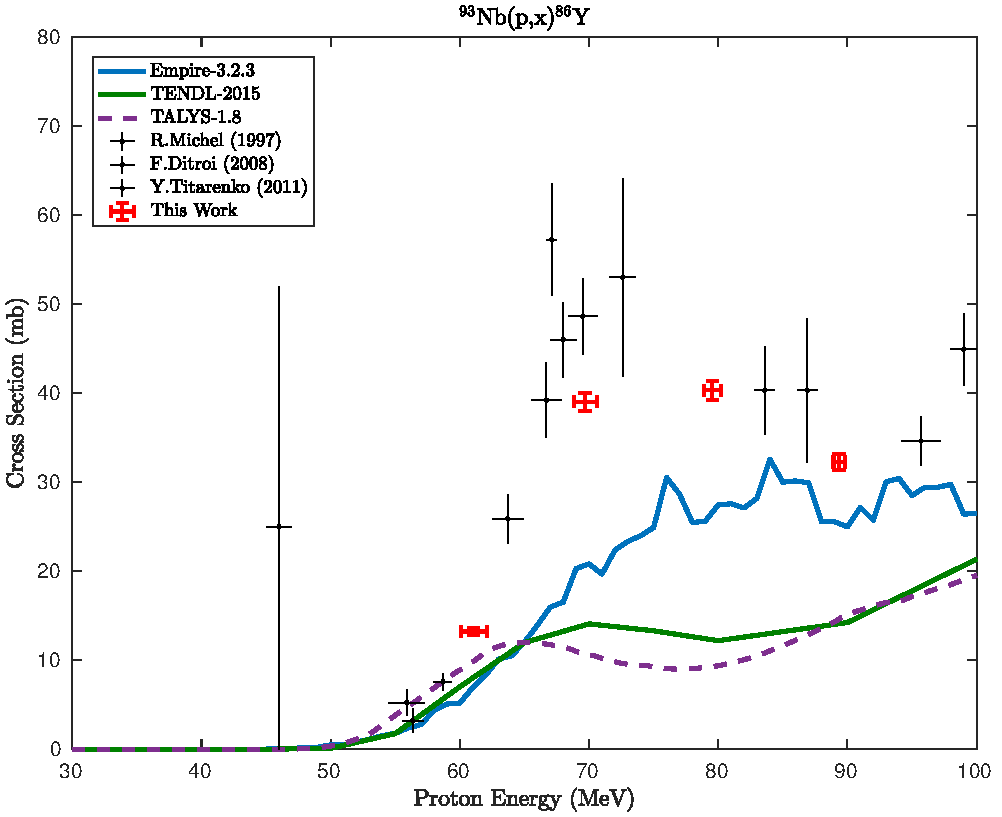
\includegraphics[width=0.5\linewidth]{./figures/86Y.pdf}
 % Nb_ptallies.pdf: 380x298 pixel, 72dpi, 13.41x10.51 cm, bb=0 0 380 298
 \caption{Measured \ce{^{93}Nb}(p,x)\ce{^{86}Y} cross section, with the \ce{^{93}Nb}(p,$\alpha$p3n)\ce{^{86}Y} reaction channel visibly peaking at approximately \mbox{70 MeV}.}
 \label{fig:86Y}
\end{figure}




\begin{figure}
 \centering
 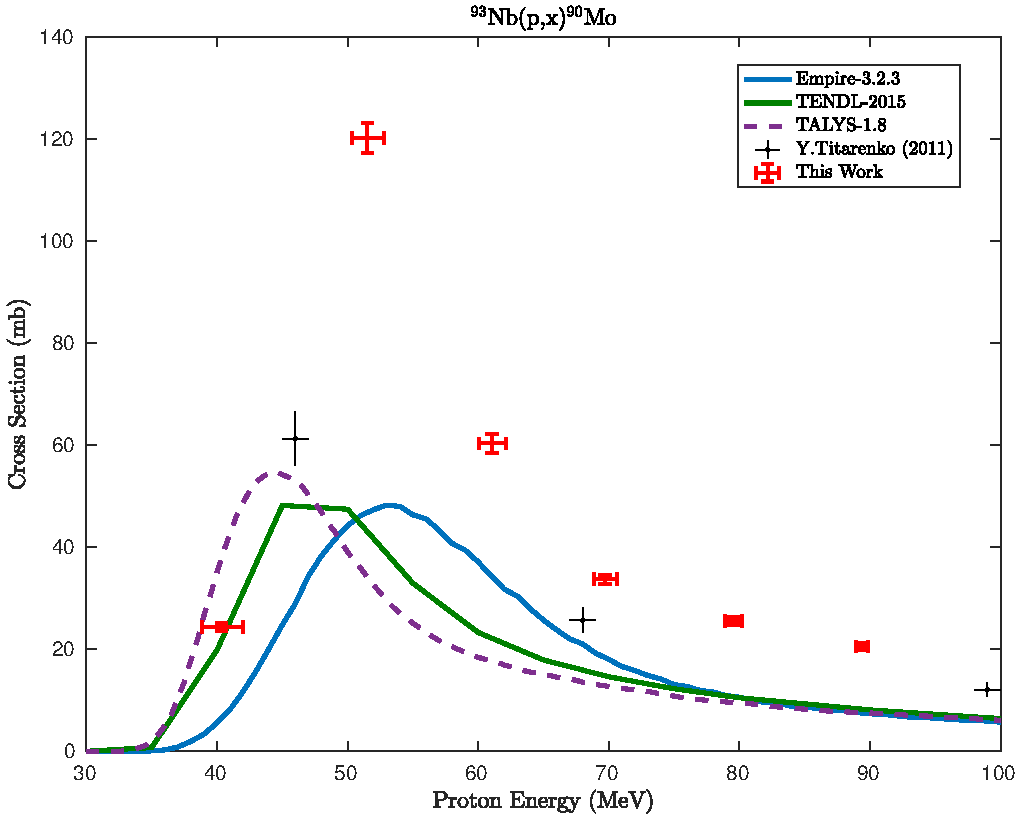
\includegraphics[width=0.5\linewidth]{./figures/90Mo.pdf}
 % Nb_ptallies.pdf: 380x298 pixel, 72dpi, 13.41x10.51 cm, bb=0 0 380 298
 \caption{Measured \ce{^{93}Nb}(p,x)\ce{^{90}Mo} cross section, with the \ce{^{93}Nb}(p,4n)\ce{^{90}Mo} reaction channel visibly peaking at approximately \mbox{50 MeV}.}
 \label{fig:90Mo}
\end{figure}


\begin{figure}
 \centering
 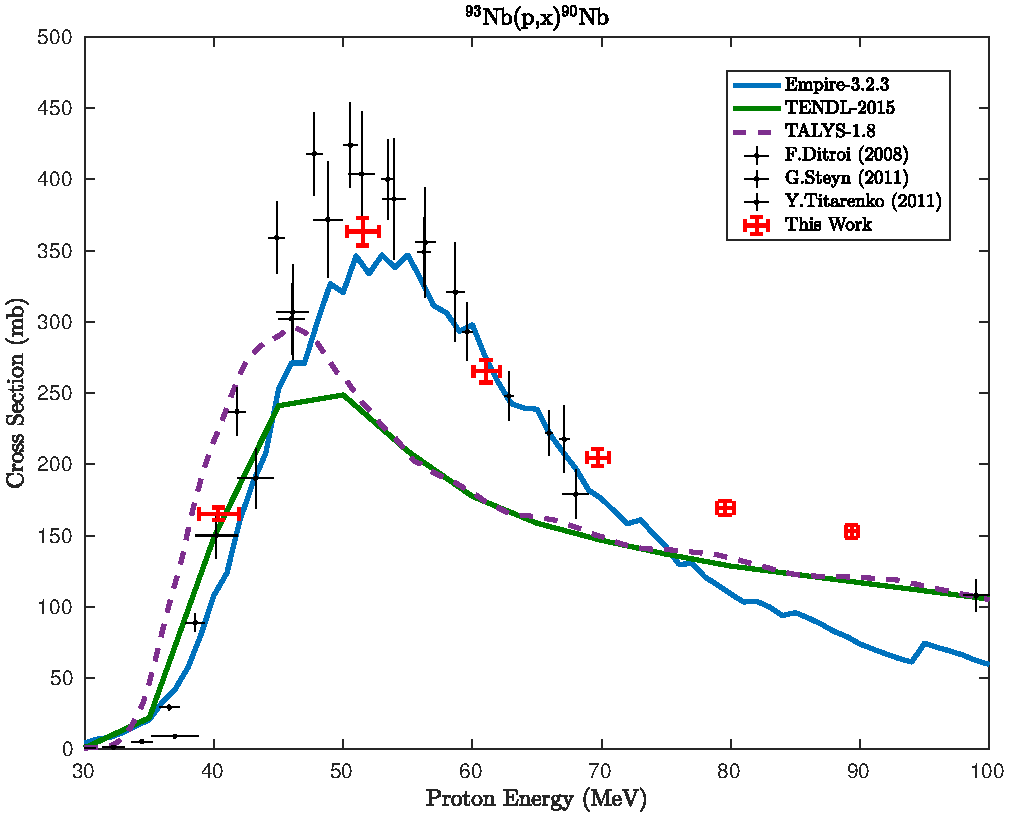
\includegraphics[width=0.5\linewidth]{./figures/90Nb.pdf}
 % Nb_ptallies.pdf: 380x298 pixel, 72dpi, 13.41x10.51 cm, bb=0 0 380 298
 \caption{Measured \ce{^{93}Nb}(p,x)\ce{^{90}Nb} cross section, with the \ce{^{93}Nb}(p,p3n)\ce{^{90}Nb} reaction channel visibly peaking at approximately \mbox{50 MeV}.}
 \label{fig:90Nb}
\end{figure}




In all three channels, the TALYS, TENDL, and CoH calculations rise, peak, and fall at lower energies than the data, while EMPIRE calculates the peak to occur at higher energies.
For \ce{^{90}Mo}, the EMPIRE peak is representative of the data.
For \ce{^{86}Y} and \ce{^{90}Nb}, the peak is missed by all three  of the codes.


The magnitudes of the TALYS and TENDL calculations are consistently too low in the three channels studied here. 
For \ce{^{86}Y}, CoH and EMPIRE also predict smaller cross sections than the data would suggest, which may be influenced by incorrect modeling of other, stronger, channels.
The magnitude of the peak in the CoH calculation for \ce{^{90}Mo}  is consistent  with the data, while EMPIRE predicts a cross section that is approximately the same magnitude as that of TALYS.
\ce{^{90}Nb} is one of the strongest measured channels, approximately 10\% of the total reaction cross section, and the three codes are all consistent, but  too small, in magnitude.

The \ce{^{90}Nb} production cross section exhibits a persistent pre-equilibrium \enquote{tail} that keeps the channel open  well after the compound cross section has fallen away. 
TALYS, TENDL, and CoH seem to have the correct shape for this pre-equilibrium cross section, with magnitudes that are just slightly too low.
EMPIRE, however, does not level off  as much as the data and the other codes are seen to, and misses the high-energy data points.

          
% \section{Discussion}

% \comment{Feel free to expand / suggest / add other language describing medical radionuclide applications, or radiochemical separations here.}


% \comment{Make sure to comment on avoiding the use of silicone-based adhesives for Al monitor foils.}

Finally, we wish to urge caution in future stacked-target activation experiments by avoiding the use of silicone adhesive-based tapes for foil containment, especially when paired with the use of Al monitor foils.
Acrylic-based tape options are commercially available, and are immune from (p,x) production of \ce{^{22,24}Na} activities, due to being of too low-Z for these reaction channels to be possible.
Even with subtraction of \ce{^{22,24}Na} activities though irradiating a Kapton tape \enquote{blank} or similar, we observe the Al monitor channels to measure consistently higher proton fluence than via Cu monitor channels, by 5--8\%. 
If Al monitors are used in conjunction with silicone-based tapes, even with subtraction of excess \ce{^{22}Na} activities, a systematically enhanced fluence may be determined, leading to cross sections reported with inaccurately diminished magnitude.
Furthermore, since data for monitor reactions are often self-referencing, the propagated impact of this systematic enhancement in fluence may have far-reaching consequences for both medical isotope production, as well as for  the evaluated nuclear data libraries, which use these proton activation experiments as input.

% First off, at the next planned stack irradiation at IPF, we would strongly encourage that a Kapton "blank" (no foil in the packet) be irradiated to confirm this.  We intend to do the same for our next proton irradiation at LBL.
% 
% We would highly encourage people to be careful about the small details, notably using a silicone-based adhesive for any future Al monitor foils.  This has potentially far-reaching consequences, unless a non-silicon-based Kapton (such as the acrylic adhesive versions) is instead used.


% XXXXXX
 
% \comment{Placeholder to reserve space for pre-equilibrium / spin discussion.} 
 
 
 
 \section{Conclusions}

We present here a set of 38 measurements of cross sections for the \ce{^{nat}Nb}(p,x) and  \ce{^{nat}Cu}(p,x) reactions between 40--90 MeV, as well as 5 independent measurements of isomer branching ratios.
Nearly all cross sections have been reported with higher precision than previous measurements.
We report the first measurements of the  \ce{^{nat}Nb}(p,x)\ce{^{82m}Rb} reaction, as well as the first measurement of the independent cross sections for    \ce{^{nat}Cu}(p,x)\ce{^{52\text{m}}Mn}, \ce{^{nat}Cu}(p,x)\ce{^{52\text{g}}Mn}, and \ce{^{nat}Nb}(p,x)\ce{^{85\text{g}}Y} in the 40--90 MeV region.
We also use these measurements to illustrate the impact of pre-equilibrium particle emission in the reaction dynamics for 40--90 MeV \ce{^{nat}Nb}(p,x) and  \ce{^{nat}Cu}(p,x) reactions.
We advise that future activation experiments avoid the use of silicone-based adhesives, particularly in conjunction with aluminum monitor foils, to avoid reporting an enhanced fluence due to \ce{^{22,24}Na} contamination.
Finally, this work provides another example of the usefulness of the recently-described variance minimization techniques for reducing energy uncertainties in stacked target charged particle irradiation experiments.



 
 \section{Acknowledgements}
 
%  Stephen Graves - consulting for methodology, guidance.
 
 The authors would like to particularly acknowledge the assistance and support of  Michael Gallegos and Don Dry in the LANL C-NR Countroom, David Reass and Mike Connors at LANSCE-IPF, and the LANSCE Accelerator Operations staff. 
 
We gratefully acknowledge support for this work from the United States Department of Energy, Office of Science via the Isotope Development and Production for Research and Applications subprogram in the Office of Nuclear Physics. 
This work has been carried out  under the auspices of the U.S. Department of Energy by  Lawrence Berkeley National Laboratory and the U.S. Nuclear Data Program under contract \# DE-AC02-05CH11231.
This research was performed under appointment to the Rickover Fellowship Program in Nuclear Engineering, sponsored by the Naval Reactors Division of the U.S. Department of Energy
Additional support has been provided by the U.S. Nuclear Regulatory Commission.



 
This research used the Savio computational cluster resource provided by the Berkeley Research Computing program at the University of California, Berkeley (supported by the UC Berkeley Chancellor, Vice Chancellor for Research, and Chief Information Officer).

 
%  This work has been carried out at the University of California, Berkeley, and performed under the auspices of the U.S. Department of Energy by Lawrence Livermore National Laboratory under contract \# DE-AC52-07NA27344 and Lawrence Berkeley National Laboratory under contract \# DE-AC02-05CH11231.
% Funding has been provided from the US Nuclear Regulatory Commission, the US Nuclear Data Program, the Berkeley Geochronology Center, NSF ARRA Grant \# EAR-0960138, the University of California Laboratory Fees Research Grant \# 12-LR-238745, and  DFG Research Fellowship \# RU 2065/1-1.

% This work has been carried out  under the auspices of the U.S. Department of Energy by  Lawrence Berkeley National Laboratory under contract \# DE-AC02-05CH11231.
% Funding has been provided from the US Nuclear Regulatory Commission and the US Nuclear Data Program.

 
 
%  \comment{Please provide me here with all relevant contract / grant / fellowship / funding ID numbers, as well as anyone else that you feel should be acknowledged here.}
 
%  We would like to particularly point out the crucial role played by Cory Waltz in the design and commissioning of the HFNG.
%  We wish to thank Marc Garland and Saed Mirzadeh for discussions regarding the use of neutron generators for isotope production.
%  We acknowledge Glenn Jones of G\&J Jones Enterprises of Dublin, CA for the construction  of the High Flux Neutron Generator. 
%  Lastly, we would like to acknowledge the students in the Nuclear Reactions and Radiation (NE102) laboratory course at UC Berkeley who participated in these experiments, including Joe Corvino, Nizelle Fajardo, Scott Parker and Evan Still.  
%  
%  This work has been carried out at the University of California, Berkeley, and performed under the auspices of the U.S. Department of Energy by Lawrence Livermore National Laboratory under contract \# DE-AC52-07NA27344 and Lawrence Berkeley National Laboratory under contract \# DE-AC02-05CH11231.
% Funding has been provided from the US Nuclear Regulatory Commission, the US Nuclear Data Program, the Berkeley Geochronology Center, NSF ARRA Grant \# EAR-0960138, the University of California Laboratory Fees Research Grant \# 12-LR-238745, and  DFG Research Fellowship \# RU 2065/1-1.



% \pagebreak
% 
% \onecolumn
% 
\appendix


\section{Decay data} \label{data}
% 
% % \begin{longtable}{|c|c|c|c|c|} 
% % \caption{My caption}
% % \label{tab:dummy}
% % % \begin{tabular}{|c|c|c|c|c|}
% %    \hline
% %  
% % \end{longtable}
% Table of decay data  for observed gamma-rays. 
The   lifetimes and gamma-ray branching ratios  listed in these tables were used for all calculations of measured cross sections reported in this work, and have been taken from the most recent edition of  Nuclear Data Sheets for each  mass chain  \cite{Basunia2015,Firestone2007,Wang2017,Dong2015,Dong2014,JUNDE2008787,Junde2011,Bhat1998,Nesaraja2010,BAGLIN2002,Browne2013,Zuber20151,NICHOLS2012973,Singh2007,Browne2010,Tuli2003,McCutchan2015,Singh2014,NEGRET20151,Johnson2015,McCutchan2014,Singh2013,Browne1997,Baglin2013,Baglin2012,Baglin2011}. 


% \comment{I had to remove about 30 of the lines I used from this table (removing the weakest lines in nuclides with even more lines than shown here, but never removing lines in nuclides with only 2 or less), as even splitting the data into 2 tables created tables too large to fit on a single page.  My purpose here was 1) to show that I used multiple lines to quantify each nuclide (increasing confidence in results), and 2) to list all the used \ce{^{90}Mo} lines, since they form the basis of it as a monitor.  Is this good as is, or should it be pared down even more?}


% Preview source code for paragraph 0

\begin{table}[ht]
\centering
\caption{Decay data for gamma-rays observed in \ce{^{nat}Al}(p,x) and \ce{^{nat}Cu}(p,x).}
\label{tab:nudat_table_monitors}
\begin{tabular}{@{}llll@{}}
\toprule
% \begin{tabular}{|c|c|c|c|}
% \hline 
Nuclide & Half-life & E$_\gamma$ (keV) & I$_\gamma$ (\%)\\
\midrule
\ce{^{22}Na} & 2.6018(22) y & 1274.537 & 99.940(14)\\
 
\ce{^{24}Na} & 14.997(12) h & 1368.626 & 99.9936(15)\\
 
\ce{^{51}Cr} & 27.704(3) d & 320.0824 & 9.910(10)\\
 
\ce{^{52m}Mn} & 21.1(2) m & 1434.0600 & 98.2(5)\\
 
\ce{^{52}Mn} & 5.591(3) d & 744.233 & 90.0(12)\\
 
 & 5.591(3) d & 935.544 & 94.5(13)\\
 
 & 5.591(3) d & 1246.278 & 4.21(7)\\
 
 & 5.591(3) d & 1434.092 & 100.0(14)\\
 
\ce{^{54}Mn} & 312.20(20) & 834.848 & 99.9760(10)\\
 
\ce{^{55}Co} & 17.53(3) h & 477.2 & 20.2(17)\\
 
 & 17.53(3) h & 931.1 & 75.0(35)\\
 
 & 17.53(3) h & 1316.6 & 7.1(3)\\
 
 & 17.53(3) h & 1408.5 & 16.9(8)\\
 
\ce{^{56}Ni} & 6.075(10) d & 158.38 & 98.8(10)\\
 
 & 6.075(10) d & 269.50 & 36.5(8)\\
 
 & 6.075(10) d & 480.44 & 36.5(8)\\
 
 & 6.075(10) d & 749.95 & 49.5(12)\\
 
 & 6.075(10) d & 811.85 & 86.0(9)\\
 
 & 6.075(10) d & 1561.80 & 14.0(6)\\
 
\ce{^{56}Co} & 77.236(26) d & 846.770 & 99.9399(2)\\
 
%  & 77.236(26) d & 977.372 & 1.421(6)\\
 
 & 77.236(26) d & 1037.843 & 14.05(4)\\
 
 & 77.236(26) d & 1238.288 & 66.46(12)\\
 
 & 77.236(26) d & 1360.212 & 4.283(12)\\
 
 & 77.236(26) d & 1771.357 & 15.41(6)\\
 
\ce{^{57}Ni} & 35.60(6) h & 127.164 & 16.7(5)\\
 
 & 35.60(6) h & 1377.63 & 81.7(24)\\
 
 & 35.60(6) h & 1757.55 & 5.75(20)\\
 
 & 35.60(6) h & 1919.52 & 12.3(4)\\
 
\ce{^{57}Co} & 271.74(6) d & 122.06065 & 85.60(17)\\
 
 & 271.74(6) d & 136.47356 & 10.68(8)\\
 
\ce{^{58}Co} & 70.86(6) d & 810.7593 & 99.450(10)\\
 
 & 70.86(6) d & 863.951 & 0.686(10)\\
 
%  & 70.86(6) d & 1674.725 & 0.517(10)\\
 
\ce{^{59}Fe} & 44.495(9) d & 1099.245 & 56.5(18)\\
 
 & 44.495(9) d & 1291.590 & 43.2(14)\\
 
\ce{^{60}Co} & 5.2714(5) y & 1173.228 & 99.85(3)\\
 
 & 5.2714(5) y & 1332.492 & 99.9826(6)\\
 
\ce{^{61}Cu} & 3.339(8) h & 282.956 & 12.2(2.2)\\
 
 & 3.339(8) h & 373.050 & 2.1(4)\\
 
%  & 3.339(8) h & 588.605 & 1.17(21)\\
 
 & 3.339(8) h & 656.008 & 10.8(20)\\
 
 & 3.339(8) h & 1185.234 & 3.7(7)\\
 
\ce{^{62}Zn} & 9.193(15) h & 243.36 & 2.52(23)\\
 
 & 9.193(15) h & 246.95 & 1.90(18)\\
 
 & 9.193(15) h & 260.43 & 1.35(13)\\
 
%  & 9.193(15) h & 304.88 & 0.29(3)\\
 
%  & 9.193(15) h & 349.60 & 0.45(4)\\
 
 & 9.193(15) h & 394.03 & 2.24(17)\\
 
 & 9.193(15) h & 548.35 & 15.3(14)\\
 
 & 9.193(15) h & 596.56 & 26.0(20)\\
 
%  & 9.193(15) h & 637.41 & 0.25(3)\\
 
\ce{^{64}Cu} & 12.701(2) h & 1345.77 & 0.475(11)\\
 
\ce{^{65}Zn} & 243.93(9) d & 1115.539 & 50.04(10)\\
\bottomrule
\end{tabular}
\end{table}



\begin{table}[ht]
\centering
\caption{Decay data for gamma-rays observed in \ce{^{nat}Nb}(p,x).}
\label{tab:nudat_table_nb}
\begin{tabular}{@{}llll@{}}
\toprule
% \begin{tabular}{|c|c|c|c|}
% \hline 
Nuclide & Half-life & E$_\gamma$ (keV) & I$_\gamma$ (\%)\\
\midrule
\ce{^{82m}Rb} & 6.472(6) h & 554.35 & 62.4(9)\\
 
 & 6.472(6) h & 619.11 & 37.98(9)\\
 
%  & 6.472(6) h & 698.37 & 26.3(7)\\
 
 & 6.472(6) h & 776.52 & 84.39(21)\\
 
 & 6.472(6) h & 1044.08 & 32.07(8)\\
 
%  & 6.472(6) h & 1317.43 & 23.7(6)\\
 
\ce{^{83}Sr} & 32.41(3) h & 418.37 & 4.2(3)\\
 
 & 32.41(3) h & 762.65 & 26.7(22)\\
 
\ce{^{85m}Y} & 4.86(13) h & 231.7 & 22.8(22)\\
 
\ce{^{85}Y} & 2.68(5) h & 231.65 & 84(9)\\
 
 & 2.68(5) h & 913.89 & 9.0(9)\\
 
\ce{^{86}Zr} & 16.5(1) h & 242.8 & 95.84(2)\\
 
 & 16.5(1) h & 612.0 & 5.8(3)\\
 
% \ce{^{86}Y} & 14.74(2) h & 187.87 & 1.26(4)\\
\ce{^{86}Y}  & 14.74(2) h & 443.13 & 16.9(5)\\

 
%  & 14.74(2) h & 190.80 & 1.01(3)\\
 
%  & 14.74(2) h & 307.00 & 3.47(8)\\
 
%  & 14.74(2) h & 443.13 & 16.9(5)\\
 
%  & 14.74(2) h & 580.57 & 4.78(14)\\
 
%  & 14.74(2) h & 608.29 & 2.01(15)\\
 
 & 14.74(2) h & 627.72 & 32.6(1)\\
 
%  & 14.74(2) h & 703.33 & 15.4(4)\\
 
%  & 14.74(2) h & 709.90 & 2.62(8)\\
 
%  & 14.74(2) h & 767.63 & 2.4(3)\\
 
%  & 14.74(2) h & 835.67 & 4.4(6)\\
 
%  & 14.74(2) h & 1024.04 & 3.79(17)\\
 
 & 14.74(2) h & 1076.63 & 82.5(4)\\
 
 & 14.74(2) h & 1153.05 & 30.5(9)\\
 
%  & 14.74(2) h & 1163.03 & 1.18(4)\\
%  
%  & 14.74(2) h & 1253.11 & 1.53(5)\\
 
%  & 14.74(2) h & 1349.15 & 2.95(9)\\
 
 & 14.74(2) h & 1854.38 & 17.2(5)\\
 
 & 14.74(2) h & 1920.72 & 20.8(7)\\
 
\ce{^{87}Zr} & 1.68(1) h & 380.79 & 62.79(10)\\
 
 & 1.68(1) h & 1227.0 & 2.80(4)\\
 
\ce{^{87m}Y} & 13.37(1) h & 380.79 & 78.05(8)\\
 
\ce{^{87}Y} & 79.8(3) h & 388.5276 & 82.2(7)\\
 
 & 79.8(3) h & 484.805 & 89.8(9)\\
 
\ce{^{88}Zr} & 83.4(3) d & 392.87 & 97.29(14)\\
 
\ce{^{88}Y} & 106.627(21) d & 898.042 & 93.7(3)\\
 
 & 106.627(21) d & 1836.063 & 99.2(3)\\
 
\ce{^{89m}Nb} & 66(2) m & 588.0 & 95.57(13)\\
 
\ce{^{89}Nb} & 2.03(7) h & 1511.4 & 1.9(4)\\
 
 & 2.03(7) h & 1627.2 & 3.5(7)\\
 
 & 2.03(7) h & 1833.4 & 3.3(7)\\
 
\ce{^{89}Zr} & 78.41(12) h & 909.15 & 99.04(3)\\
 
 & 78.41(12) h & 1713.0 & 0.745(13)\\
 
%  & 78.41(12) h & 1744.5 & 0.123(4)\\
 
\ce{^{90}Mo} & 5.56(9) h & 122.370 & 64(3)\\
 
 & 5.56(9) h & 162.93 & 6.0(6)\\
 
 & 5.56(9) h & 203.13 & 6.4(6)\\
 
 & 5.56(9) h & 257.34 & 78(4)\\
 
 & 5.56(9) h & 323.20 & 6.3(6)\\
 
 & 5.56(9) h & 472.2 & 1.42(16)\\
 
 & 5.56(9) h & 941.5 & 5.5(7)\\
 
\ce{^{90}Nb} & 14.6(5) h & 132.716 & 4.13(4)\\
 
 & 14.6(5) h & 141.178 & 66.8(7)\\
 
%  & 14.6(5) h & 890.64 & 1.80(4)\\
 
 & 14.6(5) h & 1611.76 & 2.38(7)\\
 
%  & 14.6(5) h & 1913.194 & 1.280(17)\\
 
\ce{^{91m}Nb} & 60.86(22) d & 104.62 & 0.574(1)\\
 
 & 60.86(22) d & 1204.67 & 2.0(3)\\
 
\ce{^{92m}Nb} & 10.15(2) d & 912.6 & 1.78(10)\\
 
 & 10.15(2) d & 934.44 & 99.15(4)\\
 
\ce{^{93m}Mo} & 6.85(7) d & 263.049 & 57.4(11)\\
 
 & 6.85(7) d & 684.693 & 99.9(8)\\
 
 & 6.85(7) d & 1477.138 & 99.1(11)\\
\bottomrule
\end{tabular}
\end{table}


% 
% 
\section{Measured excitation functions} \label{fit_figures}

Figures of the cross sections measured in this work are presented here, in comparison with literature data \cite{Albouy1963,PhysRev.162.1055,PhysRevC.6.1235,Grutter1982,Greenwood1984,Aleksandrov1987,levkovski1991cross,Mills1992,MICHEL1997153,Fassbender1997,Ido2002,sisterson2002selected,YashimaH2003,A2006,Ditroi2008,Ditroi2009,steyn2011excitation,Titarenko2011,Shahid2015,Garrido2016,Graves2016}, the TENDL-2015 data library \cite{Koning2012}, and the reaction modeling codes CoH-3.5.1, EMPIRE-3.2.3, and TALYS-1.8 \cite{KAWANO2010,Herman2007,Koning2012}.

% \comment{Add in CoH model output from Toshihiko to all plots}




% \comment{Fix a few figure labels (c/i) based on Jon;s email}



\begin{figure*}
    \centering
    \begin{subfigure}[t]{0.495\textwidth}
        \centering
%         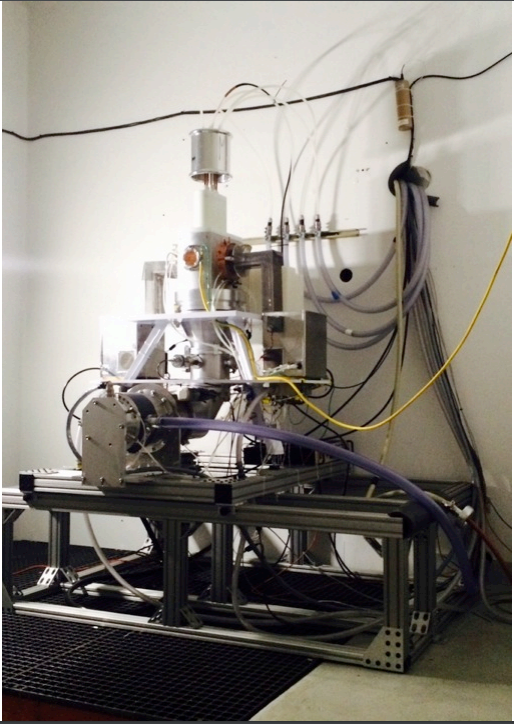
\includegraphics[width=\columnwidth]{./figures/Capture.PNG}
        \subfigimg[width=\linewidth]{}{./figures/51Cr.pdf}{50}
%         \caption{ Decay curve for the isomeric transition of \ce{^{115m}In}.}
         \refstepcounter{subfigure}\label{fig:51Cr}
    \end{subfigure}%
     \begin{subfigure}[t]{0.495\textwidth}
        \centering
%         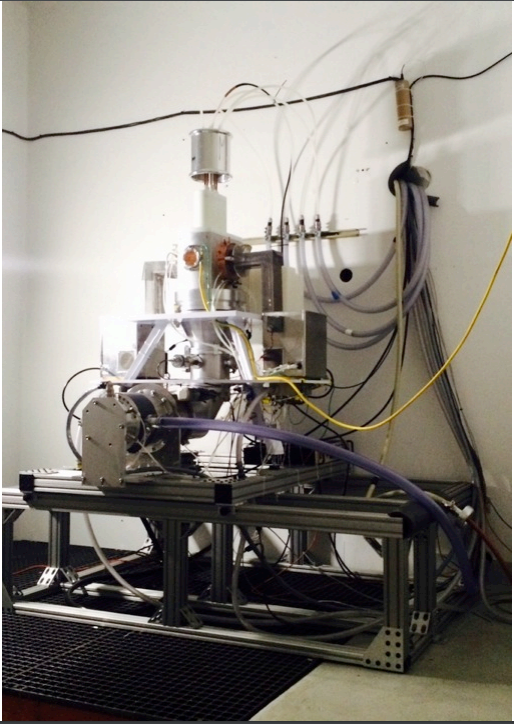
\includegraphics[width=\columnwidth]{./figures/Capture.PNG}
%         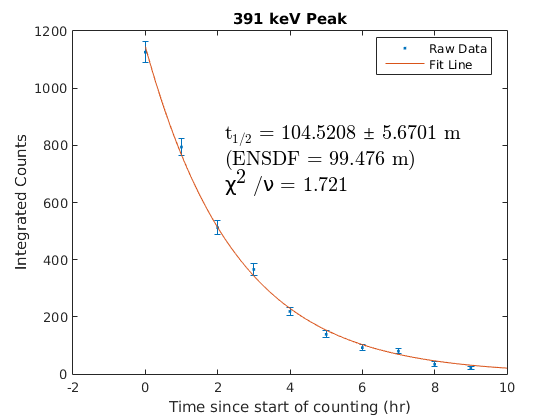
\includegraphics[scale=0.6]{./figures/391keV_curve2.png}
        \subfigimg[width=\linewidth]{}{./figures/52Mn.pdf}{50}
%         \caption{ Decay curve for the isomeric transition of \ce{^{113m}In}.}
         \refstepcounter{subfigure}\label{fig:52Mn}
    \end{subfigure}%
    \\
    \begin{subfigure}[t]{0.495\textwidth}
        \centering
%         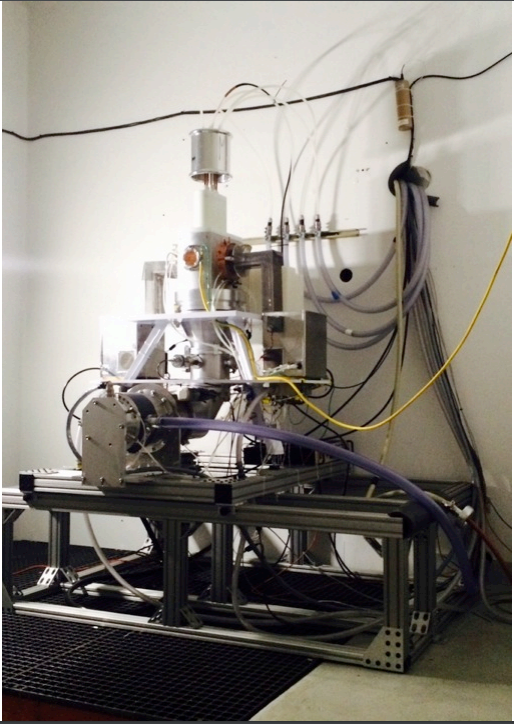
\includegraphics[width=\columnwidth]{./figures/Capture.PNG}
        \subfigimg[width=\linewidth]{}{./figures/52gMn.pdf}{50}
%         \caption{ Decay curve for the isomeric transition of \ce{^{115m}In}.}
         \refstepcounter{subfigure}\label{fig:52gMn}
    \end{subfigure}%
     \begin{subfigure}[t]{0.495\textwidth}
        \centering
%         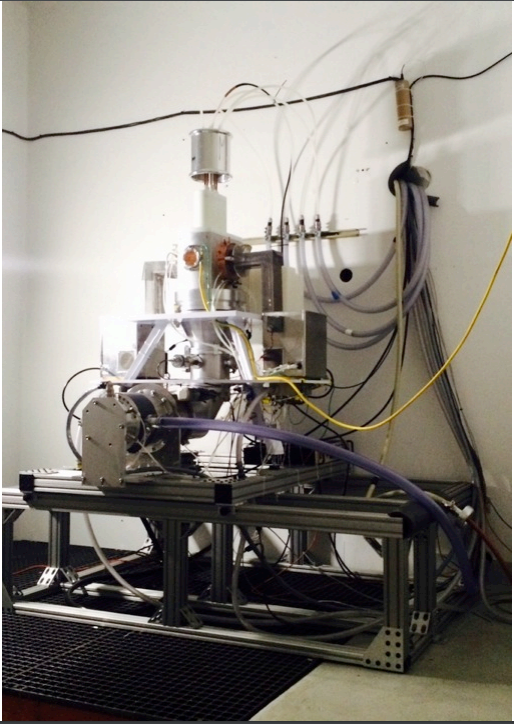
\includegraphics[width=\columnwidth]{./figures/Capture.PNG}
%         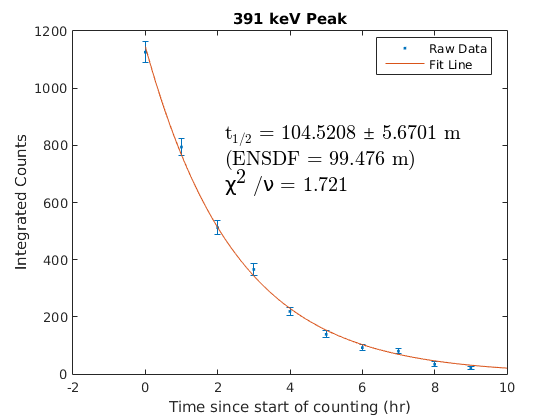
\includegraphics[scale=0.6]{./figures/391keV_curve2.png}
        \subfigimg[width=\linewidth]{}{./figures/52mMn.pdf}{50}
%         \caption{ Decay curve for the isomeric transition of \ce{^{113m}In}.}
         \refstepcounter{subfigure}\label{fig:52mMn}
    \end{subfigure}%
    \\
    \begin{subfigure}[t]{0.495\textwidth}
        \centering
%         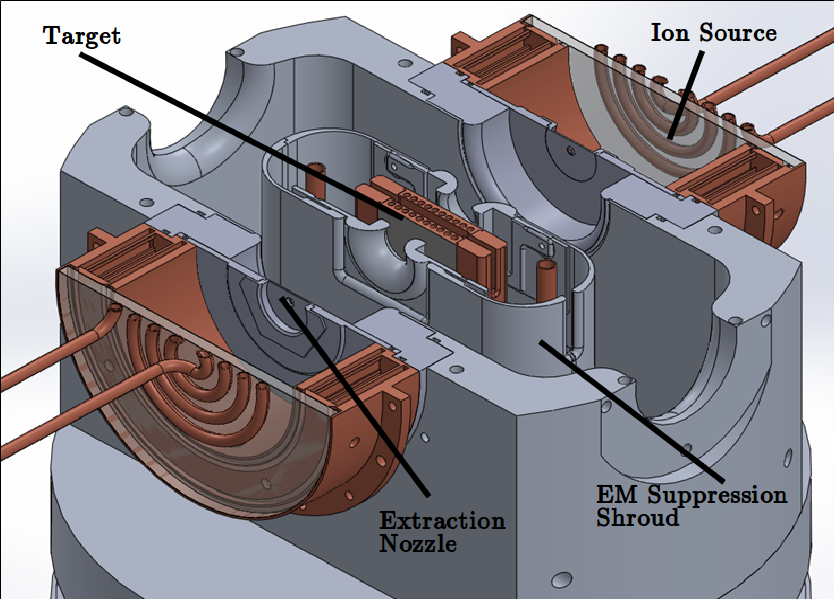
\includegraphics[width=\textwidth]{./figures/target2.png}
        \subfigimg[width=\linewidth]{}{./figures/54Mn.pdf}{50}
%         \caption{Decay curve for the $\beta^-$ decay of \ce{^{116}In}.}
                 \refstepcounter{subfigure}\label{fig:54Mn}
    \end{subfigure}
     \begin{subfigure}[t]{0.495\textwidth}
        \centering
%         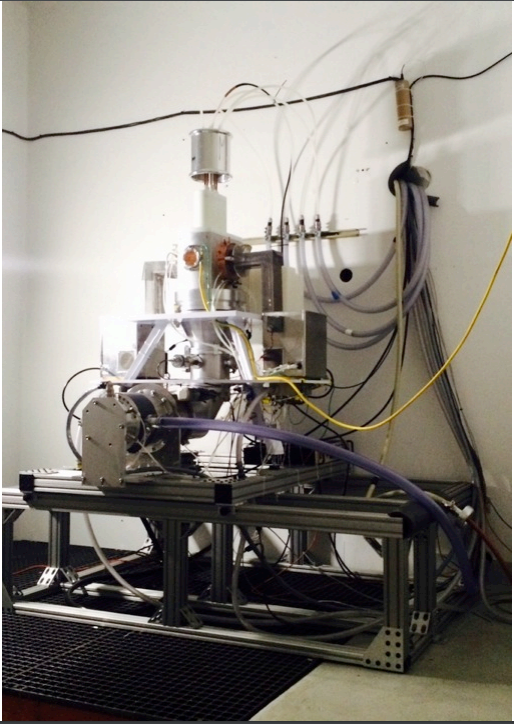
\includegraphics[width=\columnwidth]{./figures/Capture.PNG}
        \subfigimg[width=\linewidth]{}{./figures/55Co.pdf}{50}
%         \caption{ Decay curve for the $\beta^+$ decay of \ce{^{64}Cu}.}
        \refstepcounter{subfigure} \label{fig:55Co}
    \end{subfigure}%
%     \caption{Decay curves used to verify photopeak transition assignment. (a) Decay curve for the isomeric transition of \ce{^{115m}In}, (b) decay curve for the isomeric transition of \ce{^{113m}In}, (c) decay curve for the $\beta^-$ decay of \ce{^{116}In}, and (d) decay curve for the $\beta^+$ decay of \ce{^{64}Cu}.}
     \label{fig:xs_curves_p1}
\end{figure*}




\begin{figure*}
    \centering
    \begin{subfigure}[t]{0.495\textwidth}
        \centering
%         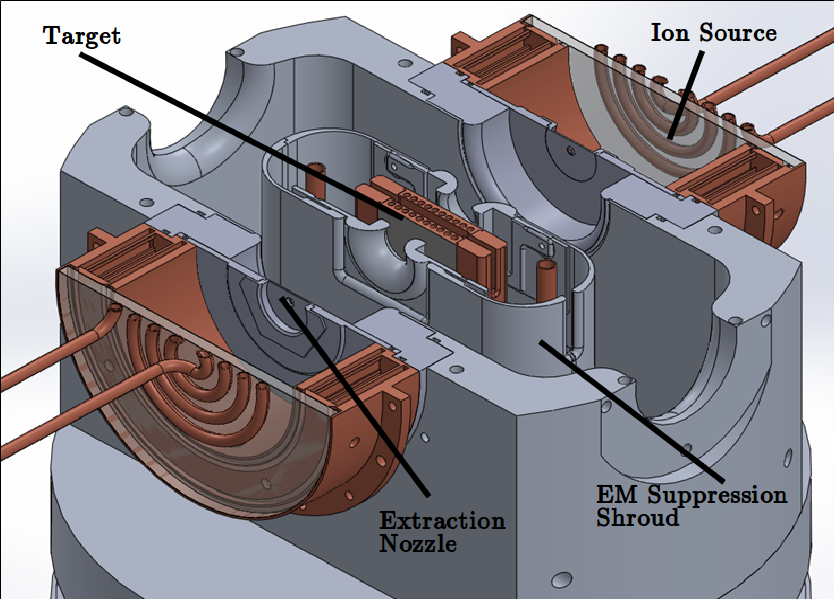
\includegraphics[width=\textwidth]{./figures/target2.png}
        \subfigimg[width=\linewidth]{}{./figures/56Ni.pdf}{50}
%         \caption{Decay curve for the $\beta^-$ decay of \ce{^{116}In}.}
                 \refstepcounter{subfigure}\label{fig:56Ni}
    \end{subfigure}
     \begin{subfigure}[t]{0.495\textwidth}
        \centering
%         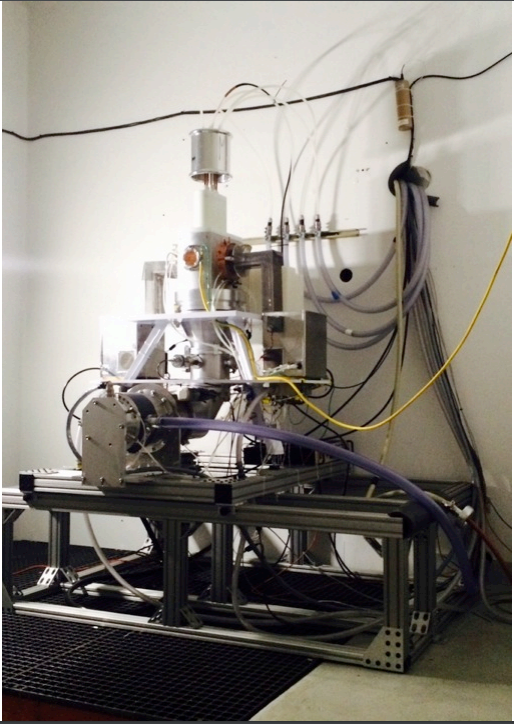
\includegraphics[width=\columnwidth]{./figures/Capture.PNG}
        \subfigimg[width=\linewidth]{}{./figures/57Co.pdf}{50}
%         \caption{ Decay curve for the $\beta^+$ decay of \ce{^{64}Cu}.}
        \refstepcounter{subfigure} \label{fig:57Co}
    \end{subfigure}%
    \\
    \begin{subfigure}[t]{0.495\textwidth}
        \centering
%         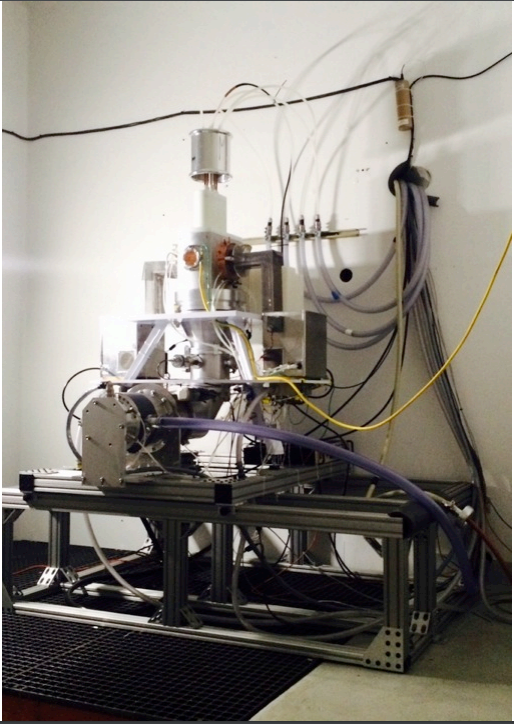
\includegraphics[width=\columnwidth]{./figures/Capture.PNG}
        \subfigimg[width=\linewidth]{}{./figures/57Ni.pdf}{50}
%         \caption{ Decay curve for the isomeric transition of \ce{^{115m}In}.}
         \refstepcounter{subfigure}\label{fig:57Ni}
    \end{subfigure}%
     \begin{subfigure}[t]{0.495\textwidth}
        \centering
%         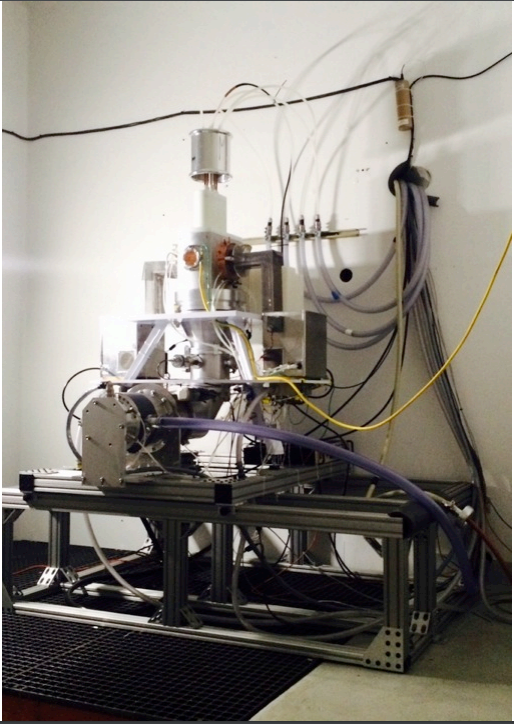
\includegraphics[width=\columnwidth]{./figures/Capture.PNG}
%         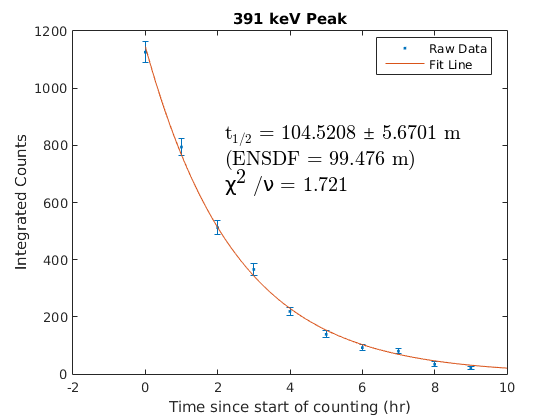
\includegraphics[scale=0.6]{./figures/391keV_curve2.png}
        \subfigimg[width=\linewidth]{}{./figures/58Co.pdf}{50}
%         \caption{ Decay curve for the isomeric transition of \ce{^{113m}In}.}
         \refstepcounter{subfigure}\label{fig:58Co}
    \end{subfigure}%
    \\
    \begin{subfigure}[t]{0.495\textwidth}
        \centering
%         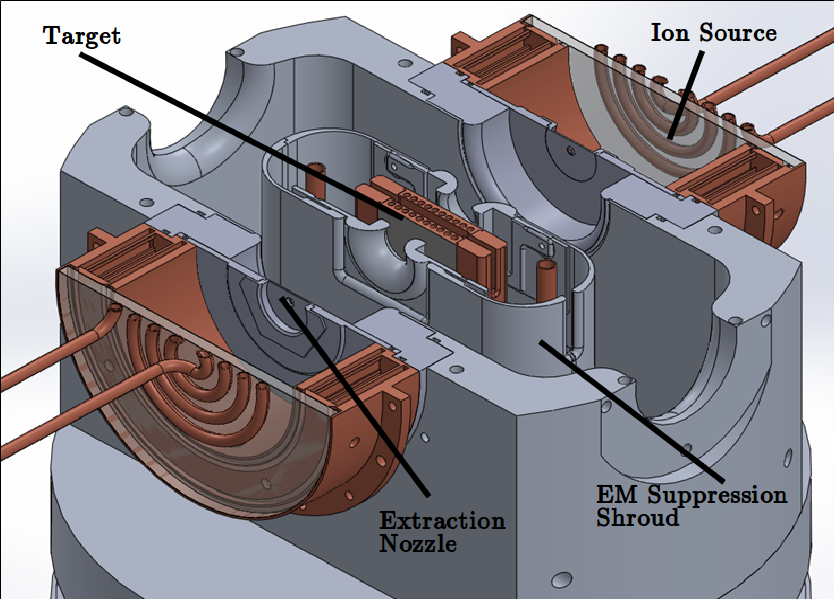
\includegraphics[width=\textwidth]{./figures/target2.png}
        \subfigimg[width=\linewidth]{}{./figures/58gCo.pdf}{50}
%         \caption{Decay curve for the $\beta^-$ decay of \ce{^{116}In}.}
                 \refstepcounter{subfigure}\label{fig:58gCo}
    \end{subfigure}
     \begin{subfigure}[t]{0.495\textwidth}
        \centering
%         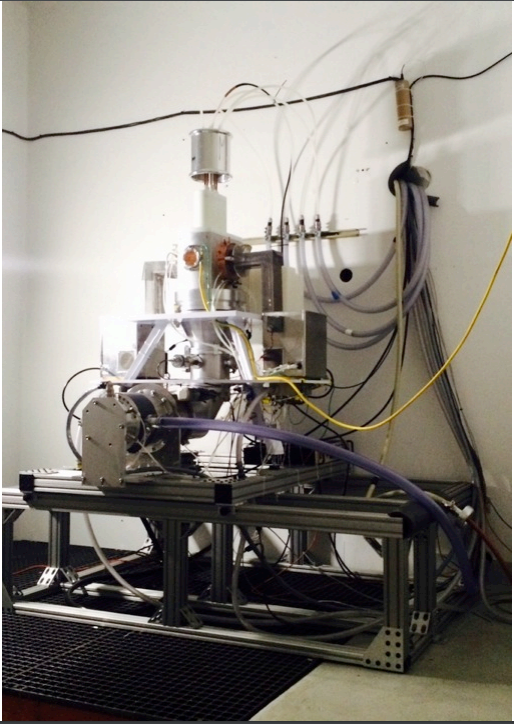
\includegraphics[width=\columnwidth]{./figures/Capture.PNG}
        \subfigimg[width=\linewidth]{}{./figures/58mCo.pdf}{50}
%         \caption{ Decay curve for the $\beta^+$ decay of \ce{^{64}Cu}.}
        \refstepcounter{subfigure} \label{fig:58mCo}
    \end{subfigure}%
%     \caption{Decay curves used to verify photopeak transition assignment. (a) Decay curve for the isomeric transition of \ce{^{115m}In}, (b) decay curve for the isomeric transition of \ce{^{113m}In}, (c) decay curve for the $\beta^-$ decay of \ce{^{116}In}, and (d) decay curve for the $\beta^+$ decay of \ce{^{64}Cu}.}
     \label{fig:xs_curves_p2}
\end{figure*}



\begin{figure*}
    \centering
    \begin{subfigure}[t]{0.495\textwidth}
        \centering
%         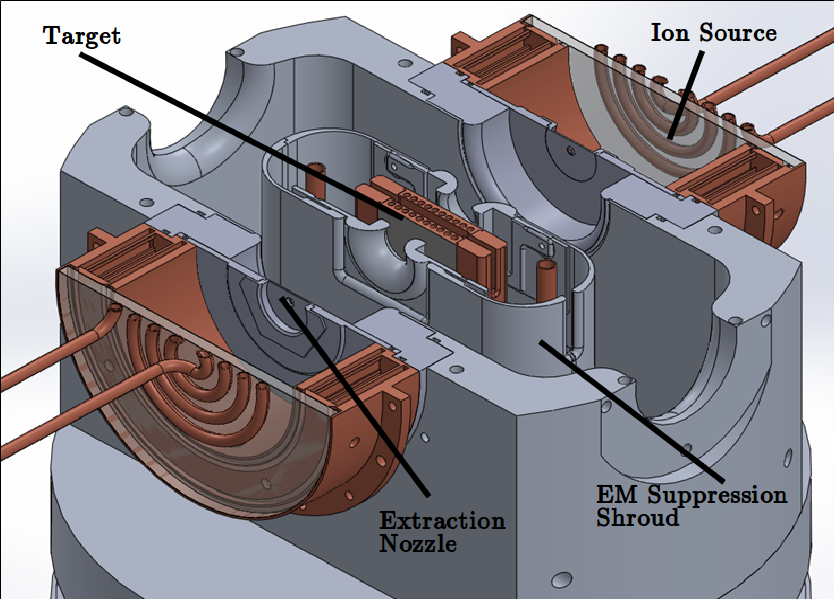
\includegraphics[width=\textwidth]{./figures/target2.png}
        \subfigimg[width=\linewidth]{}{./figures/59Fe.pdf}{50}
%         \caption{Decay curve for the $\beta^-$ decay of \ce{^{116}In}.}
                 \refstepcounter{subfigure}\label{fig:59Fe}
    \end{subfigure}
     \begin{subfigure}[t]{0.495\textwidth}
        \centering
%         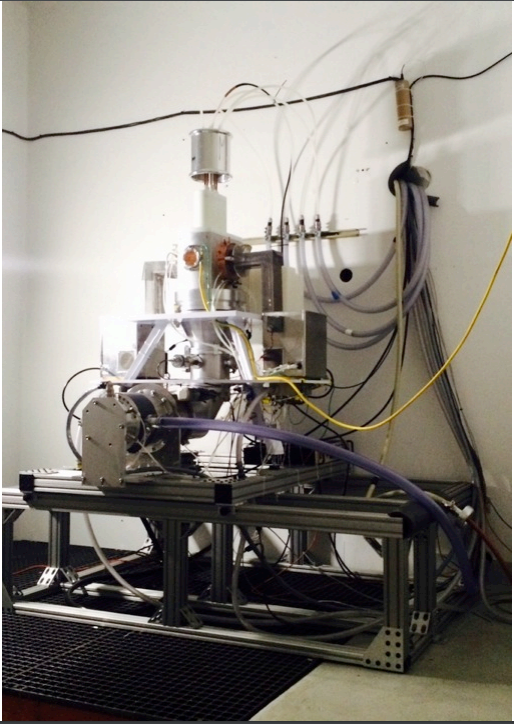
\includegraphics[width=\columnwidth]{./figures/Capture.PNG}
        \subfigimg[width=\linewidth]{}{./figures/60Co.pdf}{50}
%         \caption{ Decay curve for the $\beta^+$ decay of \ce{^{64}Cu}.}
        \refstepcounter{subfigure} \label{fig:60Co}
    \end{subfigure}%
    \\
    \begin{subfigure}[t]{0.495\textwidth}
        \centering
%         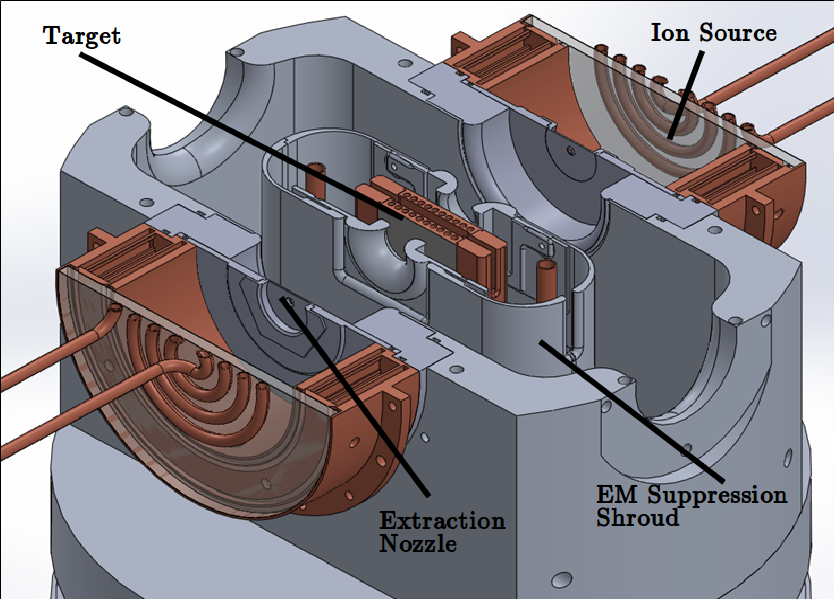
\includegraphics[width=\textwidth]{./figures/target2.png}
        \subfigimg[width=\linewidth]{}{./figures/61Cu.pdf}{50}
%         \caption{Decay curve for the $\beta^-$ decay of \ce{^{116}In}.}
                 \refstepcounter{subfigure}\label{fig:61Cu}
    \end{subfigure}
     \begin{subfigure}[t]{0.495\textwidth}
        \centering
%         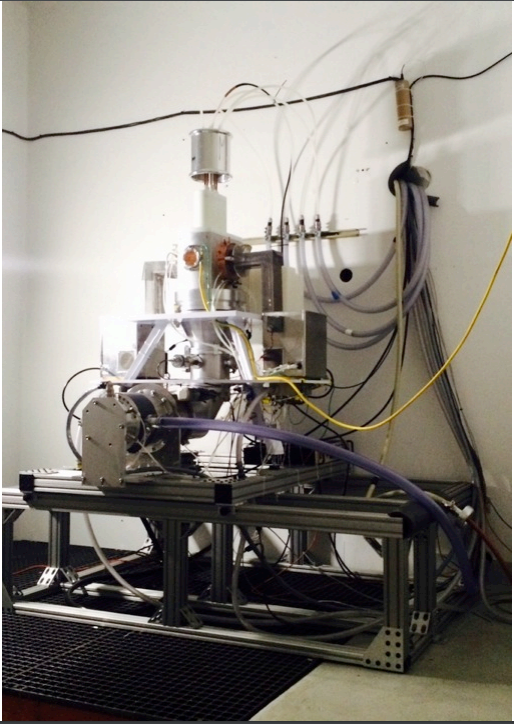
\includegraphics[width=\columnwidth]{./figures/Capture.PNG}
        \subfigimg[width=\linewidth]{}{./figures/64Cu.pdf}{50}
%         \caption{ Decay curve for the $\beta^+$ decay of \ce{^{64}Cu}.}
        \refstepcounter{subfigure} \label{fig:64Cu}
    \end{subfigure}%
    \\
    \begin{subfigure}[t]{0.495\textwidth}
        \centering
%         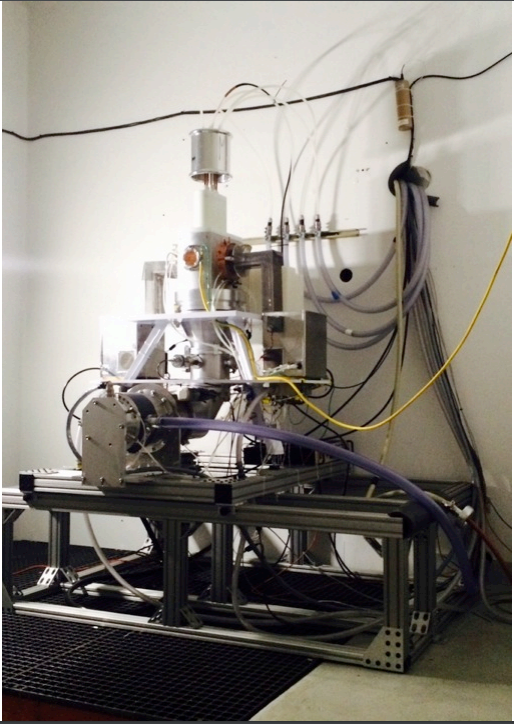
\includegraphics[width=\columnwidth]{./figures/Capture.PNG}
        \subfigimg[width=\linewidth]{}{./figures/82mRb.pdf}{50}
%         \caption{ Decay curve for the isomeric transition of \ce{^{115m}In}.}
         \refstepcounter{subfigure}\label{fig:82mRb}
    \end{subfigure}%
     \begin{subfigure}[t]{0.495\textwidth}
        \centering
%         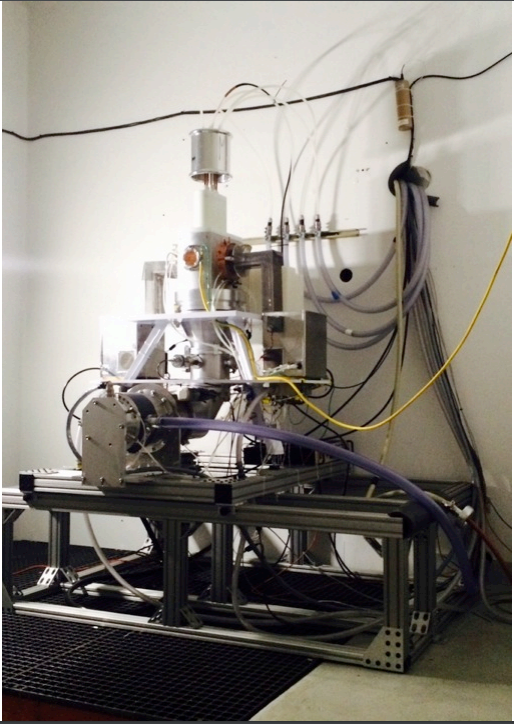
\includegraphics[width=\columnwidth]{./figures/Capture.PNG}
%         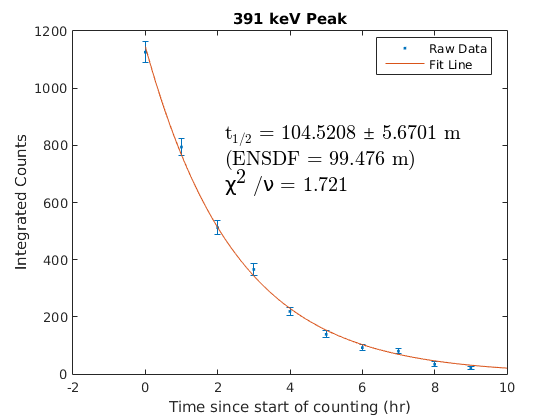
\includegraphics[scale=0.6]{./figures/391keV_curve2.png}
        \subfigimg[width=\linewidth]{}{./figures/83Sr.pdf}{50}
%         \caption{ Decay curve for the isomeric transition of \ce{^{113m}In}.}
         \refstepcounter{subfigure}\label{fig:83Sr}
    \end{subfigure}%
%     \caption{Decay curves used to verify photopeak transition assignment. (a) Decay curve for the isomeric transition of \ce{^{115m}In}, (b) decay curve for the isomeric transition of \ce{^{113m}In}, (c) decay curve for the $\beta^-$ decay of \ce{^{116}In}, and (d) decay curve for the $\beta^+$ decay of \ce{^{64}Cu}.}
     \label{fig:xs_curves_p3}
\end{figure*}



\begin{figure*}
    \centering
    \begin{subfigure}[t]{0.495\textwidth}
        \centering
%         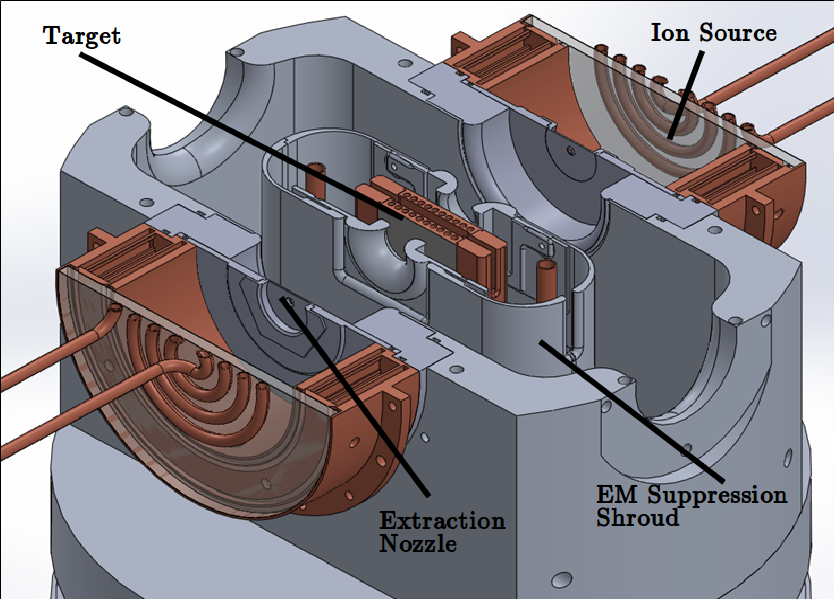
\includegraphics[width=\textwidth]{./figures/target2.png}
        \subfigimg[width=\linewidth]{}{./figures/85Y.pdf}{50}
%         \caption{Decay curve for the $\beta^-$ decay of \ce{^{116}In}.}
                 \refstepcounter{subfigure}\label{fig:85Y}
    \end{subfigure}
     \begin{subfigure}[t]{0.495\textwidth}
        \centering
%         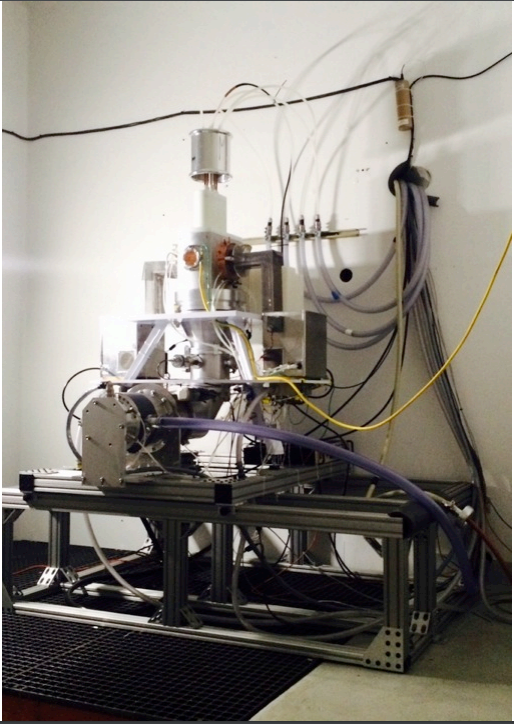
\includegraphics[width=\columnwidth]{./figures/Capture.PNG}
        \subfigimg[width=\linewidth]{}{./figures/85gY.pdf}{50}
%         \caption{ Decay curve for the $\beta^+$ decay of \ce{^{64}Cu}.}
        \refstepcounter{subfigure} \label{fig:85gY}
    \end{subfigure}%
    \\
    \begin{subfigure}[t]{0.495\textwidth}
        \centering
%         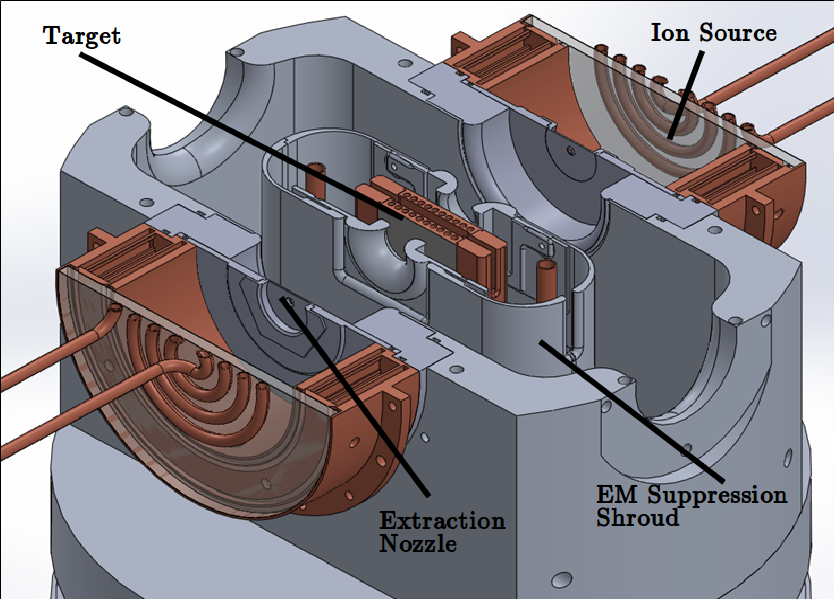
\includegraphics[width=\textwidth]{./figures/target2.png}
        \subfigimg[width=\linewidth]{}{./figures/85mY.pdf}{50}
%         \caption{Decay curve for the $\beta^-$ decay of \ce{^{116}In}.}
                 \refstepcounter{subfigure}\label{fig:85mY}
    \end{subfigure}
%      \begin{subfigure}[t]{0.495\textwidth}
%         \centering
% %         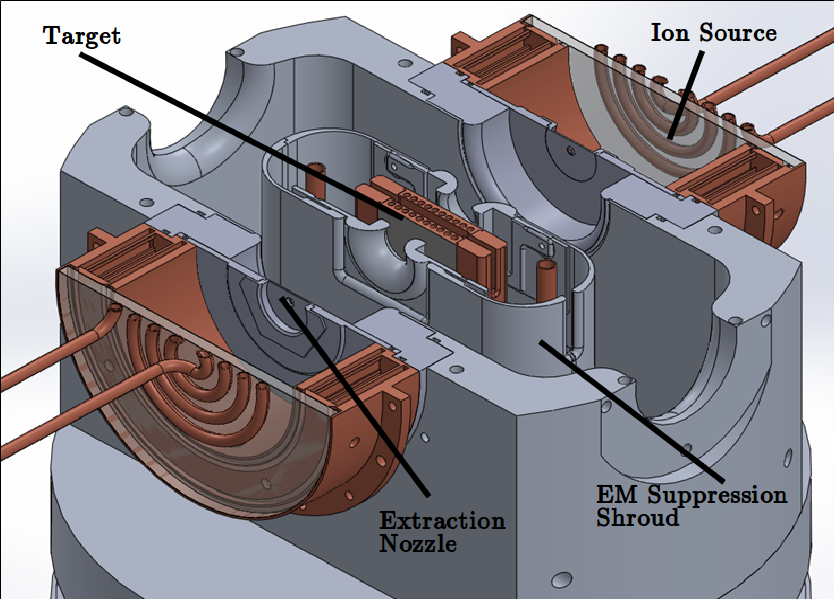
\includegraphics[width=\textwidth]{./figures/target2.png}
%         \subfigimg[width=\linewidth]{}{./figures/86Y.pdf}{50}
% %         \caption{Decay curve for the $\beta^-$ decay of \ce{^{116}In}.}
%                  \refstepcounter{subfigure}\label{fig:86Y}
%     \end{subfigure}
%     \\
    \begin{subfigure}[t]{0.495\textwidth}
        \centering
%         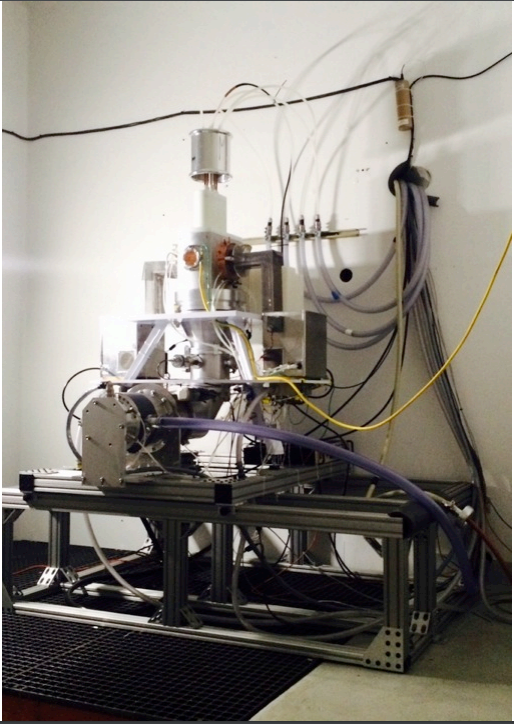
\includegraphics[width=\columnwidth]{./figures/Capture.PNG}
        \subfigimg[width=\linewidth]{}{./figures/86Zr.pdf}{50}
%         \caption{ Decay curve for the $\beta^+$ decay of \ce{^{64}Cu}.}
        \refstepcounter{subfigure} \label{fig:86Zr}
    \end{subfigure}%
    \\
    \begin{subfigure}[t]{0.495\textwidth}
        \centering
%         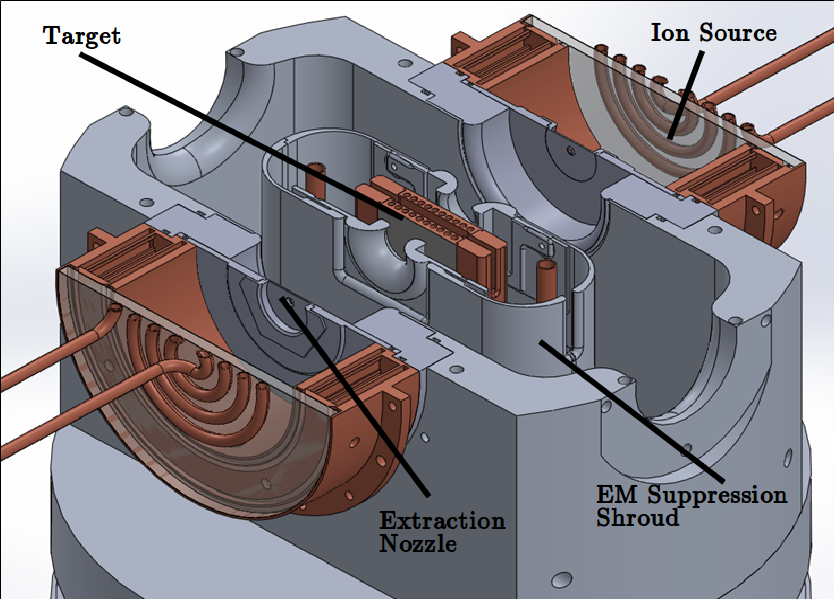
\includegraphics[width=\textwidth]{./figures/target2.png}
        \subfigimg[width=\linewidth]{}{./figures/87Y.pdf}{50}
%         \caption{Decay curve for the $\beta^-$ decay of \ce{^{116}In}.}
                 \refstepcounter{subfigure}\label{fig:87Y}
    \end{subfigure}
    \begin{subfigure}[t]{0.495\textwidth}
        \centering
%         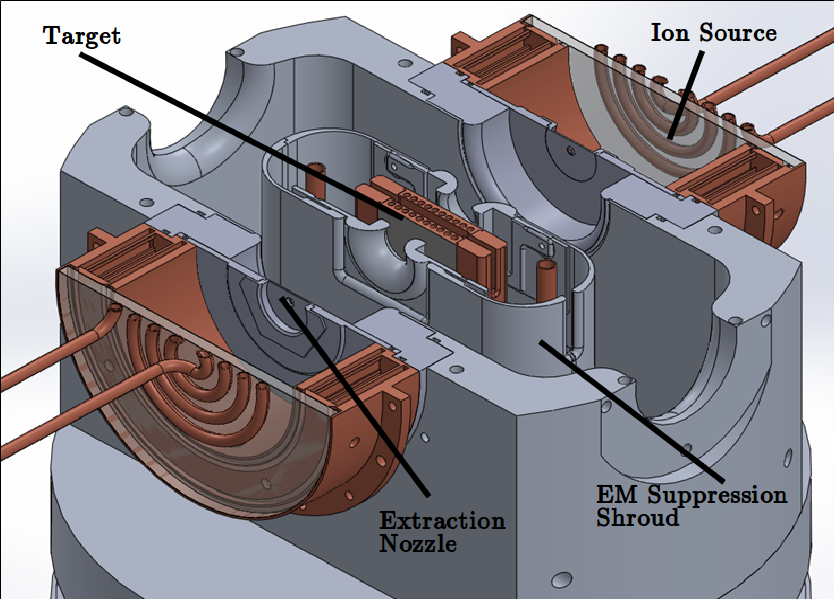
\includegraphics[width=\textwidth]{./figures/target2.png}
        \subfigimg[width=\linewidth]{}{./figures/87gY.pdf}{50}
%         \caption{Decay curve for the $\beta^-$ decay of \ce{^{116}In}.}
                 \refstepcounter{subfigure}\label{fig:87gY}
    \end{subfigure}
%     \caption{Decay curves used to verify photopeak transition assignment. (a) Decay curve for the isomeric transition of \ce{^{115m}In}, (b) decay curve for the isomeric transition of \ce{^{113m}In}, (c) decay curve for the $\beta^-$ decay of \ce{^{116}In}, and (d) decay curve for the $\beta^+$ decay of \ce{^{64}Cu}.}
     \label{fig:xs_curves_p4}
\end{figure*}

\begin{figure*}
    \centering
%      \begin{subfigure}[t]{0.495\textwidth}
%         \centering
% %         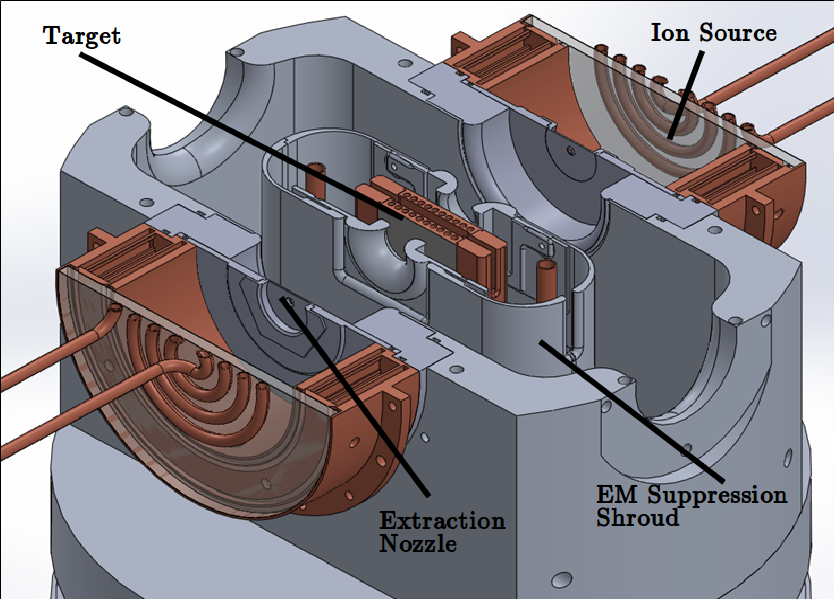
\includegraphics[width=\textwidth]{./figures/target2.png}
%         \subfigimg[width=\linewidth]{}{./figures/87gY.pdf}{50}
% %         \caption{Decay curve for the $\beta^-$ decay of \ce{^{116}In}.}
%                  \refstepcounter{subfigure}\label{fig:87gY}
%     \end{subfigure}
    \begin{subfigure}[t]{0.495\textwidth}
        \centering
%         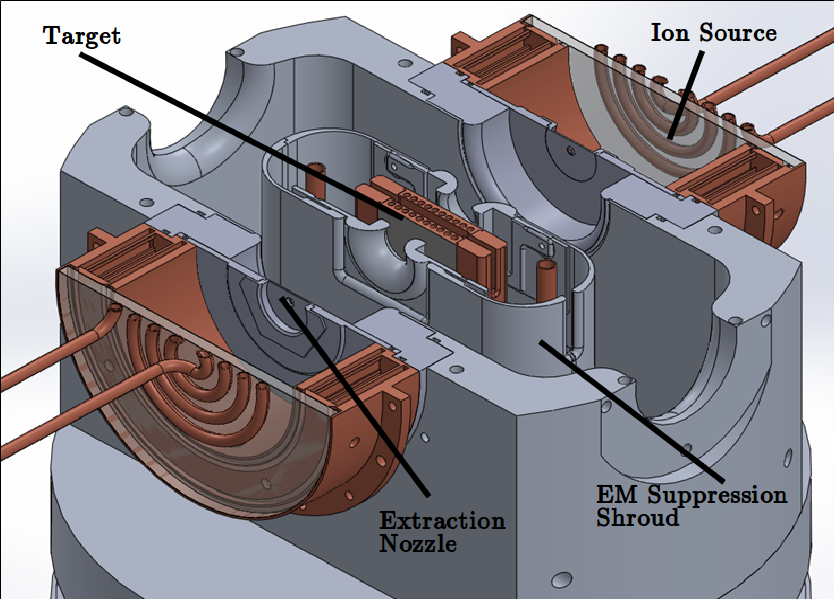
\includegraphics[width=\textwidth]{./figures/target2.png}
        \subfigimg[width=\linewidth]{}{./figures/87mY.pdf}{50}
%         \caption{Decay curve for the $\beta^-$ decay of \ce{^{116}In}.}
                 \refstepcounter{subfigure}\label{fig:87mY}
    \end{subfigure}
    \begin{subfigure}[t]{0.495\textwidth}
        \centering
%         \includegraphics[width=\columnwidth]{./figures/Capture.PNG}
        \subfigimg[width=\linewidth]{}{./figures/87Zr.pdf}{50}
%         \caption{ Decay curve for the $\beta^+$ decay of \ce{^{64}Cu}.}
        \refstepcounter{subfigure} \label{fig:87Zr}
    \end{subfigure}%
    \\
    \begin{subfigure}[t]{0.495\textwidth}
        \centering
%         \includegraphics[width=\columnwidth]{./figures/Capture.PNG}
        \subfigimg[width=\linewidth]{}{./figures/88Y.pdf}{50}
%         \caption{ Decay curve for the isomeric transition of \ce{^{115m}In}.}
         \refstepcounter{subfigure}\label{fig:88Y}
    \end{subfigure}%
     \begin{subfigure}[t]{0.495\textwidth}
        \centering
%         \includegraphics[width=\columnwidth]{./figures/Capture.PNG}
%         \includegraphics[scale=0.6]{./figures/391keV_curve2.png}
        \subfigimg[width=\linewidth]{}{./figures/88Zr.pdf}{50}
%         \caption{ Decay curve for the isomeric transition of \ce{^{113m}In}.}
         \refstepcounter{subfigure}\label{fig:88Zr}
    \end{subfigure}%
    \\
         \begin{subfigure}[t]{0.495\textwidth}
        \centering
%         \includegraphics[width=\columnwidth]{./figures/Capture.PNG}
%         \includegraphics[scale=0.6]{./figures/391keV_curve2.png}
        \subfigimg[width=\linewidth]{}{./figures/89Nb.pdf}{50}
%         \caption{ Decay curve for the isomeric transition of \ce{^{113m}In}.}
         \refstepcounter{subfigure}\label{fig:89Nb}
    \end{subfigure}%
    \begin{subfigure}[t]{0.495\textwidth}
        \centering
%         \includegraphics[width=\columnwidth]{./figures/Capture.PNG}
%         \includegraphics[scale=0.6]{./figures/391keV_curve2.png}
        \subfigimg[width=\linewidth]{}{./figures/89gNb.pdf}{50}
%         \caption{ Decay curve for the isomeric transition of \ce{^{113m}In}.}
         \refstepcounter{subfigure}\label{fig:89gNb}
    \end{subfigure}%
%     \caption{Decay curves used to verify photopeak transition assignment. (a) Decay curve for the isomeric transition of \ce{^{115m}In}, (b) decay curve for the isomeric transition of \ce{^{113m}In}, (c) decay curve for the $\beta^-$ decay of \ce{^{116}In}, and (d) decay curve for the $\beta^+$ decay of \ce{^{64}Cu}.}
     \label{fig:xs_curves_p8}
\end{figure*}

\begin{figure*}
    \centering    
%          \begin{subfigure}[t]{0.495\textwidth}
%         \centering
% %         \includegraphics[width=\columnwidth]{./figures/Capture.PNG}
% %         \includegraphics[scale=0.6]{./figures/391keV_curve2.png}
%         \subfigimg[width=\linewidth]{}{./figures/89gNb.pdf}{50}
% %         \caption{ Decay curve for the isomeric transition of \ce{^{113m}In}.}
%          \refstepcounter{subfigure}\label{fig:89gNb}
%     \end{subfigure}%
    \begin{subfigure}[t]{0.495\textwidth}
        \centering
%         \includegraphics[width=\textwidth]{./figures/target2.png}
        \subfigimg[width=\linewidth]{}{./figures/89mNb.pdf}{50}
%         \caption{Decay curve for the $\beta^-$ decay of \ce{^{116}In}.}
                 \refstepcounter{subfigure}\label{fig:89mNb}
    \end{subfigure}
     \begin{subfigure}[t]{0.495\textwidth}
        \centering
%         \includegraphics[width=\columnwidth]{./figures/Capture.PNG}
        \subfigimg[width=\linewidth]{}{./figures/89Zr.pdf}{50}
%         \caption{ Decay curve for the $\beta^+$ decay of \ce{^{64}Cu}.}
        \refstepcounter{subfigure} \label{fig:89Zr}
    \end{subfigure}%
    \\
    \begin{subfigure}[t]{0.495\textwidth}
        \centering
%         \includegraphics[width=\textwidth]{./figures/target2.png}
        \subfigimg[width=\linewidth]{}{./figures/91mNb.pdf}{50}
%         \caption{Decay curve for the $\beta^-$ decay of \ce{^{116}In}.}
                 \refstepcounter{subfigure}\label{fig:91mNb}
    \end{subfigure}
     \begin{subfigure}[t]{0.495\textwidth}
        \centering
%         \includegraphics[width=\columnwidth]{./figures/Capture.PNG}
        \subfigimg[width=\linewidth]{}{./figures/92mNb.pdf}{50}
%         \caption{ Decay curve for the $\beta^+$ decay of \ce{^{64}Cu}.}
        \refstepcounter{subfigure} \label{fig:92mNb}
    \end{subfigure}%
    \\
    \begin{subfigure}[t]{0.495\textwidth}
        \centering
%         \includegraphics[width=\columnwidth]{./figures/Capture.PNG}
        \subfigimg[width=\linewidth]{}{./figures/93mMo.pdf}{50}
%         \caption{ Decay curve for the isomeric transition of \ce{^{115m}In}.}
         \refstepcounter{subfigure}\label{fig:93mMo}
    \end{subfigure}%
%     \caption{Decay curves used to verify photopeak transition assignment. (a) Decay curve for the isomeric transition of \ce{^{115m}In}, (b) decay curve for the isomeric transition of \ce{^{113m}In}, (c) decay curve for the $\beta^-$ decay of \ce{^{116}In}, and (d) decay curve for the $\beta^+$ decay of \ce{^{64}Cu}.}
     \label{fig:xs_curves_p7}
\end{figure*}

% \begin{figure*}
%     \centering
%     \begin{subfigure}[t]{0.495\textwidth}
%         \centering
% %         \includegraphics[width=\columnwidth]{./figures/Capture.PNG}
%         \subfigimg[width=\linewidth]{}{./figures/93mMo.pdf}{50}
% %         \caption{ Decay curve for the isomeric transition of \ce{^{115m}In}.}
%          \refstepcounter{subfigure}\label{fig:93mMo}
%     \end{subfigure}%
% %      \begin{subfigure}[t]{0.495\textwidth}
% %         \centering
% % %         \includegraphics[width=\columnwidth]{./figures/Capture.PNG}
% % %         \includegraphics[scale=0.6]{./figures/391keV_curve2.png}
% %         \subfigimg[width=\linewidth]{}{./figures/91mNb.pdf}{50}
% % %         \caption{ Decay curve for the isomeric transition of \ce{^{113m}In}.}
% %          \refstepcounter{subfigure}\label{fig:91mNb}
% %     \end{subfigure}%
% %     \\
% %     \begin{subfigure}[t]{0.495\textwidth}
% %         \centering
% % %         \includegraphics[width=\textwidth]{./figures/target2.png}
% %         \subfigimg[width=\linewidth]{}{./figures/92mNb.pdf}{50}
% % %         \caption{Decay curve for the $\beta^-$ decay of \ce{^{116}In}.}
% %                  \refstepcounter{subfigure}\label{fig:92mNb}
% %     \end{subfigure}
% %      \begin{subfigure}[t]{0.495\textwidth}
% %         \centering
% % %         \includegraphics[width=\columnwidth]{./figures/Capture.PNG}
% %         \subfigimg[width=\linewidth]{}{./figures/93mMo.pdf}{50}
% % %         \caption{ Decay curve for the $\beta^+$ decay of \ce{^{64}Cu}.}
% %         \refstepcounter{subfigure} \label{fig:93mMo}
% %     \end{subfigure}%
% %     \caption{Decay curves used to verify photopeak transition assignment. (a) Decay curve for the isomeric transition of \ce{^{115m}In}, (b) decay curve for the isomeric transition of \ce{^{113m}In}, (c) decay curve for the $\beta^-$ decay of \ce{^{116}In}, and (d) decay curve for the $\beta^+$ decay of \ce{^{64}Cu}.}
%      \label{fig:xs_curves_p5}
% \end{figure*}




% 
% 
\section{Measured isomer-to-ground state branching ratios } \label{ibr_figures}

Plots of the isomer-to-ground state ratios measured in this work are presented here, in comparison with literature data and reaction modeling codes \cite{MICHEL1997153,Ditroi2008,Titarenko2011,Graves2016}.





\begin{figure*}
    \centering
    \begin{subfigure}[t]{0.495\textwidth}
        \centering
%         \includegraphics[width=\columnwidth]{./figures/Capture.PNG}
        \subfigimg[width=\linewidth]{}{./figures/52Mn_IBR.pdf}{50}
%         \caption{ Decay curve for the isomeric transition of \ce{^{115m}In}.}
         \refstepcounter{subfigure}\label{fig:52Mn_IBR}
    \end{subfigure}%
     \begin{subfigure}[t]{0.495\textwidth}
        \centering
%         \includegraphics[width=\columnwidth]{./figures/Capture.PNG}
%         \includegraphics[scale=0.6]{./figures/391keV_curve2.png}
        \subfigimg[width=\linewidth]{}{./figures/58Co_IBR.pdf}{50}
%         \caption{ Decay curve for the isomeric transition of \ce{^{113m}In}.}
         \refstepcounter{subfigure}\label{fig:58Co_IBR}
    \end{subfigure}%
    \\
    \begin{subfigure}[t]{0.495\textwidth}
        \centering
%         \includegraphics[width=\textwidth]{./figures/target2.png}
        \subfigimg[width=\linewidth]{}{./figures/85Y_IBR.pdf}{50}
%         \caption{Decay curve for the $\beta^-$ decay of \ce{^{116}In}.}
                 \refstepcounter{subfigure}\label{fig:85Y_IBR}
    \end{subfigure}
     \begin{subfigure}[t]{0.495\textwidth}
        \centering
%         \includegraphics[width=\columnwidth]{./figures/Capture.PNG}
        \subfigimg[width=\linewidth]{}{./figures/87Y_IBR.pdf}{50}
%         \caption{ Decay curve for the $\beta^+$ decay of \ce{^{64}Cu}.}
        \refstepcounter{subfigure} \label{fig:87Y_IBR}
    \end{subfigure}%
    \\
    \begin{subfigure}[t]{0.495\textwidth}
        \centering
%         \includegraphics[width=\textwidth]{./figures/target2.png}
        \subfigimg[width=\linewidth]{}{./figures/89Nb_IBR.pdf}{50}
%         \caption{Decay curve for the $\beta^-$ decay of \ce{^{116}In}.}
                 \refstepcounter{subfigure}\label{fig:89Nb_IBR}
    \end{subfigure}
     \label{fig:ibr_curves}
\end{figure*}


% 
% 
% % \begin{figure}[h]
% %  \centering
% %  \includegraphics[scale=0.7]{./hw04/fit110Ru240-cropped.pdf}
% %  % fit110Ru240.ps: 570x750 pixel, 72dpi, 20.11x26.46 cm, bb=0 0 570 750
% %  \caption{Fit to the \ce{^{110}Ru} 240.7 keV peak and its surroundings.}
% %  \label{fig:110Ru240}
% % \end{figure}
% % 

% \twocolumn

%% References with BibTeX database:

% \bibliographystyle{elsarticle-num}
% \bibliographystyle{elsarticle-harv}
% \bibliographystyle{elsarticle-num-names}
% \bibliography{<your-bib-database>}
% \addcontentsline{toc}{chapter}{Bibliography}
\bibliographystyle{elsarticle-num}
% \bibliographystyle{apsrev4-1}
% \bibliographystyle{ieeetr}
\bibliography{../../library}
% \thispagestyle{fancyTOC}




%% Authors are advised to use a BibTeX database file for their reference list.
%% The provided style file elsarticle-num.bst formats references in the required Procedia style

%% For references without a BibTeX database:

% \begin{thebibliography}{00}

%% \bibitem must have the following form:
%%   \bibitem{key}...
%% 

% \bibitem{}

% \end{thebibliography}

\end{document}

%%
%% End of file `ecrc-template.tex'. 